%%%%%%%%%%%%%%%%%%%%%%%%%%%%%%%%%%%%%%%%%%%%%%%%%%%%%%%%%%%%%%%%%%%%%%%%%%%
%%
%% Filename: 	spec.tex
%%
%% Project:	ZipCPU -- a small, lightweight, RISC CPU soft core
%%
%% Purpose:	This LaTeX file contains all of the documentation/description
%%		currently provided with this ZipCPU soft core.  It supersedes
%%		any information about the instruction set or CPUs found
%%		elsewhere.  It's not nearly as interesting, though, as the PDF
%%		file it creates, so I'd recommend reading that before diving
%%		into this file.  You should be able to find the PDF file in
%%		the SVN distribution together with this PDF file and a copy of
%%		the GPL-3.0 license this file is distributed under.  If not,
%%		just type 'make' in the doc directory and it (should) build
%%		without a problem.
%%		
%%
%% Creator:	Dan Gisselquist
%%		Gisselquist Technology, LLC
%%
%%%%%%%%%%%%%%%%%%%%%%%%%%%%%%%%%%%%%%%%%%%%%%%%%%%%%%%%%%%%%%%%%%%%%%%%%%%
%%
%% Copyright (C) 2015, Gisselquist Technology, LLC
%%
%% This program is free software (firmware): you can redistribute it and/or
%% modify it under the terms of  the GNU General Public License as published
%% by the Free Software Foundation, either version 3 of the License, or (at
%% your option) any later version.
%%
%% This program is distributed in the hope that it will be useful, but WITHOUT
%% ANY WARRANTY; without even the implied warranty of MERCHANTIBILITY or
%% FITNESS FOR A PARTICULAR PURPOSE.  See the GNU General Public License
%% for more details.
%%
%% You should have received a copy of the GNU General Public License along
%% with this program.  (It's in the $(ROOT)/doc directory, run make with no
%% target there if the PDF file isn't present.)  If not, see
%% <http://www.gnu.org/licenses/> for a copy.
%%
%% License:	GPL, v3, as defined and found on www.gnu.org,
%%		http://www.gnu.org/licenses/gpl.html
%%
%%
%%%%%%%%%%%%%%%%%%%%%%%%%%%%%%%%%%%%%%%%%%%%%%%%%%%%%%%%%%%%%%%%%%%%%%%%%%%
%
%
%
% From TI about DSPs vs FPGAs:
%	www.ti.com/general/docs/video/foldersGallery.tsp?bkg=gray
%	&gpn=35145&familyid=1622&keyMatch=DSP Breaktime Episode Three
%	&tisearch=Search-EN-Everything&DCMP=leadership
%	&HQS=ep-pro-dsp-leadership-problog-150518-v-en
%
%	FPGA's are annoyingly faster, cheaper, and not quite as power hungry
%	as they used to be.
%
%	Why would you choose DSPs over FPGAs?  If you care about size,
%	if you care about power, or happen to have a complicated algorithm
%	that just isn't simply doing the same thing over and over
%
%	For complex algorithms that change over time.  Each have their strengths
%	sometimes you can use both.
%
%	"No assembly required" -- TI tools all C programming, very GUI based
%	environment, very little optimization by hand ...
%
%
% The FPGA's Achille's heel: Reconfigurability.  It is very difficult, although
% I'm sure major vendors will tell you not impossible, to reconfigure an FPGA
% based upon the need to process time-sensitive data.  If you need one of two
% algorithms, both which will fit on the FPGA individually but not together,
% switching between them on the fly is next to impossible, whereas switching
% algorithm within a CPU is not difficult at all.  For example, imagine 
% receiving a packet and needing to apply one of two data algorithms on the
% packet before sending it back out, and needing to do so fast.  If both
% algorithms don't fit in memory, where does the packet go when you need to
% swap one algorithm out for the other?  And what is the cost of that "context"
% swap?
%
%
\documentclass{gqtekspec}
\usepackage{import}
\usepackage{bytefield}	% Install via apt-get install texlive-science
% \graphicspath{{../gfx}}
\project{ZipCPU}
\title{Specification}
\author{Dan Gisselquist, Ph.D.}
\email{dgisselq (at) ieee.org}
\revision{Rev.~1.1}
\definecolor{webred}{rgb}{0.5,0,0}
\definecolor{webgreen}{rgb}{0,0.4,0}
\hypersetup{
	ps2pdf,
	pdfpagelabels,
	hypertexnames,
	pdfauthor={Dan Gisselquist},
	pdfsubject={ZipCPU},
	anchorcolor= black,
	colorlinks = true,
	linkcolor  = webred,
	citecolor  = webgreen
}
\begin{document}
\pagestyle{gqtekspecplain}
\titlepage
\begin{license}
Copyright (C) \theyear\today, Gisselquist Technology, LLC

This project is free software (firmware): you can redistribute it and/or
modify it under the terms of  the GNU General Public License as published
by the Free Software Foundation, either version 3 of the License, or (at
your option) any later version.

This program is distributed in the hope that it will be useful, but WITHOUT
ANY WARRANTY; without even the implied warranty of MERCHANTIBILITY or
FITNESS FOR A PARTICULAR PURPOSE.  See the GNU General Public License
for more details.

You should have received a copy of the GNU General Public License along
with this program.  If not, see \hbox{$<$http://www.gnu.org/licenses/$>$} for
a copy.
\end{license}
\begin{revisionhistory}
2.0 & 1/18/2017 & Gisselquist & Switched from 32--bit to 8--bit bytes.\\\hline
1.1 & 11/28/2016 & Gisselquist & Moved the ZipSystem address to {\tt 0xff000000} base.\\\hline
1.0 & 11/4/2016 & Gisselquist & Major rewrite,
			includes compiler info\\\hline
0.91& 7/16/2016 & Gisselquist & Described three more CC bits\\\hline
0.9 & 4/20/2016 & Gisselquist & Modified ISA: LDIHI replaced with MPY,
	MPYU and MPYS replaced with MPYUHI, and MPYSHI respectively.  LOCK
	instruction now permits an intermediate ALU operation. \\\hline
0.8 & 1/28/2016 & Gisselquist & Reduced complexity early branching \\\hline
0.7 & 12/22/2015 & Gisselquist & New Instruction Set Architecture \\\hline
0.6 & 11/17/2015 & Gisselquist & Added graphics to illustrate pipeline discussion.\\\hline
0.5 & 9/29/2015 & Gisselquist & Added pipelined memory access discussion.\\\hline
0.4 & 9/19/2015 & Gisselquist & Added DMA controller, improved stall information, and self--assessment info.\\\hline
0.3 & 8/22/2015 & Gisselquist & First completed draft\\\hline
0.2 & 8/19/2015 & Gisselquist & Still Draft, more complete \\\hline
0.1 & 8/17/2015 & Gisselquist & Incomplete First Draft \\\hline
\end{revisionhistory}
% Revision History
% Table of Contents, named Contents
\tableofcontents
\listoffigures
\listoftables
\begin{preface}
Many people have asked me why I am building the ZipCPU. ARM processors are
good and effective.  Xilinx makes and markets Microblaze, Altera Nios, and both
have better toolsets than the ZipCPU will ever have. OpenRISC is also
available, RISC--V may be replacing it. Why build a new processor?

The easiest, most obvious answer is the simple one: Because I can.

There's more to it though. There's a lot of things that I would like to do with
a processor, and I want to be able to do them in a vendor independent fashion.
First, I would like to be able to place this processor inside an FPGA.  Without
paying royalties, ARM is out of the question.  I would then like to be able to
generate Verilog code, both for the processor and the system it sits within,
that can run equivalently on both Xilinx, Altera, and Lattice chips, and that
can be easily ported from one manufacturer's chipsets to another. Even more,
before purchasing a chip or a board, I would like to know that my soft core
works. I would like to build a test bench to test components with, and
Verilator is my chosen test bench. This forces me to use all Verilog, and it
prevents me from using any proprietary cores. For this reason, Microblaze and
Nios are out of the question.

Why not OpenRISC? Because the ZipCPU has different goals.  OpenRISC is designed
to be a full featured CPU.  The ZipCPU was designed to be a simple, resource
friendly, CPU.  The result is that it is easy to get a ZipCPU program running
on bare hardware for a special purpose application--such as what FPGAs were
designed for, but getting a full featured
Linux distribution running on the ZipCPU may just be beyond my grasp.  Further,
the OpenRISC ISA is very complex, defining over 200~instructions--even though
it has never been fully implemented.  The ZipCPU on the other hand has only
a small handful of instructions, and all but the Floating Point instructions
have already been fully implemented.

My final reason is that I'm building the ZipCPU as a learning experience. The
ZipCPU has allowed me to learn a lot about how CPUs work on a very micro
level. For the first time, I am beginning to understand many of the Computer
Architecture lessons from years ago.

To summarize: Because I can, because it is open source, because it is light
weight, and as an exercise in learning. 

\end{preface}

\chapter{Introduction}
\pagenumbering{arabic}
\setcounter{page}{1}

The goal of the ZipCPU was to be a very simple CPU.   You might think of it as
a poor man's alternative to the OpenRISC architecture.  You might also think of
it as an Open Source microcontroller.
For this reason, all instructions have been designed to be as simple as
possible, and the base instructions are all designed to be executed in one
instruction cycle per instruction, barring pipeline stalls.\footnote{The
exceptions to this rule are the multiply, divide, and load/store instructions.
Once the floating point unit is built, I anticipate these will also be
exceptions to this rule.}  Indeed, even the bus has been simplified to a
constant 32-bit width, with no option for more or less.  This has resulted in
the choice to drop push and pop instructions, pre-increment and post-decrement
addressing modes, the integrated memory management unit (MMU), and
more.\footnote{A not--so integrated MMU is currently under development.}

For those who like buzz words, the ZipCPU is:
\begin{itemize}
\item A 32-bit CPU: All registers are 32-bits, addresses are 32-bits,
		instructions are 32-bits wide, etc.
\item A RISC CPU.  There is no microcode for executing instructions.  All
	instructions are designed to be completed in one clock cycle.
\item A Load/Store architecture.  (Only load and store instructions
		can access memory.)
\item Wishbone compliant.  All peripherals are accessed just like
		memory across this bus.
\item A Von-Neumann architecture.  The instructions and data share a 
		common bus.
\item A pipelined architecture, having stages for {\bf Prefetch},
	{\bf Decode}, {\bf Read-Operand}, a combined stage containing
	the {\bf ALU}, {\bf Memory}, {\bf Divide}, and {\bf Floating Point}
	units, and then the final {\bf Write-back} stage. 
		See Fig.~\ref{fig:cpu}
\begin{figure}\begin{center}
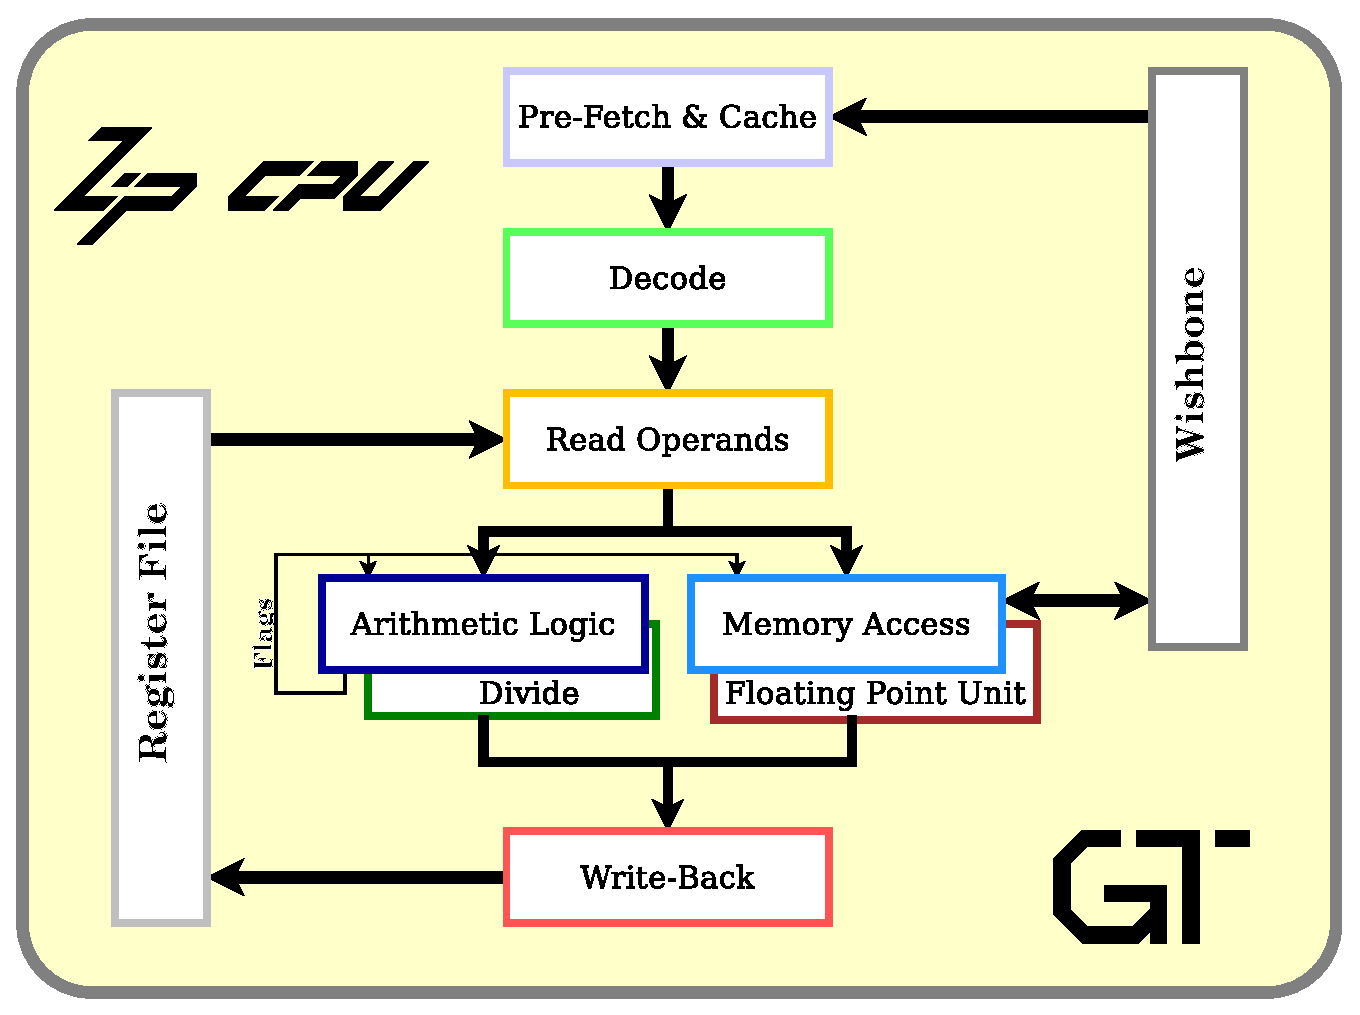
\includegraphics[width=3.5in]{../gfx/cpu.eps}
\caption{ZipCPU internal pipeline architecture}\label{fig:cpu}
\end{center}\end{figure}
		for a diagram of this structure.
\item Completely open source, licensed under the GPL.\footnote{Should you
	need a copy of the ZipCPU licensed under other terms, please 
	contact me.}
\end{itemize}

The ZipCPU also has one very unique feature: the ability to do pipelined loads
and stores.  This allows the CPU to access on-chip memory at one access per
clock, minus any stalls for the initial access.

\section{Characteristics of a SwiC}

This section might also be called {\em the ZipCPU philosophy}.  It discusses
the basis for the ZipCPU design decisions, and why a low logic count CPU
is or can be a good thing.

Many other FPGA processors have been defined to be good Systems on a Chip, or 
SoC's.  The entire goal of such designs, then, is to provide an interface
to the processor and its external environment.  This is not the case with the
ZipCPU.  Instead, we shall define a new concept, that of a soft core internal to
an FPGA, as a ``System within a Chip,'' or a SwiC.  SwiCs have some very
unique properties internal to them that have influenced the design of the
ZipCPU.  Among these are the bus, memory, and available peripherals.

Many other approaches to soft core CPU's employ a Harvard architecture. 
This allows these other CPU's to have two separate bus structures: one for the
program fetch, and the other for the memory.  Indeed, Xilinx's proprietary
Microblaze processor
goes so far as to support four busses: two for cacheable memory, and two for
peripherals, with each of those split between instructions and data.  The
ZipCPU on the other hand is fairly unique in its approach because it uses a
Von Neumann architecture, requiring only one bus within any FPGA.  This
structure was chosen for its simplicity.  Having only the one bus helps to
minimize real-estate, logic, and the number of wires that need to be passed
back and forth, while maintaining a high clock speed.  The disadvantage is
that both prefetch and memory access units need to contend for time on the 
same bus.

Soft core's within an FPGA have an additional characteristic regarding
memory access: it is slow.  While memory on chip may be accessed at a single
cycle per access, small FPGA's often have only a limited amount of memory on
chip.  Going off chip, however, is expensive.  Two examples will prove this
point.  On
the XuLA2 board, Flash can be accessed at 128~cycles per 32--bit word,
or 64~cycles per subsequent word in a pipelined architecture.  Likewise, the
SDRAM chip on the XuLA2 board allows a 6~cycle access for a write, 10~cycles
per read, and 2~cycles for any subsequent pipelined access read or write.
Either way you look at it, this memory access will be slow and this doesn't
account for any logic delays should the bus implementation logic get
complicated.

As may be noticed from the above discussion about memory speed, a second
characteristic of memory is sequential memory accesses may be optimized for
minimal delays (pipelined), and that pipelined memory access is faster than
non--pipelined access.  Therefore, a SwiC soft core should support pipelined
operations, but it should also allow a higher priority subsystem to get access
to the bus (no starvation).

As a further characteristic of SwiC memory options, on-chip cache's are
expensive.  If you want to have a minimum of logic, cache logic may not be
the highest on the priority list.  Any SwiC capable processor must be able
to either be built without caches, or to scale up or down the logic required
by any cache.

In sum, memory is slow.  While one processor on one FPGA may be able to fill
its pipeline, the same processor on another FPGA may struggle to get more than
one instruction at a time into the pipeline.  Any SwiC must be able to deal
with both cases: fast and slow memories.

A final characteristic of SwiC's within FPGA's is the peripherals. 
Specifically, FPGA's are highly reconfigurable.  Soft peripherals can easily
be created on chip to support the SwiC if necessary.  As an example, a simple
30-bit peripheral could easily support reversing 30-bit numbers: a read from
the peripheral returns its bit--reversed address.  This is cheap within an
FPGA, but expensive in instructions.  Reading from another 16--bit peripheral
might calculate a sine function, where the 16--bit address internal to the
peripheral was the angle of the sine wave.

Indeed, anything that must be done fast within an FPGA is likely to already
be done--elsewhere in the fabric.  Further, the application designer gets to
choose what tasks are so important they need fabric dedicated to them, and which
ones can be done more slowly in a CPU.  This leaves the CPU with the simple role
of solely handling sequential tasks, and tasks that need a lot of state.

This means that the SwiC needs to live within a very unique environment,
separate and different from the traditional SoC.  That isn't to say that a 
SwiC cannot be turned into a SoC, just that this SwiC has not been designed
for that purpose.  Indeed, some of the best examples of the ZipCPU are
System on a Chip examples.

\section{Scope}\label{sec:limits}

The ZipCPU is itself nothing more than a CPU that can be placed within a 
larger design.  It is not a System on a Chip, but it can be used to create
a system on a chip.  As a result, this document will not discuss more than a
small handful of CPU--related peripherals, as the actual peripherals used
within a design will vary from one design to the next.  Further, because
control access will vary from one environment to the next, this document will
not discuss any host control programs, leaving those to be discussed and defined
together with the environments the ZipCPU is placed within.

\chapter{CPU Architecture}\label{chap:arch}

This chapter describes the general architecture of the ZipCPU.  It first
discusses
the configuration options to the CPU and then breaks into two threads. These
last two threads are a discussion of the internals of the ZipCPU, such as its 
instruction set architecture and the details and consequences of it, and then
the external architecture describing how the ZipCPU fits into the systems
surrounding it, and what those systems must do to support it.  Specifically,
the external architecture section will discuss both the ZipSystem, the
peripherals provided by it, as well as the debug interface.

\section{Build Options/defines}\label{ssec:build-options}

One problem with a simple goal such as being light on logic, is that some
architectures have some needs, others have other needs.  What is light logic
in some architectures might consume all the available logic in others.
As an example, the CMod~S6 board built by Digilent uses a very spare Xilinx
Spartan~6 LX4 FPGA.  This FPGA doesn't have enough look up tables (LUTs) to
support pipelined mode, whereas another project running on a XuLA2 LX25 board
made by Xess, having a Spartan~6 LX25 on board, has more than enough logic
to support a pipelined mode.   Very quickly it becomes clear that LUTs can be
traded for performance.

To make this possible, the ZipCPU has both a configuration file as well as a
set of parameters that it can be built with.  Often, those parameters can
override the configuration file, but not all configuration file changes can
be overridden.  Several options are available within the configuration file,
such as making the Zip CPU pipelined or not, able to handle a faster clock
with more stalls or a slower clock with no stalls, etc.

The {\tt cpudefs.v} file encapsulates those control options.  It contains a 
series of {\tt `define} statements that can either be commented or left
active.  If active, the option is considered to be in effect.  The number of
LUTs the Zip CPU uses varies dramatically with the options defined in this file.
This section will outline the various configuration options captured by this
file.

The first couple of options control the Zip CPU instruction set, and how
it handles various instructions within the set:


{\tt OPT\_MULTIPLY} controls whether or not the multiply is built and included
in the ALU by default, and if it is which of several multiply options is 
selected.  Unlike many of the defines that follow within {\tt cpudefs.v} that
are either defined or not, this option requires a value.  A value of zero means
no multiply support, whereas a value of one, two, or three, means that a
multiply will be included that takes one, two, or three clock cycles to
complete.  The option, however, only controls the default value that the
{\tt IMPLEMENT\_MPY} parameter to the CPU, having the same interpretation, is
given.  Because this is just the default value, it can easily be overridden
upon instantiation.  If the {\tt IMPLEMENT\_MPY} parameter is set to zero,
then any attempt to execute a multiply instruction will cause an illegal
instruction exception.

{\tt OPT\_DIVIDE} controls whether or not the divide instruction is built and
included into the ZipCPU by default.  Set this option and the
{\tt IMPLEMENT\_DIVIDE} parameter will have a default value of one, meaning that
unless it is overridden with zero, the divide unit will be included.    If the
divide is not included, then any attempt to use a divide instruction will
create an illegal instruction exception that will send the CPU into supervisor
mode.

{\tt OPT\_IMPLEMENT\_FPU} will (one day) control whether or not the floating
point unit (once I have one) is built and included into the ZipCPU by default.
This option sets the {\tt IMPLEMENT\_FPU} parameter to one, so alternatively
it can be set and adjusted upon instantiation.  If the floating point unit is
not included then, as with the multiply and divide, any floating point
instruction will result in an illegal instruction exception that will send the
CPU into supervisor mode.

{\tt OPT\_SINGLE\_FETCH} controls whether or not the prefetch has a cache, and 
whether or not it can issue one instruction per clock.  When set, the
prefetch has no cache, and only one instruction is fetched at any given time.
This effectively sets the CPU so that only one instruction is ever 
in the pipeline at a time, and hence you may think of this as a ``no 
pipeline'' option.  However, since the pipeline uses so much area on the FPGA,
this is an important option to use in trimming down used logic if necessary. 
Hence, it needs to be maintained for that purpose.  Be aware, though, setting
this option will disable all pipelining, and therefore will drop your
performance by a factor of 8x or even more.

I recommend only defining or enabling this option if you {\em need} to,
such as if area is tight and speed isn't as important.  Otherwise, leave the
option undefined since the pipelined options have a much better speed
performance.

The next several options are pipeline optimization options.  They make no
sense in a single instruction fetch mode, hence they are all disabled if
{\tt OPT\_SINGLE\_FETCH} is defined.

{\tt OPT\_PIPELINED} is the natural result and opposite of using the single 
instruction fetch unit.  It is an internal parameter that doesn't need user
adjustment, but if you look through the {\tt cpudefs.v} file you may see
and notice it.  If you have not set the {\tt OPT\_SINGLE\_FETCH} parameter,
{\tt cpudefs.v} will set the {\tt OPT\_PIPELINED} option.  This is more for
readability than anything else, since {\tt OPT\_PIPELINED} makes more
intuitive readability sense than {\tt OPT\_SINGLE\_FETCH}.  In other words,
define or comment out {\tt OPT\_SINGLE\_FETCH}, and let {\tt OPT\_PIPELINED} be
taken care of automatically.

Assuming you have chosen not to define {\tt OPT\_SINGLE\_FETCH},
{\tt OPT\_TRADITIONAL\_PFCACHE} allows you to switch between one of two
prefetch cache modules.  If enabled (recommended), a more traditional cache 
will be implemented in the CPU.  This more traditional cache reduces
the stall count tremendously over the alternative pipeline cache, and its
LUT usage is quite competitive.  As there is little downside to defining
this option if pipelining is enabled, I would recommend including it.

The alternative prefetch and cache, sometimes called the pipeline cache, tries
to read instructions ahead of where they are needed, while maintaining what it
has read in a cache.  That cache is cleared anytime you jump outside of its
window, and it often competes with the CPU for access to the bus.  These
two characteristics make this alternative bus often less than optimal.


{\tt OPT\_EARLY\_BRANCHING} is an attempt to execute a {\tt BRA} (branch or
jump) statement as early
in the pipeline as possible, to avoid as many pipeline stalls on a branch as
possible.  As an example, if you have {\tt OPT\_TRADITIONAL\_PFCACHE} defined
as well, then branches within the cache will only cost a single stall cycle.
Indeed, using early branching, a {\tt BRA} instruction can be used as the
compiler's branch prediction optimizer: {\tt BRA}'s barely stall, while
branches on conditions will always suffer about 6~stall cycles.  Setting
this option causes the parameter, {\tt EARLY\_BRANCHING}, to be set to one,
so it can be overridden upon instantiation.

Given the performance benefits achieved by early branching, setting this flag
is highly recommended.

{\tt OPT\_PIPELINED\_BUS\_ACCESS} controls whether or not memory
instructions can take advantage of the pipelined wishbone bus.  To be
eligible, the operations to be pipelined must be adjacent, must be all
loads or all stores, and the addresses must all use the same base
address register and either have identical immediate offsets, or immediate
offsets that increase by one for each instruction.  Further, the
string of load (or store) instructions must all have the same conditional
(if any).  Currently, this approach and benefit is most effectively used
when saving registers to or restoring registers from the stack at the
beginning/end of a procedure, when using assembly optimized programs, or
when doing a context swap.

I recommend setting this flag, for performance reasons, especially if your
wishbone bus implementation can handle pipelined bus accesses.  The logic
impact of this setting is minimal, the performance impact can be significant.

{\tt OPT\_CIS} includes within the instruction set the Very Long Instruction
Word packing, which packs up to two instructions within each instruction word.
Non--packed instructions will still execute as normal, this just enables the
decoding and running of packed instructions.

The two next options, {\tt INCLUDE\_DMA\_CONTROLLER} and
{\tt INCLUDE\_ACCOUNTING\_COUNTERS}
control whether the DMA controller is included in the ZipSystem, and
whether or not the eight accounting timers are also included.  Set these to
include the respective peripherals, comment them out not to.  These only 
affect the ZipSystem implementation, and not any ZipBones implementations.

Finally, if you find yourself needing to debug the core and specifically
needing to get a trace from the core to find out why something specifically
failed, you may find it useful to define {\tt DEBUG\_SCOPE}.  This will add a
32--bit debug output from the core, as the last argument to the core, to the
ZipSystem, or even to ZipBones.  The actual definition and composition of
this debugging bit--field changes from one implementation to the next,
depending upon needs and necessities, so please look at the code at the
bottom of {\tt zipcpu.v} for more details.

That ends our discussion of CPU options, but there remain several
implementation parameters that can be defined with the CPU as well.  Some of
these, such as {\tt IMPLEMENT\_MPY}, {\tt IMPLEMENT\_DIVIDE},
{\tt IMPLEMENT\_FPU}, and {\tt EARLY\_BRANCHING} have already been discussed.
The remainder shall be discussed quickly here.

The {\tt RESET\_ADDRESS} parameter controls what address the CPU attempts to
fetch its first instruction from upon any CPU reset.  The default value is
not likely to be particularly useful, so overriding the default is recommended
for every implementation.

The {\tt ADDRESS\_WIDTH} parameter can be used to trim down the width of
addresses used by the CPU.  For example, although the Wishbone Bus definition
used by the CPU  has 30--address lines, particular implementations may have
fewer.  By setting this value to the actual number of wires in the address
bus, some logic can be spared within the CPU.  The default is also the maximum,
a 30--bit address width.  Two additional bits are used internally by the CPU
to create the appearance of an 8--bit bus, by using the wishbone select lines.

The {\tt LGICACHE} parameter specifies the log base two of the instruction
cache size.  If no instruction cache is used, this option has no effect. 
Otherwise it sets the size of the instruction cache to be
$2^{\mbox{\tiny\tt LGICACHE}}$ words.  The traditional prefetch cache, if used,
will split this cache size into up to thirty two separate cache lines.

The {\tt IMPLEMENT\_LOCK} parameter controls whether or not the {\tt LOCK}
instruction is implemented.  If set to zero, the {\tt LOCK} instruction will
cause an illegal instruction exception, otherwise it will be implemented if
pipelining is enabled.

Other parameters are defined within the ZipSystem parent module, and affect
the performance of the system as a whole.

The {\tt START\_HALTED} parameter, if set to non--zero, will cause the 
CPU to be halted upon startup.  This is useful for debugging, since it prevents
the CPU from doing anything without supervision.  Of course, once all pieces
of your design are in place and proven, you'll probably want to set this to
zero, so that the CPU will then start up immediately upon power up.

The {\tt EXTERNAL\_INTERRUPTS} parameter controls the number of interrupt
wires coming into the CPU.  This number must be between one and sixteen,
or if the performance counters are disabled, between one and twenty four.

\section{Internal Architecture}\label{sec:internals}

This section discusses the general architecture of the CPU itself, separated
from its environment.  As such, it focuses on the instruction set layout
and how those instructions are implemented.

\subsection{Register Set}

Fundamental to the understanding of the ZipCPU is its register set, and the
performance model associated with it.
The ZipCPU register set contains two sets of sixteen 32-bit registers, a
supervisor and a user set as shown in Fig.~\ref{fig:regset}.
\begin{figure}\begin{center}
\begin{tabular}{|c|c|c|c|c|}
\multicolumn{2}{c}{Supervisor Register Set} &
	\multicolumn{1}{c}{} &
	\multicolumn{2}{c}{User Register Set} \\
\multicolumn{2}{c}{\#'s 0-15} & \multicolumn{1}{c}{} &
	\multicolumn{2}{c}{\#'s 16-31} \\\hline\hline
sR0(LR)	& sR8	&& uR0(LR) &	uR8	\\\cline{1-2}\cline{4-5}
sR1	& sR9	&& uR1	&	uR9	\\\cline{1-2}\cline{4-5}
sR2	& sR10	&& uR2	&	uR10	\\\cline{1-2}\cline{4-5}
sR3	& sR11	&& uR3	&	uR11	\\\cline{1-2}\cline{4-5}
sR4	& sR12(FP)&& uR4&	uR12(FP)\\\cline{1-2}\cline{4-5}
sR5	& sSP	&& uR5	&	uSP	\\\cline{1-2}\cline{4-5}
sR6	& sCC	&& uR6	&	uCC	\\\cline{1-2}\cline{4-5}
sR7	& sPC	&& uR7	&	uPC	\\\hline\hline
\multicolumn{2}{c}{Interrupts Disabled} &
	\multicolumn{1}{c}{} &
	\multicolumn{2}{c}{Interrupts Enabled} \\
\end{tabular}
\caption{ZipCPU Register File}\label{fig:regset}
\end{center}\end{figure}
The supervisor set is used when interrupts are disabled, whereas the user set
is used any time interrupts are enabled.  This choice makes it easy to set up
a working context upon any interrupt, as the supervisor register set remains
what it was when interrupts were enabled.  This sets up one of two modes
the CPU can run within: a {\em supervisor mode}, which runs with interrupts
disabled using the supervisor register set, and {\em user mode}, which runs
with interrupts enabled using the user register set.

This separation is so fundamental to the CPU that it is impossible to enable
interrupts without switching to the user register set.   Further, on any
interrupt, exception, or trap, the CPU simply clears the pipeline and switches
instruction sets.

In each register set, the Program Counter (PC) is register 15, whereas
the status register (SR) or condition code register (CC) is register 14.  All
other registers are identical in their hardware functionality.\footnote{Jumps
to {\tt R0}, an instruction used to implement a return from a subroutine, may
be optimized in the future within the early branch logic.} By convention, the
stack pointer is register 13 and noted as (SP).  Beyond this convention, 
word accesses to offsets of the stack pointer are compressed when using the
CIS instruction set.  Also by convention, if the compiler needs a frame
pointer it will be placed into register~12, and may be abbreviated by FP. 
Finally, by convention, R0 will hold a subroutine's return address, sometimes
called the link register (LR).

When the CPU is in supervisor mode, instructions can access both register sets
via the {\tt MOV} instruction, whereas when the CPU is in user mode, {\tt MOV}
instructions will only offer access to user registers.  We'll discuss this
further in subsection.~\ref{sec:isa-mov}.

\subsection{The Status Register, CC}
The status register (CC) is special, and bears further mention.  As shown in 
Fig.~\ref{tbl:cc-register},
\begin{table}\begin{center}
\begin{bitlist}
31\ldots 23 & R & Reserved for future uses\\\hline
22\ldots 16 & R/W & Reserved for future uses\\\hline
15 & R & Reserved for MMU exceptions\\\hline
14 & W & Clear I-Cache command, always reads zero\\\hline
13 & R & CIS instruction phase (1 for first half)\\\hline
12 & R & (Reserved for) Floating Point Exception\\\hline
11 & R & Division by Zero Exception\\\hline
10 & R & Bus-Error Flag\\\hline
9 & R & Trap Flag (or user interrupt).  Cleared on return to userspace.\\\hline
8 & R & Illegal Instruction Flag\\\hline
7 & R/W & Break--Enable (sCC), or user break (uCC)\\\hline
6 & R/W & Step\\\hline
5 & R/W & Global Interrupt Enable (GIE)\\\hline
4 & R/W & Sleep.  When GIE is also set, the CPU waits for an interrupt.\\\hline
3 & R/W & Overflow\\\hline
2 & R/W & Negative.  The sign bit was set as a result of the last ALU instruction.\\\hline
1 & R/W & Carry\\\hline
0 & R/W & Zero.  The last ALU operation produced a zero.\\\hline
\end{bitlist}
\caption{Condition Code Register Bit Assignment}\label{tbl:cc-register}
\end{center}\end{table}
the lower sixteen bits of the status register form a set of CPU state and
condition codes.  The other bits are reserved for future uses.

Of the condition codes, the bottom four bits are the current flags:
		Zero (Z),
		Carry (C),
		Negative (N),
		and Overflow (V).
These flags maintain their usual definition from other CPUs that use them, for
all but the shift right instructions.  On those instructions that set the flags,
these flags will be set based upon the output of certain instructions.  If the
result is zero, the Z (zero) flag will be set.  If the high order bit is set,
the N (negative) flag will be set.  If the instruction caused a bit to fall off
the end, the carry bit will be set.  In comparisons, this is equivalent to a
less--than unsigned comparison.  Finally, if the instruction causes a signed
integer overflow, the V (overflow) flag will be set afterwards.

We'll walk through the next many bits of the status register in order from
least significant to most significant.

\begin{enumerate}
	\setcounter{enumi}{3}
\item The next bit is a sleep bit.  Set this bit to one to disable instruction
	execution and place the CPU to sleep, or to zero to keep the pipeline
	running.  Setting this bit will cause the CPU to wait for an interrupt
	(if interrupts are enabled), or to completely halt (if interrupts are
	disabled).  This leads to the {\tt WAIT} and {\tt HALT} opcodes
	which will be discussed more later.  In order to prevent users from
	halting the CPU, only the supervisor is allowed to both put the CPU to
	sleep and disable interrupts.  Any user attempt to do so will simply
	result in a switch to supervisor mode.

\item The sixth bit is a global interrupt enable bit (GIE).  This bit also
	forms the top, or fifth, bit of any register address.  When this
	sixth bit is a `1' interrupts will be enabled, else disabled.  When 
	interrupts are disabled, the CPU will be in supervisor mode, otherwise
	it is in user mode.  Thus, to execute a context switch, one only
	need enable or disable interrupts.  (When an interrupt line goes
	high, interrupts will automatically be disabled, as the CPU goes
	and deals with its context switch.)  Special logic has been added to
	keep the user mode from setting the sleep register and clearing the
	GIE register at the same time, with clearing the GIE register taking
	precedence.

	Whenever read, the supervisor CC register will always have this bit
	cleared, whereas the user CC register will always have this bit set.

\item The seventh bit is a step bit in the user CC register, and zero in the
	supervisor CC director.  This bit can only be set from supervisor
	mode.  After setting this bit, should the supervisor mode process switch
	to user mode, it would then accomplish one instruction in user mode
	before returning to supervisor mode.  This bit has no effect
	on the CPU while in supervisor mode.

	This functionality was added to enable a userspace debugger
	functionality on a user process, working through supervisor mode
	of course.

	The CPU can be stepped in supervisor mode.  Doing so requires the
	CPU debug functionality, not the step bit.


\item The eighth bit is a break enable bit.  When applied to the supervisor CC
	register, this controls whether a break instruction in user mode will
	halt the processor for an external debugger (break enabled), or
	whether the break instruction will simply send send the CPU into
	interrupt mode.  This bit can only be set within supervisor mode. 
	However, when applied to the user CC register, from supervisor mode,
	this bit will indicate whether or not the reason the CPU entered
	supervisor mode was from a break instruction or not.  This break
	reason bit is automatically cleared upon any transition to user mode,
	although it can also be cleared by the supervisor writing to the
	user CC register.

	Encountering a break in supervisor mode will halt the CPU independent
	of the break enable bit. 

	This functionality was added to enable a debugger to set and manage
	breakpoints in a user mode process.

\item The ninth bit is an illegal instruction bit.  When the CPU tries to
	execute either a non-existent instruction, or an instruction from
	an address that produces a bus error, the CPU will (if implemented)
	switch to supervisor mode while setting this bit.  The bit will
	automatically be cleared upon any return to user mode.

\item The tenth bit is a trap bit.  It is set whenever the user requests a
	soft interrupt, and cleared on any return to userspace command.  This
	allows the supervisor, in supervisor mode, to determine whether it got
	to supervisor mode from a trap, from an external interrupt or both.

\item The eleventh bit is a bus error flag.  If the user program encountered
	a bus error, this bit will be set in the user CC register and the CPU
	will switch to supervisor mode.  The bit may be cleared by the
	supervisor, otherwise it is automatically cleared upon any return to
	user mode.  If the supervisor encounters a bus error, this bit will be
	set in the supervisor CC register and the CPU will halt.  In that
	case, either a CPU reset or a write to the supervisor CC register will
	clear this register.

\item The twelfth bit is a division by zero exception flag.  This operates
	in a fashion similar to the bus error flag.  If the user attempts
	to use the divide instruction with a zero denominator, the system
	will switch to supervisor mode and set this bit in the user CC
	register.  The bit is automatically cleared upon any return to user
	mode, although it can also be manually cleared by the supervisor.  In
	a similar fashion, if the supervisor attempts to execute a divide by
	zero, the CPU will halt and set the zero exception flag in the
	supervisor's CC register.  This will automatically be cleared upon any
	CPU reset, or it may be manually cleared by the external debugger
	writing to this register.

\item The thirteenth bit will operate in a similar fashion to both the bus
	error and division by zero flags, only it will be set upon a (yet to
	be determined) floating point error.

\item In the case of CIS instructions, if an exception occurs after the first
	instruction but before the second, the fourteenth bit of the CC
	register will be set to indicate this fact.  This can be combined with
	the user PC to the address of the half-word where the fault occurred.

\item The fifteenth bit references a clear cache bit.  The supervisor may
	write a one to this bit in order to clear the CPU instruction cache. 
	The bit always reads as a zero.

\item Last, but not least, the sixteenth bit is reserved for a page not found
	memory exception to be created by the memory management unit.

\end{enumerate}

Some of the upper bits have been temporarily assigned to indicate CPU
capabilities.  This is not a permanent feature, as these upper bits officially
remain reserved.

\subsection{Instruction Format}\label{sec:isa-fmt}
All ZipCPU instructions fit in one of the formats shown in
Fig.~\ref{fig:iset-format}.
\begin{figure}\begin{center}
\begin{bytefield}[endianness=big]{32}
\bitheader{0-31}\\
\begin{leftwordgroup}{Standard}\bitbox{1}{0}\bitbox[tlr]{4}{}
		\bitbox[lrt]{5}{OpCode}
		\bitbox[lrt]{3}{}
		\bitbox{1}{0}
		\bitbox{18}{18-bit Signed Immediate} \\
\bitbox{1}{0}\bitbox[lr]{4}{DR}
		\bitbox[lrb]{5}{}
		\bitbox[lr]{3}{Cnd}
		\bitbox{1}{1}
		\bitbox{4}{BR}
		\bitbox{14}{14-bit Signed Immediate}\end{leftwordgroup} \\
\begin{leftwordgroup}{MOV}\bitbox{1}{0}\bitbox[lr]{4}{}
		\bitbox[lrt]{5}{5'hf}
		\bitbox[lrb]{3}{}
		\bitbox{1}{A}
		\bitbox{4}{BR}
		\bitbox{1}{B}
		\bitbox{13}{13-bit Signed Immediate}\end{leftwordgroup} \\
\begin{leftwordgroup}{LDI}\bitbox{1}{0}\bitbox[lrb]{4}{}
		\bitbox{4}{4'hc}
		\bitbox{23}{23-bit Signed Immediate}\end{leftwordgroup} \\
\begin{leftwordgroup}{NOOP}\bitbox{1}{0}\bitbox{3}{3'h7}
		\bitbox{1}{}
		\bitbox{2}{11}
		\bitbox{3}{xxx}
		\bitbox{22}{Ignored}
		\end{leftwordgroup} \\
\end{bytefield}
\caption{Zip Instruction Set Format}\label{fig:iset-format}
\end{center}\end{figure}
The basic format is that some operation, defined by the OpCode, is applied
if a condition, Cnd, is true in order to produce a result which is placed in
the destination register (DR). 

There are three basic exceptions to this general instruction model.  The
first is the {\tt MOV} instruction, which steals bits~13 and~18
to allow supervisor access to user registers.  In supervisor mode, these
are set to one to reference user registers, zero otherwise.  They are ignored
in user mode.  The second exception is the load 23--bit
signed immediate instruction ({\tt LDI}), in that it accepts no conditions and
uses only a 4-bit opcode.  The last exception is the {\tt NOOP} instruction
group, containing the {\tt BREAK}, {\tt LOCK}, {\tt SIM}, and {\tt NOOP}
opcodes.  These instructions ignore their register and immediate settings.
Further, the immediate bits used by these opcodes are available for simulation
or debug facilities, but otherwise ignored by the CPU.

\subsection{Instruction OpCodes}\label{sec:isa-opcodes}
With a 5--bit opcode field, there are 32--possible instructions as shown in 
Tbl.~\ref{tbl:iset-opcodes}.
\begin{table}\begin{center}
\begin{tabular}{|l|l|l|l|c|} \hline \rowcolor[gray]{0.85}
OpCode & & A-Reg & Instruction &Sets CC \\\hline\hline
5'h00 & {\tt SUB} & \multicolumn{2}{l|}{Subtract} &   \\\cline{1-4}
5'h01 & {\tt AND} & \multicolumn{2}{l|}{Bitwise And} &   \\\cline{1-4}
5'h02 & {\tt ADD} & \multicolumn{2}{l|}{Add two numbers} &   \\\cline{1-4}
5'h03 & {\tt OR}  & \multicolumn{2}{l|}{Bitwise Or} & Y \\\cline{1-4}
5'h04 & {\tt XOR} & \multicolumn{2}{l|}{Bitwise Exclusive Or} &   \\\cline{1-4}
5'h05 & {\tt LSR} & \multicolumn{2}{l|}{Logical Shift Right} &   \\\cline{1-4}
5'h06 & {\tt LSL} & \multicolumn{2}{l|}{Logical Shift Left} &   \\\cline{1-4}
5'h07 & {\tt ASR} & \multicolumn{2}{l|}{Arithmetic Shift Right} &   \\\hline

5'h08 & {\tt BREV} & \multicolumn{2}{l|}{Bit Reverse B operand into result}&  \\\cline{1-4}
5'h09 & {\tt LDILO} & \multicolumn{2}{l|}{Load Immediate Low} & N\\\hline
5'h0a & {\tt MPYUHI} & \multicolumn{2}{l|}{Upper 32 of 64 bits from an unsigned 32x32 multiply} &  \\\cline{1-4}
5'h0b & {\tt MPYSHI} & \multicolumn{2}{l|}{Upper 32 of 64 bits from a signed 32x32 multiply} & Y \\\cline{1-4}
5'h0c & {\tt MPY} & \multicolumn{2}{l|}{32x32 bit multiply} & \\\hline
5'h0d & {\tt MOV} & \multicolumn{2}{l|}{Move OpB into Ra} & N \\\hline
5'h0e & {\tt DIVU} & R0-R13 & Divide, unsigned & Y \\\cline{1-4}
5'h0f & {\tt DIVS} & R0-R13 & Divide, signed &  \\\hline\hline
%
5'h10 & {\tt CMP} & \multicolumn{2}{l|}{Compare (Ra-OpB) to zero} & Y \\\cline{1-4}
5'h11 & {\tt TST} & \multicolumn{2}{l|}{Test (AND w/o setting result)} &   \\\hline
5'h12 & {\tt LW} & \multicolumn{2}{l|}{Load a 32-bit word from memory (OpB) into Ra} & \\\cline{1-4}
5'h13 & {\tt SW} & \multicolumn{2}{l|}{Store a 32-bit word from Ra into memory at (OpB)} &  \\\cline{1-4}
5'h14 & {\tt LH} & \multicolumn{2}{l|}{Load 16-bits from memory (opB) into Ra, clear upper 16 bits} & N \\\cline{1-4}
5'h15 & {\tt SH} & \multicolumn{2}{l|}{Store the lower 16-bits of Ra into memory at (OpB)} &  \\\cline{1-4}
5'h16 & {\tt LB} & \multicolumn{2}{l|}{Load 8-bits from memory (OpB) into Ra, clear upper 24 bits} & \\\cline{1-4}
5'h17 & {\tt SB} & \multicolumn{2}{l|}{Store the lower 8-bits of Ra into memory at (OpB)} &  \\\hline\hline
5'h18/9 & {\tt LDI} & \multicolumn{2}{l|}{Load 23--bit signed immediate} & N \\\hline\hline
5'h1a & {\tt FPADD} & R0-R13 & Floating point add &  \\\cline{1-4}
5'h1b & {\tt FPSUB} & R0-R13 & Floating point subtract &   \\\cline{1-4}
5'h1c & {\tt FPMPY} & R0-R13 & Floating point multiply & Y \\\cline{1-4}
5'h1d & {\tt FPDIV} & R0-R13 & Floating point divide &   \\\cline{1-4}
5'h1e & {\tt FPI2F} & R0-R13 & Convert integer to floating point &   \\\cline{1-4}
5'h1f & {\tt FPF2I} & R0-R13 & Convert floating point to integer &   \\\hline\hline
5'h1c & {\tt BREAK} &None(15)&& \\\cline{1-4}
5'h1d & {\tt LOCK} &None(15)&& N\\\cline{1-4}
5'h1e & {\tt SIM}  &None(15)&&\\\cline{1-4}
5'h1f & {\tt NOOP} &None(15)&&\\\hline
\end{tabular}
\caption{ZipCPU OpCodes}\label{tbl:iset-opcodes}
\end{center}\end{table}
%
\subsection{Conditional Instructions}\label{sec:isa-cond}
Most, although not quite all, instructions may be conditionally executed.  
The 23--bit load immediate instruction, together with the {\tt NOOP}, 
{\tt BREAK}, and {\tt LOCK} instructions are the exceptions to this rule.
All other instructions may be conditionally executed.

From the four condition code flags, eight conditions are defined, as shown in
Tbl.~\ref{tbl:conditions}.
\begin{table}\begin{center}
\begin{tabular}{l|l|l}
Code & Mnemonic & Condition \\\hline
3'h0 & None & Always execute the instruction \\
3'h1 & {\tt .Z} & Only execute when `Z' is set \\
3'h2 & {\tt .LT}& Less than (`N' set) \\
3'h3 & {\tt .C} & Carry set (Also known as less-than unsigned) \\
3'h4 & {\tt .V} & Overflow set\\
3'h5 & {\tt .NZ}& Only execute when `Z' is not set \\
3'h6 & {\tt .GE}& Greater than or equal (`N' not set) \\
3'h7 & {\tt .NC}& Not carry (also known as greater-than or equal, unsigned) \\
\end{tabular}
\caption{Conditions for conditional operand execution}\label{tbl:conditions}
\end{center}\end{table}
There are no condition codes for either less than or equal or greater than,
whether signed or unsigned.  In a similar fashion, there is no condition
code for not V---there just wasn't enough space in 3--bits.  Ways of handling
non--supported conditions are discussed in Sec.~\ref{sec:in-mcond}.

With the exception of \hbox{\tt CMP} and \hbox{\tt TST} instructions,
conditionally executed instructions will not further adjust the condition
codes.  Conditional \hbox{\tt CMP} or \hbox{\tt TST} instructions will adjust
conditions whenever they are executed.  In this way, multiple conditions may
be evaluated without branches, creating a sort of logical and--but only if all
the conditions are the same.  For example, to do something if \hbox{\tt R0} is
one and \hbox{\tt R1} is two, one might try code such as
Tbl.~\ref{tbl:dbl-condition}.
\begin{table}\begin{center}
\begin{tabular}{l}
	{\tt CMP 1,R0} \\
	{\em ; Condition codes are now set based upon R0-1} \\
	{\tt CMP.Z 2,R1} \\
	{\em ; If R0 $\neq$ 1, conditions are unchanged, {\tt Z} is still false.} \\
	{\em ; If R0 $=$ 1, conditions are now set based upon R1-2.} \\
	{\em ; Now some instruction could be done based upon the conjunction} \\
	{\em ; of both conditions.} \\
	{\em ; While we use the example of a {\tt SW}, it could easily be any
		instruction.} \\
	{\tt SW.Z R0,(R2)} \\
\end{tabular}
\caption{An example of a double conditional}\label{tbl:dbl-condition}
\end{center}\end{table}

The real utility of conditionally executed instructions is that, unlike
conditional branches, conditionally executed instructions will not stall
the bus if they are not executed.

\subsection{Modifying Conditions}\label{sec:in-mcond}
A quick look at the list of conditions supported by the ZipCPU and listed
in Tbl.~\ref{tbl:conditions} reveals that the ZipCPU does not have a full set
of conditions.  In particular, only one explicit unsigned condition is
supported.  Therefore, Tbl.~\ref{tbl:creating-conditions}
\begin{table}\begin{center}
\begin{tabular}{|l|l|l|}\hline
Original & Modified & Name \\\hline\hline
\parbox[t]{1.5in}{\tt CMP Imm,Ry\\BLE label} % If Ry <= Rx -> Ry < Rx+1
	& \parbox[t]{1.5in}{\tt CMP 1+Imm,Ry\\BLT label}
	& Less-than or equal (signed, {\tt Z} or {\tt N} set)\\[4mm]\hline
\parbox[t]{1.5in}{\tt CMP Rx,Ry\\BLE label} % If Ry <= Rx -> Ry < Rx+1
	& \parbox[t]{1.5in}{\tt CMP Rx,Ry\\BLT label\\BZ label}
	& Less-than or equal (signed, {\tt Z} or {\tt N} set)\\[4mm]\hline\hline
\parbox[t]{1.5in}{\tt CMP Imm,Ry\\BGT label}	% if (Ry > Rx) -> Rx < Ry
	& \parbox[t]{1.5in}{\tt CMP 1+Imm,Ry\\BGE label}
	& Greater-than (immediate) \\[4mm]\hline
\parbox[t]{1.5in}{\tt CMP Rx,Ry\\BGT label}	% if (Ry > Rx) -> Rx < Ry
	& \parbox[t]{1.5in}{\tt CMP Ry,Rx\\BLT label}
	& Greater-than (register) \\[4mm]\hline\hline
\parbox[t]{1.5in}{\tt CMP Imm,Ry\\BLEU label}
	& \parbox[t]{1.5in}{\tt CMP 1+Imm,Ry\\BC label}
	& Less-than or equal unsigned immediate \\[4mm]\hline
\parbox[t]{1.5in}{\tt CMP Rx,Ry\\BLEU label}
	& \parbox[t]{1.5in}{\tt CMP Ry,Rx\\BNC label}
	& Less-than or equal unsigned register\\[4mm]\hline\hline
\parbox[t]{1.5in}{\tt CMP Imm,Ry\\BGTU label}	% if (Ry > Rx) -> Rx < Ry
	& \parbox[t]{1.5in}{\tt CMP 1+Imm,Ry\\BNC label}
	& Greater-than unsigned (immediate)\\[4mm]\hline
\parbox[t]{1.5in}{\tt CMP Rx,Ry\\BGTU label}	% if (Ry > Rx) -> Rx < Ry
	& \parbox[t]{1.5in}{\tt CMP Ry,Rx\\BC label}
	& Greater-than unsigned \\[4mm]\hline
\end{tabular}
\caption{Modifying conditions}\label{tbl:creating-conditions}
\end{center}\end{table}
shows examples of how these unsupported conditions can be created
simply by adjusting the compare instruction, for no extra cost in clocks.
Of course, if the compare originally had an immediate within it, that immediate
would need to be loaded into a register in order to do make some of these
adjustments.  That case is shown as the last case above.

Many of these alternate conditions are chosen by the compiler implementation.

Users should be aware of any signed overflow that might take place within the
modified conditions, especially when numbers close to the limit are used.


\subsection{Operand B}\label{sec:isa-opb}
Many instruction forms have a 19-bit source ``Operand B'', or OpB for short,
associated with them.  This ``Operand B'' is shown in
Fig.~\ref{fig:iset-format} as part of the standard instructions.  An Operand B
is either equal to a register plus a 14--bit signed immediate offset, or an
18--bit signed immediate offset by itself.  This value is encoded as shown in
Tbl.~\ref{tbl:opb}.
\begin{table}\begin{center}
\begin{bytefield}[endianness=big]{19}
\bitheader{0-18}  \\
\bitbox{1}{0}\bitbox{18}{18-bit Signed Immediate} \\
\bitbox{1}{1}\bitbox{4}{Reg}\bitbox{14}{14-bit Signed Immediate}
\end{bytefield}
\caption{Bit allocation for Operand B}\label{tbl:opb}
\end{center}\end{table}
This format represents a deviation from many other RISC architectures that use
{\tt R0} to represent zero, such as OpenRISC and RISC-V.  Here, instead, we use
a bit within the instruction to note whether or not an immediate is used.
The result is that ZipCPU instructions can encode larger immediates within their
instruction space.

In those cases where a fourteen or eighteen bit immediate doesn't make sense,
such as for {\tt LDILO}, the extra bits associated with the immediate are
simply ignored.  (This rule does not apply to the shift instructions,
{\tt ASR}, {\tt LSR}, and {\tt LSL}--which all use all of their immediate bits.)

\subsection{Address Modes}\label{sec:isa-addr}
The ZipCPU supports two addressing modes: register plus immediate, and
immediate addressing.  Addresses are encoded in the same fashion as
Operand B's, discussed above. 

\subsection{Move Operands}\label{sec:isa-mov}
The previous set of operands would be perfect and complete, save only that the
CPU needs access to non--supervisory registers while in supervisory mode.  The
MOV instruction has been modified to fit that purpose.  The two bits,
shown as {\tt A} and {\tt B} in Fig.~\ref{fig:iset-format} above, are designed
to contain the high order bit of the 5--bit register index.  If the {\tt B}
bit is a `1', the source operand comes from the user register set.  If the
{\tt A} bit is a `1', the destination operand is in the user register set.  A
zero bit indicates the current register set.

This encoding has been chosen to keep the compiler simple.  For the most part,
the extra bits are quietly set to zero by the compiler.  Assembly instructions,
or particular built--in instructions, can be used to get access to these
cross register set move instructions.

Further, the {\tt MOV} instruction lacks the full OpB capability to use a
register or a register plus immediate as a source, since a load immediate
instruction already exists.  As a result, all moves come from a register plus a 
potential offset.

\subsection{Multiply Operations}\label{sec:isa-mpy}

The ZipCPU supports three separate 32x32-bit multiply
instructions: {\tt MPY}, {\tt MPYUHI}, and {\tt MPYSHI}.  The first of these
produces the low 32-bits of a 32x32-bit multiply result.  The second two
produce the upper 32-bits.  The first, {\tt MPYUHI}, produces the upper 32-bits
assuming the multiply was unsigned, whereas {\tt MPYSHI} assumes it was signed.
Each multiply instruction is independent of every other in execution, although
the compiler is likely to use them in a dependent fashion.

In an effort to maintain a fast clock speed, all three of these multiplies
have been slowed down in logic.  Thus, depending upon the setting of
{\tt OPT\_MULTIPLY} within {\tt cpudefs.v}, or the corresponding
{\tt IMPLEMENT\_MPY} parameter that may override it, the multiply instructions
will either 1)~cause an ILLEGAL instruction error ({\tt OPT\_MULTIPLY=0}, or
no multiply support), 2)~take one additional clock ({\tt OPT\_MULTIPLY=2}),
or 3)~take two additional clock cycles ({\tt OPT\_MULTIPLY=3}).\footnote{Support
also exists for a one clock multiply (no clock slowdown), or a four clock
multiply, and I am anticipating supporting a much longer multiply for FPGA
architectures with no accelerated hardware multiply support.}

\subsection{Divide Unit}
The ZipCPU also has an optional divide unit which can be built alongside the
ALU.  This divide unit provides the ZipCPU with another two instructions that
cannot be executed in a single cycle: {\tt DIVS}, or signed divide, and
{\tt DIVU}, the unsigned divide.  These are both 32--bit divide instructions,
dividing one 32--bit number by another.  In this case, the Operand B field,
whether it be register or register plus immediate, constitutes the denominator,
whereas the numerator is given by the other register.

As with the multiply, the divide instructions are also a multi--clock
instructions.  While the divide is running, the ALU, any memory loads, and the
floating point unit (if installed) will be idle.  Once the divide completes,
other units may continue.

Of course, any divide instruction can result in a division by zero exception. 
If this happens the CPU will either suddenly transition from user mode to
supervisor mode, or it will halt if the CPU is already in supervisor mode.  Upon
exception, the divide by zero bit will be set in the CC register.  In the
case of a user mode divide by zero, this will be cleared by any return to user
mode command.  The supervisor bit may be cleared either by a reboot or by the
external debugger.

\section{CIS Instructions}

The ZipCPU also supports a compressed instruction set (CIS), outlined in
Fig.~\ref{fig:iset-cis},
\begin{figure}\begin{center}
\begin{bytefield}[endianness=big]{16}
\bitheader{0-15}\\
\bitbox[lrt]{1}{}\bitbox[lrt]{4}{}
		\bitbox[lrt]{3}{COp}
		\bitbox{1}{0}
		\bitbox{7}{Imm.} \\
\bitbox[lr]{1}{1}\bitbox[lr]{4}{DR}
		\bitbox[lrb]{3}{}
		\bitbox{1}{1}
		\bitbox{4}{BR}
		\bitbox{3}{Imm} \\
\bitbox[lr]{1}{}\bitbox[lr]{4}{}
		\bitbox{3}{\tt LDI}
		\bitbox{8}{8'b Imm} \\
\bitbox[lrb]{1}{}\bitbox[lrb]{4}{}
		\bitbox{3}{\tt MOV}
		\bitbox{1}{1}
		\bitbox{4}{BR}
		\bitbox{3}{Imm} \\
\end{bytefield}
\caption{Zip Compressed Instruction Set (CIS) Format}\label{fig:iset-cis}
\end{center}\end{figure}
when enabled via {\tt OPT\_CIS}.
This compressed instruction set packs two instructions per word.  Words
must still be aligned, and jumping into the middle of a compressed instruction
is not allowed.  Further, the CIS only permits the encoding of 8~of the
32~opcodes available in the ISA, as listed in Tbl.~\ref{tbl:iset-cisops}.
\begin{table}\begin{center}
\begin{tabular}{|l|l|l|} \hline \rowcolor[gray]{0.85}
COp & & Instruction \\\hline\hline
3'h00 & {\tt SUB} & Subtract   \\\hline
3'h01 & {\tt AND} & Bitwise And   \\\hline
3'h02 & {\tt ADD} & Add two numbers   \\\hline
3'h03 & {\tt CMP}  & Bitwise Or  \\\hline
3'h04 & {\tt LW} & Bitwise Exclusive Or   \\\hline
3'h05 & {\tt SW} & Logical Shift Right  \\\hline
3'h06 & {\tt LDI} & Logical Shift Left   \\\hline
3'h07 & {\tt MOV} & Arithmetic Shift Right \\\hline
\end{tabular}
\caption{CIS OpCodes}\label{tbl:iset-cisops}
\end{center}\end{table}
A final feature of the compressed instruction set has to do with {\tt LW} and
{\tt SW} instructions.  An {\tt LW} or {\tt SW} instruction with bit-7 set
low references an offset of the Stack Pointer, (SP).  Hence the compressed
instruction set allows loads and stores to offsets of the Stack Pointer
of -128~octets on up to~127 octets.  In practice, this gives the compressed
load and store instructions, when referencing the stack, thirty--two words
that they can reference.

This compressed instruction set somewhat similar to other architectures that
have a thumb instruction set, with the difference that the ZipCPU can intermix
regular and thumb instructions at will.  When using the CIS, instructions are
still issued one at a time, however interrupts are disabled between
instruction halves, in order to prevent the CPU from stopping mid instruction.
Further, it is the silent job of the assembler to compress CIS instructions
in an opportunistic fashion.

The disassembler represents CIS instructions by placing a vertical bar
between the two components, while still leaving them on the same line.

The CIS instruction set does not support conditional execution.

\subsection{BREAK, Bus LOCK, SIM, and NOOP Instructions}
Four instructions within the opcode list in Tbl.~\ref{tbl:iset-opcodes}, are
somewhat special.  These are the {\tt BREAK}, bus {\tt LOCK}, {\tt SIM}, and
{\tt NOOP} instructions.  These are encoded according to
Fig.~\ref{fig:iset-noop}.
\begin{figure}\begin{center}
\begin{bytefield}[endianness=big]{32}
\bitheader{0-31}\\
\begin{leftwordgroup}{BREAK}
\bitbox[lrt]{1}{}\bitbox[lrt]{3}{}
		\bitbox{1}{}\bitbox[lrt]{3}{}\bitbox{2}{00}\bitbox{22}{Reserved for debugger}
		\end{leftwordgroup} \\
\begin{leftwordgroup}{LOCK}
\bitbox[lr]{1}{0}\bitbox[lr]{3}{3'h7}
		\bitbox{1}{}\bitbox[lr]{3}{111}\bitbox{2}{01}\bitbox{22}{Ignored}
		\end{leftwordgroup} \\
\begin{leftwordgroup}{SIM}
\bitbox[lr]{1}{}\bitbox[lr]{3}{}\bitbox{1}{}
	\bitbox[lr]{3}{}\bitbox{2}{10}\bitbox[lrt]{22}{Reserved for Simulator} 
		\end{leftwordgroup} \\
\begin{leftwordgroup}{NOOP}
\bitbox[lrb]{1}{}\bitbox[lrb]{3}{}\bitbox{1}{}
	\bitbox[lrb]{3}{}\bitbox{2}{11}\bitbox[lrb]{22}{} 
	\end{leftwordgroup} \\
\end{bytefield}
\caption{NOOP/Break/LOCK Instruction Format}\label{fig:iset-noop}
\end{center}\end{figure}

The {\tt BREAK} instruction is useful for creating a debug instruction that
will halt the CPU without executing.  If in user mode, depending upon the
setting of the break enable bit, it will either switch to supervisor mode or
halt the CPU--depending upon where the user wishes to do his debugging.  The
lower 22~bits of this instruction are reserved for the debuggers use.

The {\tt LOCK} instruction provides the ZipCPU's atomic operation support, 
althought it only works when the CPU is configured for pipeline
mode.\footnote{The reason for not allowing {\tt LOCK} support in
non-pipelined mode is that the instruction fetch is not allowed to interrupt
a lock cycle.  In non-pipelined mode, the instruction fetch must take place
between every bus access, negating this utility.}  It works by stalling the
ALU pipeline stack until all prior stages are filled, and then it guarantees
that once a bus cycle is started, the wishbone {\tt CYC} line will remain
asserted for up to three instructions.  This allows the execution of one
memory load (ex. {\tt LW}), one ALU operation (ex. {\tt ADD}), and then
another memory instruction (ex. {\tt SW}), to take place in an uninterrupted
fashion.  Example uses of this capability include an atomic increment, such
as {\tt LOCK}, {\tt LW (Rx),Ry}, {\tt ADD \#1,Ry}, {\tt SW Ry,(Rx)}, or even
a two instruction pair such as a test and set sequence: {\tt LDI 1,Rz},
{\tt LOCK}, {\tt LW (Rx),Ry}, {\tt SW Rz,(Rx)}.

The {\tt SIM} and {\tt NOOP} instructions need a touch more explaining.
From the standpoint of the CPU, when running from Verilog within an FPGA,
the {\tt SIM} instruction is an illegal instruction--generating an illegal
instruction exception.  Likewise the {\tt NOOP} instruction is just that:
an instruction that consumes a clock, but does not perform any operation.
In both cases, the lower 22--bits are ignored.

Both {\tt SIM} and {\tt NOOP} instructions, though, contain 22--bits that can
be used by a simulator if present.  The encoding of these 22-bits is identical,
so that programs that run in a simulator may run on actual hardware as well
(using the {\tt NOOP} encoding), or they may complain that they were unintended
to run on actual hardware, such as if the {\tt SIM} encoding were used.
Particular encodings allow for exiting the simulation with a known exit
code, {\tt $x$EXIT}, dumping either one or all registers, {\tt $x$DUMP}, 
or simpling sending a character to the simulator's standard output stream,
{\tt $x$OUT}--where $x$ is either {\tt N} for the {\tt NOOP} version of the
instruction, or {\tt S} for the {\tt SIM} version of the opcode.

The {\tt SIM} instruction is currrently a new facility for the ZipCPU, and
so its functionality remains under test.

\subsection{Floating Point}
Although the ZipCPU does not (yet) have a floating point unit, the current
instruction set offers six opcodes for floating point operations, and treats
floating point exceptions like divide by zero errors.  Once this unit is built
and integrated together with the rest of the CPU, the ZipCPU will support
32--bit floating point instructions natively.  Any 64--bit floating point
instructions will either need to be emulated in software, or else they will
need an external floating point peripheral.

Until this FPU is built and integrated, of even afterwards if the floating
point unit is not installed by option, floating point instructions will
trigger an illegal instruction exception, which may be trapped and then
implemented in software.

\subsection{Derived Instructions}
The ZipCPU supports many other common instructions by construction, although
not all of them are single cycle instructions.  Tables~\ref{tbl:derived-1}, \ref{tbl:derived-2}, \ref{tbl:derived-3} and~\ref{tbl:derived-4} show how these
other instructions may be implemented on the ZipCPU.  Many of these
instructions will have assembly equivalents,
such as the branch instructions, to facilitate working with the CPU.
\begin{table}\begin{center}
\begin{tabular}{p{1.0in}p{1.5in}p{3in}}\\\hline
Mapped & Actual  & Notes \\\hline
{\tt ABS Rx}
	& \parbox[t]{1.5in}{\tt TST -1,Rx\\NEG.LT Rx}
	& Absolute value, depends upon the derived {\tt NEG} instruction
	below, and so this expands into three instructions total.\\\hline
\parbox[t]{1.4in}{\tt ADD Ra,Rx\\ADDC Rb,Ry}
	& \parbox[t]{1.5in}{\tt Add Ra,Rx\\ADD.C \$1,Ry\\Add Rb,Ry}
	& Add with carry \\\hline
\hbox{\tt BRA.$x$ +/-\$Addr}
	& \hbox{\tt ADD.$x$ \$Addr+PC,PC}
	& Branch or jump on condition $x$.  Works for 18--bit
		signed address offsets.\\\hline
% {\tt BRA.Cond +/-\$Addr}
% 	& \parbox[t]{1.5in}{\tt LDI \$Addr,Rx \\ ADD.cond Rx,PC}
% 	& Branch/jump on condition.  Works for 23 bit address offsets, but
% 	costs a register and an extra instruction.  With LDIHI and LDILO
% 	this can be made to work anywhere in the 32-bit address space, but yet
% 	cost an additional instruction still. \\\hline
% {\tt BNC PC+\$Addr}
%	& \parbox[t]{1.5in}{\tt Test \$Carry,CC \\ ADD.Z PC+\$Addr,PC}
%	& Example of a branch on an unsupported
%		condition, in this case a branch on not carry \\\hline
{\tt BUSY } & {\tt ADD \$-1,PC} & Execute an infinite loop.  This is used
	within ZipCPU simulations as the execute simulation on error
	instruction. \\\hline
{\tt CLRF.NZ Rx }
	& {\tt XOR.NZ Rx,Rx}
	& Clear Rx, and flags, if the Z-bit is not set \\\hline
{\tt CLR Rx }
	& {\tt LDI \$0,Rx}
	& Clears Rx, leaving the flags untouched.  This instruction cannot be
		conditional. \\\hline
{\tt CLR.NZ Rx }
	& {\tt BREV.NZ \$0,Rx}
	& Clears Rx, leaving the flags untouched.  This instruction can be
		executed conditionally. The assembler will quietly  choose
		between {\tt LDI} and {\tt BREV} depending upon the existence
		of the condition.\\\hline
{\tt EXCH.W Rx }
	& \parbox[t]{1.5in}{\tt MOV Rx,Rh \\
		LSL \$16,Rh \\
		LSR \$16,Rx \\
		OR Rh,Rx }
	& Exchanges the top and bottom 16'bit words of Rx \\\hline
{\tt HALT }
	& {\tt Or \$SLEEP,CC}
	& This only works when issued in interrupt/supervisor mode.  In user
	mode this is simply a wait until interrupt instruction.

	This is also used within the simulator as an exit simulation on
	success instruction.\\\hline
{\tt INT } & {\tt LDI \$0,CC} & This is also known as a trap instruction\\\hline
{\tt IRET}
	& {\tt OR \$GIE,CC}
	& Also known as an RTU instruction (Return to Userspace) \\\hline
\hbox{\tt JMP R6+\$Offset}
	& {\tt MOV \$Offset(R6),PC}
	& Only works for 13--bit offsets.  Other offsets require adding the
	offset first to R6 before jumping.\\\hline
{\tt LJMP \$Addr}
	& \parbox[t]{1.5in}{\tt LW (PC),PC \\ {\em Address }}
	& Although this only works for an unconditional jump, and it only
	works in an architecture with a unified instruction and data address
	space, this instruction combination makes for a nice combination that
	can be adjusted by a linker at a later time.\\\hline
{\tt LJMP.x \$Addr}
	& \parbox[t]{1.5in}{\tt LW.x 4(PC),PC \\ ADD 4,PC \\ {\em Address }}
	& Long jump, works for a conditional long jump, not necessarily the best way to do this.  \\\hline
\end{tabular}
\caption{Derived Instructions}\label{tbl:derived-1}
\end{center}\end{table}
\begin{table}\begin{center}
\begin{tabular}{p{1.1in}p{1.8in}p{3in}}\\\hline
Mapped & Actual  & Notes \\\hline
{\tt LJSR \$Addr  }
	& \parbox[t]{1.5in}{\tt MOV \$8+PC,R0 \\ LW (PC),PC \\ {\em Address}}
	& Similar to LJMP, but it handles the return address properly.
	\\\hline
{\tt JSR PC+\$Offset  }
	& \parbox[t]{1.5in}{\tt MOV \$4+PC,R0 \\ ADD \$Offset,PC}
	& This is similar to the jump and link instructions from other
	architectures, save only that it requires a specific link
	instruction, seen here as the {\tt MOV} instruction on the
	left.\\\hline
{\tt LDI \$val,Rx }
	& \parbox[t]{1.8in}{\tt BREV REV($val$)\&0x0ffff,Rx \\
			LDILO ($val$\&0x0ffff),Rx}
	& \parbox[t]{3.0in}{Sadly, there's not enough instruction
		space to load a complete immediate value into any register.
		Therefore, fully loading any register takes two cycles.
		The {\tt LDILO} (load immediate low) instruction has been
		created to facilitate this together with {\tt BREV}.
		\\
	This is also the appropriate means for setting a register value
	to an arbitrary 32--bit value in a post--assembly link
	operation.}\\\hline
\parbox[t]{1.5in}{\tt LSL \$1,Rx\\ LSLC \$1,Ry}
	& \parbox[t]{1.5in}{\tt LSL \$1,Ry \\
	LSL \$1,Rx \\
	OR.C \$1,Ry}
	& Logical shift left with carry.  Note that the
	instruction order is now backwards, to keep the conditions valid.
	That is, LSL sets the carry flag, so if we did this the other way
	with Rx before Ry, then the condition flag wouldn't have been right
	for an {\tt OR} correction at the end. \\\hline
\parbox[t]{1.5in}{\tt LSR \$1,Rx \\ LSRC \$1,Ry}
	& \parbox[t]{1.5in}{\tt CLR Rz \\
	LSR \$1,Ry \\
	BREV.C \$1,Rz \\
	LSR \$1,Rx \\
	OR Rz,Rx}
	& Logical shift right with carry.  Unlike the shift left, this
	approach doesn't extend well to numbers larger than two words. \\\hline
{\tt NEG Rx} & \parbox[t]{1.5in}{\tt XOR \$-1,Rx \\ ADD \$1,Rx} & Negates Rx\\\hline
{\tt NEG.C Rx} & \parbox[t]{1.5in}{\tt MOV.C \$-1+Rx,Rx\\XOR.C \$-1,Rx}
	& Conditionally negates Rx\\\hline
{\tt NOT Rx } & {\tt XOR \$-1,Rx } & One's complement\\\hline
{\tt POP Rx }
	& \parbox[t]{1.5in}{\tt LW \$(SP),Rx \\ ADD \$4,SP}
	& The compiler avoids the need for this instruction and the similar
	{\tt PUSH} instruction when setting up the stack by coalescing all
	the stack address modifications into a single instruction at the
	beginning of any stack frame.\\\hline
{\tt PUSH Rx}
	& \parbox[t]{1.5in}{\hbox{\tt SUB \$4,SP} 
	\hbox{\tt SW Rx,\$(SP)}}
	& Note that for pipelined operation, it helps to coalesce all the
	{\tt SUB}'s into one command, and place the {\tt SW}'s right
	after each other.  Further, to avoid a pipeline stall, the
	immediate value for the first store must be zero.
	\\\hline
\end{tabular}
\caption{Derived Instructions, continued}\label{tbl:derived-2}
\end{center}\end{table}
\begin{table}\begin{center}
\begin{tabular}{p{1.0in}p{1.5in}p{3.2in}}\\\hline
{\tt PUSH Rx-Ry}
	& \parbox[t]{1.5in}{\tt SUB \$$4n$,SP \\
	SW Rx,\$(SP)
	\ldots \\
	SW Ry,\$$4\left(n-1\right)$(SP)}
	& Multiple pushes at once only need the single subtract from the
	stack pointer.  This derived instruction is analogous to a similar one
	on the Motorola 68k architecture, although the Zip Assembler
	does not support the combined instruction.  This instruction
	also supports pipelined memory access.\\\hline
{\tt RESET}
	& \parbox[t]{1in}{\tt LDI~0xff000000,R2\\LDI 1,R1\\\hbox{SW R1,\$watchdog(R2)}\\BUSY}
	& This depends upon the existence of a watchdog peripheral, and the
	peripheral base address being preloaded into {\tt R12}.  The BUSY
	instructions are required because the CPU will continue until the
	{\tt SW} has completed.

	Another opportunity might be to jump to the reset address from within
	supervisor mode.\\\hline
{\tt RET} & {\tt MOV R0,PC}
	& This depends upon the form of the {\tt JSR} given on the previous
	page that stores the return address into R0.
	\\\hline
{\tt SEXB Rx }
	& \parbox[t]{1.5in}{\tt LSL 24,Rx \\ ASR 24,Rx}
	& Signed extend an 8--bit value into a full word.\\\hline
{\tt SEXH Rx }	
	& \parbox[t]{1.5in}{\tt LSL 16,Rx \\ ASR 16,Rx}
	& Sign extend a 16--bit value into a full word.\\\hline
{\tt STEP Rr,Rt}
	& \parbox[t]{1.5in}{\tt LSR \$1,Rr \\ XOR.C Rt,Rr}
	& Step a Galois implementation of a Linear Feedback Shift Register, Rr,
		using taps Rt \\\hline
{\tt STEP}
	& \parbox[t]{1.5in}{\tt OR \$Step|\$GIE,CC}
	& Steps a user mode process by one instruction\\\hline
{\tt SUBR Rx,Ry }
	% & \parbox[t]{1.5in}{\tt SUB 1+Rx,Ry\\ XOR -1,Ry} 
	& \parbox[t]{1.5in}{\tt XOR -1,Ry\\ADD 1+Rx,Ry} 
	& Ry is set to Rx-Ry, rather than the normal subtract which
	sets Ry to Ry-Rx. \\\hline
\parbox[t]{1.4in}{\tt SUB Ra,Rx\\SUBC Rb,Ry}
	& \parbox[t]{1.5in}{\tt SUB Ra,Rx\\SUB.C \$1,Ry\\SUB Rb,Ry}
	& Subtract with carry.  Note that the overflow flag may not be
	set correctly after this operation.\\\hline
{\tt SWAP Rx,Ry }
	& \parbox[t]{1.5in}{\tt XOR Ry,Rx \\ XOR Rx,Ry \\ XOR Ry,Rx} 
	& While no extra registers are needed, this example
	does take 3-clocks. \\\hline
{\tt TRAP \#X}
	& \parbox[t]{1.5in}{\tt LDI \$x,R1 \\ AND \textasciitilde\$GIE,CC }
	& This works because whenever a user lowers the \$GIE flag, it sets
	a TRAP bit within the uCC register.  Therefore, upon entering the 
	supervisor state, the CPU only need check this bit to know that it
	got there via a TRAP.  The trap could be made conditional by making
	the LDI and the AND conditional.  In that case, the assembler would
	quietly turn the LDI instruction into a {\tt BREV}/{\tt LDILO} pair,
	but the effect would be the same. \\\hline
{\tt TS Rx,Ry,(Rz)}
	& \hbox{\tt LDI 1,Rx}
		\hbox{\tt LOCK}
		\hbox{\tt LW (Rz),Ry}
		\hbox{\tt SW Rx,(Rz)}
	& A test and set instruction.  The {\tt LOCK} instruction insures
	that the next two instructions lock the bus between the instructions,
	so no one else can use it.  Thus guarantees that the operation is
	atomic.
	\\\hline
%
%
\end{tabular}
\caption{Derived Instructions, continued}\label{tbl:derived-3}
\end{center}\end{table}
\begin{table}\begin{center}
\begin{tabular}{p{1.0in}p{1.5in}p{3in}}\\\hline
{\tt TST Rx}
	& {\tt TST \$-1,Rx}
	& Set the condition codes based upon Rx without changing Rx.
	Equivalent to a CMP \$0,Rx.\\\hline
{\tt WAIT}
	& {\tt Or \$GIE | \$SLEEP,CC}
	& Wait until the next interrupt, then jump to supervisor/interrupt
	mode.
\end{tabular}
\caption{Derived Instructions, continued}\label{tbl:derived-4}
\end{center}\end{table}

\subsection{Interrupt Handling}
The ZipCPU does not maintain any interrupt vector tables.  If an interrupt
takes place, the CPU simply switches to from user to supervisor (interrupt)
mode.  Since getting to user mode in the first place required a return to
userspace instruction, {\tt RTU}, once the interrupt takes place the 
supervisor just simply starts executing code immediately after that
{\tt RTU} instruction.

Since the CPU may return from userspace after either an interrupt (hardware
generated), a trap (software generated), or an exception (a fault of some
type), it is up to the supervisor code that handles the transition to
determine which of the three has taken place.

\subsection{Pipeline Stages}
As mentioned in the introduction, and highlighted in Fig.~\ref{fig:cpu},
the ZipCPU supports a five stage pipeline.
\begin{enumerate}
\item {\bf Prefetch}: Reads instructions from memory.  If the CPU has been 
	configured with a cache, the cache has been integrated into the
	prefetch.  Stalls are also created here if the instruction isn't
	in the prefetch cache.

	The ZipCPU supports one of three prefetch methods, depending upon the
	flags set at build time within the {\tt cpudefs.v} file. 

	The simplest
	is a non--cached implementation of a prefetch.  This implementation is
	fairly small, and ideal for users of the ZipCPU who need the extra
	space on the FPGA fabric.  However, because this non--cached version
	has no cache, the maximum number of instructions per clock is limited
	to about one per eight--depending upon the bus/memory delay.
	This prefetch option is set by leaving the {\tt OPT\_SINGLE\_FETCH}
	line uncommented within the {\tt cpudefs.v} file.  Using this option
	will also turn off the ZipCPU pipeline.

	The second prefetch module is a non--traditional pipelined prefetch
	with a cache.  This module tries to keep the instruction address
	within a window of valid instruction addresses.  While effective, it
	is not a traditional cache implementation.  A disappointing feature of
	this implementation is that it needs an extra internal pipeline stage
	to be implemented.

	The third prefetch and cache module implements a more traditional
	cache.  This cache provides for the fastest CPU speed.  The only
	drawback is that, when a cache line is loading, the CPU will be stalled
	until the cache is completely loaded.

\item {\bf Decode}: Decodes an instruction into it's OpCode, register(s) to
	read, condition code, and immediate offset.  This stage also
	determines whether the flags will be read or set, whether registers
	will be read (and hence the pipeline may need to stall), or whether the
	result will be written back.  In many ways, simplifying the CPU has
	meant simplifying this particular pipeline stage and hence the
	instruction set architecture that it implements.

	This stage is also responsible for both normal and CIS decoding.
	Hence, following this stage, little information remains regarding
	whether or not the CPU was executing a CIS instruction.

\item {\bf Read Operands}: Read from the register file and applies any
	immediate values to the result.  There is no means of detecting or
	flagging arithmetic overflow or carry when adding the immediate to the
	operand.  This stage will stall if any source operand is pending
	and the immediate value is non--zero.

\item At this point, the processing flow splits into one of four tracks: An
	{\bf ALU} track which will accomplish a simple instruction, the
	{\bf MemOps} stage which handles {\tt LW} (load) and {\tt SW}
	(store) instructions, the {\bf divide} unit, and the
	{\bf floating point} unit.
	\begin{itemize}
	\item Loads will stall instructions in the read operands stage until
		the entire memory operation is complete, lest a register be
		read from the register file only to be updated unseen by the
		Load.
	\item Condition codes are set upon completion of the ALU, divide,
		or FPU stage.  (Memory operations do not set conditions.)
	\item Issuing a non--pipelined memory instruction to the memory unit
		while the memory unit is busy will stall the entire pipeline
		until the memory unit is idle and ready to accept another
		instruction.
	\end{itemize}
\item {\bf Write-Back}: Conditionally write back the result to the register
	set, applying the condition and any special CC logic.  This routine is
	quad-entrant: either the ALU, the memory, the divide, or the FPU may
	commit a result.  The only design rule is that no more than a single
	register may be written in any given clock cycle.

	This is also the stage where any special condition code logic takes
	place.
\end{enumerate}

The ZipCPU does not support out of order execution.  Therefore, if the memory
unit stalls, every other instruction stalls.  The same is true for divide or
floating point instructions--all other instructions will stall while waiting
for these to complete.  Memory stores, however, can take place concurrently
with non--memory operations, although memory reads (loads) cannot.  This is
likely to change with the integration of an memory management unit (MMU), in which case a store
instruction must stall the CPU until it is known whether or not the store
address can be mapped by the MMU.

% \subsection{Instruction Cache}
% \subsection{Data Cache}

\subsection{Pipeline Stalls}
The processing pipeline can and will stall for a variety of reasons.  Some of
these are obvious, some less so.  These reasons are listed below:
\begin{itemize}
\item When the prefetch cache is exhausted

This reason should be obvious.  If the prefetch cache doesn't have the
instruction in memory, the entire pipeline must stall until an instruction
can be made ready.  In the case of the {\tt pipefetch} windowed approach
to the prefetch cache, this means the pipeline will stall until enough of the
prefetch cache is loaded to support the next instruction.  In the case
of the more traditional {\tt pfcache} approach, the entire cache line must
fill before instruction execution can continue.

\item While waiting for the pipeline to load following any taken branch, jump,
	return from interrupt or switch to interrupt context (4 stall cycles,
	minimum)

Fig.~\ref{fig:bcstalls}
\begin{figure}\begin{center}
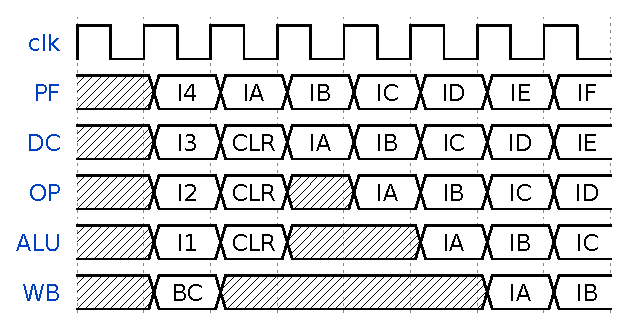
\includegraphics[width=3.5in]{../gfx/bc.eps}
\caption{A conditional branch generates 4 stall cycles}\label{fig:bcstalls}
\end{center}\end{figure}
illustrates the situation for a conditional branch.  In this case, the branch
instruction, {\tt BC}, is nominally followed by instructions {\tt I1} and so
forth.  However, since the branch is taken, the next instruction must be
{\tt IA}.  Therefore, the pipeline needs to be cleared and reloaded.
Given that there are five stages to the pipeline, that accounts
for the four stalls.  (Were the {\tt pipefetch} cache chosen, there would
be another stall internal to the {\tt pipefetch} cache.)

The decode stage can handle the {\tt ADD \$X,PC}, {\tt LDI \$X,PC}, and
{\tt LW (PC),PC} instructions specially, however, when {\tt EARLY\_BRANCHING}
is enabled.  These instructions, when
not conditioned on the flags, can execute with only a single stall cycle (two
for the {\tt LW(PC),PC} instruction),
such as is shown in Fig.~\ref{fig:branch}.
\begin{figure}\begin{center}
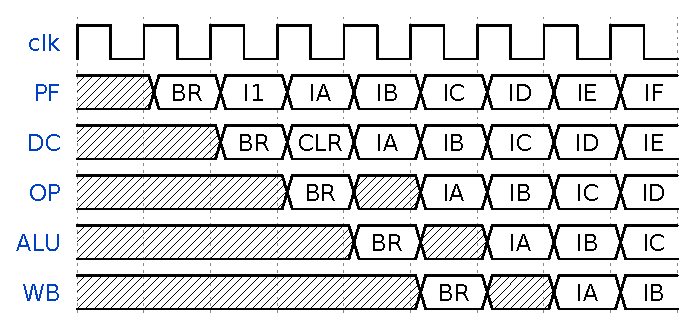
\includegraphics[width=4in]{../gfx/bra.eps} %0.4in per clock
\caption{An expedited branch costs a single stall cycle}\label{fig:branch}
\end{center}\end{figure}
In this example, {\tt BR} is a branch always taken, {\tt I1} is the instruction
following the branch in memory, while {\tt IA} is the first instruction at the
branch address.  ({\tt CLR} denotes a clear--pipeline operation, and does
not represent any instruction.)

\item When reading from a prior register while also adding an immediate offset
\begin{enumerate}
\item\ {\tt OPCODE ?,RA}
\item\ {\em (stall)}
\item\ {\tt OPCODE I+RA,RB}
\end{enumerate}

Since the addition of the immediate register within OpB decoding gets applied
during the read operand stage so that it can be nicely settled before the ALU,
any instruction that will write back an operand must be separated from the
opcode that will read and apply an immediate offset by one instruction.  The
good news is that this stall can easily be mitigated by proper scheduling.
That is, any instruction that does not add an immediate to {\tt RA} may be
scheduled into the stall slot.

This is also the reason why, when setting up a stack frame, the top of the
stack frame is used first: it eliminates this stall cycle.\footnote{This only
applies if there is no local memory to allocate on the stack as well.}  Hence,
to save registers at the top of a procedure, one would write:
\begin{enumerate}
\item\ {\tt SUB 16,SP}
\item\ {\tt SW R1,(SP)}
\item\ {\tt SW R2,4(SP)}
\end{enumerate}
Had {\tt R1} instead been stored at {\tt 1(SP)} as the top of the stack,
there would've been an extra stall in setting up the stack frame.

\item When reading from the CC register after setting the flags
\begin{enumerate}
\item\ {\tt ALUOP RA,RB} {\em ; Ex: a compare opcode}
\item\ {\em (stall)}
\item\ {\tt TST sys.ccv,CC}
\item\ {\tt BZ somewhere}
\end{enumerate}

The reason for this stall is simply performance: many of the flags are
determined via combinatorial logic {\em during} the writeback cycle.
Trying to then place these into the input for one of the operands for an
ALU instruction during the same cycle
created a time delay loop that would no longer execute in a single 100~MHz
clock cycle.  (The time delay of the multiply within the ALU wasn't helping
either \ldots). 

This stall may be eliminated via proper scheduling, by placing an instruction
that does not set flags in between the ALU operation and the instruction
that references the CC register.  For example, {\tt MOV \$addr+PC,uPC}
followed by an {\tt RTU} ({\tt OR \$GIE,CC}) instruction will not incur
this stall, whereas an {\tt OR \$BREAKEN,CC} followed by an {\tt OR \$STEP,CC}
will incur the stall, while a {\tt LDI \$BREAKEN|\$STEP,CC} will not since
it doesn't read the condition codes before executing.

\item When waiting for a memory read operation to complete
\begin{enumerate}
\item\ {\tt LW address,RA}
\item\ {\em (multiple stalls, bus dependent, 4 clocks best)}
\item\ {\tt OPCODE I+RA,RB}
\end{enumerate}

Remember, the ZipCPU does not support out of order execution.  Therefore,
anytime the memory unit becomes busy both the memory unit and the ALU must
stall until the memory unit is cleared.  This is illustrated in
Fig.~\ref{fig:memrd},
\begin{figure}\begin{center}
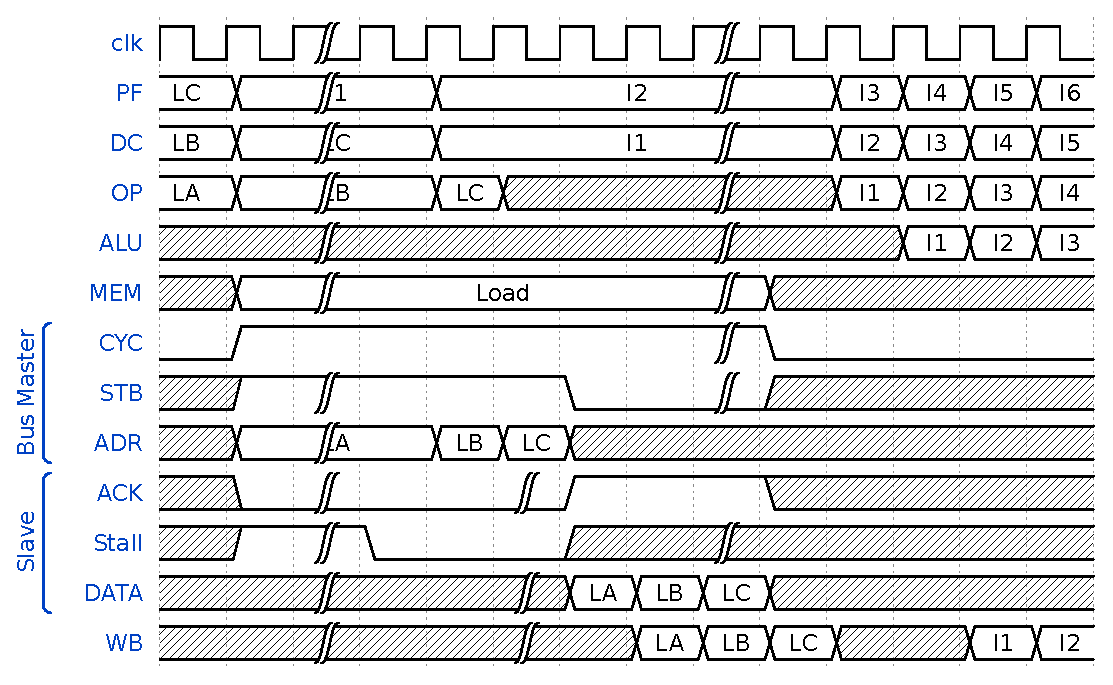
\includegraphics[width=5.6in]{../gfx/memrd.eps}
\caption{Pipeline handling of a load instruction}\label{fig:memrd}
\end{center}\end{figure}
since it is especially true of a load
instruction, which must still write its operand back to the register file.
Further, note that on a pipelined memory operation, the instruction must
stall in the decode operand stage, lest it try to read a result from the
register file before the load result has been written to it.  Finally, note
that there is an extra stall at the end of the memory cycle, so that
the memory unit will be idle for two clocks before an instruction will be
accepted into the ALU.  Store instructions are different, as shown in
Fig.~\ref{fig:memwr},
\begin{figure}\begin{center}
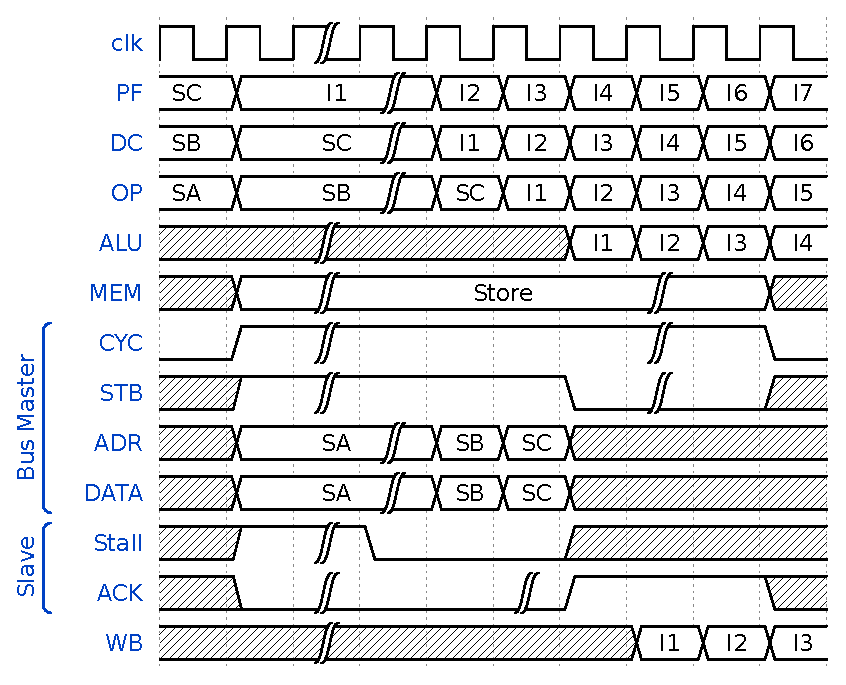
\includegraphics[width=4in]{../gfx/memwr.eps}
\caption{Pipeline handling of a store instruction}\label{fig:memwr}
\end{center}\end{figure}
since they can be busy with the bus without impacting later write back
pipeline stages.  Hence, only loads stall the pipeline.

This, of course, also assumes that the memory being accessed is a single cycle
memory and that there are no stalls to get to the memory.
Slower memories, such as the Quad SPI flash, will take longer--perhaps even
as long as forty clocks.   During this time the CPU and the external bus 
will be busy, and unable to do anything else.  Likewise, if it takes a couple
of clock cycles for the bus to be free, as shown in both Figs.~\ref{fig:memrd}
and~\ref{fig:memwr}, there will be stalls.

\item Memory operation followed by a memory operation
\begin{enumerate}
\item\ {\tt SW address,RA}
\item\ {\em (multiple stalls, bus dependent, 4 clocks best)}
\item\ {\tt LW address,RB}
\item\ {\em (multiple stalls, bus dependent, 4 clocks best)}
\end{enumerate}

In this case, the LW instruction cannot start until the SW is finished,
as illustrated by Fig.~\ref{fig:mstld}.
\begin{figure}\begin{center}
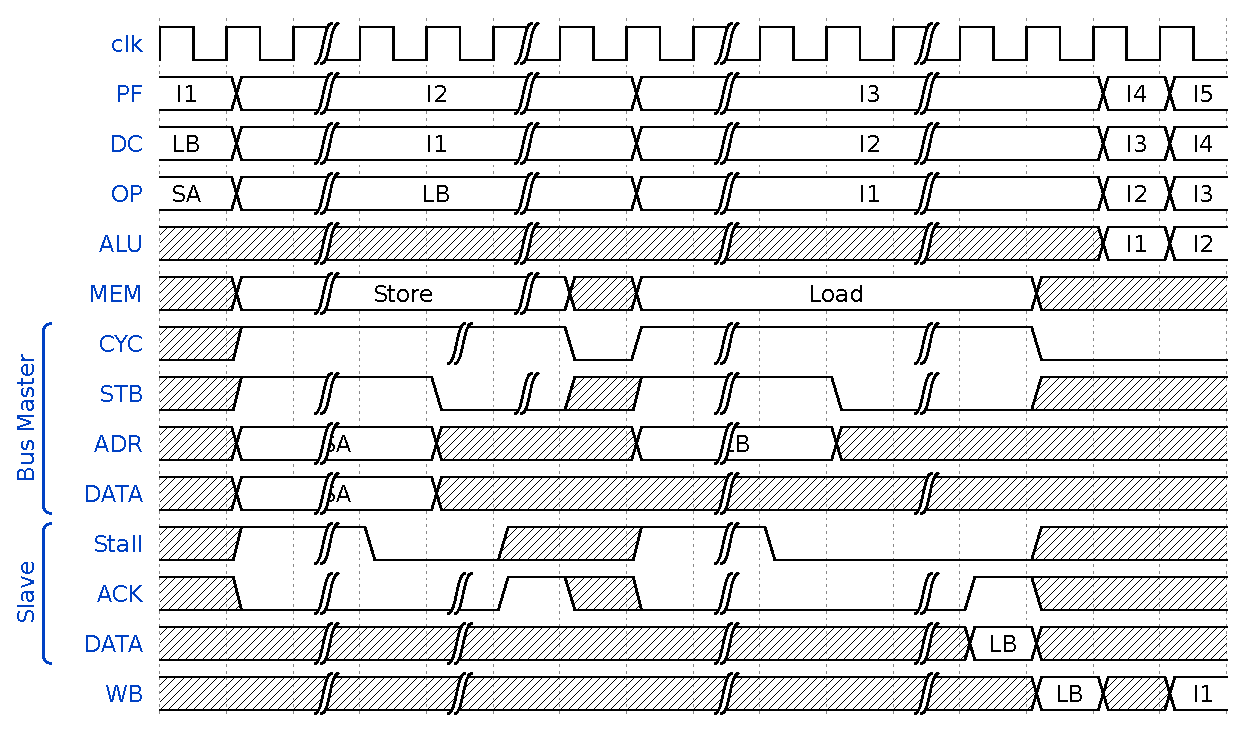
\includegraphics[width=5.5in]{../gfx/mstld.eps}
\caption{Pipeline handling of a store followed by a load instruction}\label{fig:mstld}
\end{center}\end{figure}
With proper scheduling, it is possible to do something in the ALU while the
memory unit is busy with the SW instruction, but otherwise this pipeline will
stall while waiting for it to complete before the load instruction can
start.

The ZipCPU has the capability of supporting a form of burst memory access,
often called pipelined memory access within this document due to its use of
the Wishbone B4 pipelined access mode.
When using this mode, the CPU may issue multiple loads or stores at a time,
to the extent that all but the first take only a single clock.  Doing this
requires several conditions to be true:
\begin{enumerate}
\item Aall accesses within the burst must all be reads or all be writes,
\item All must use the same base register for their address, and
\item There can be no stalls or other instructions between memory access instructions within the burst. 
\item Further, the immediate offset to memory must be either indentical or
	increasing by one address each instruction. 
\end{enumerate}
These conditions work well for saving or storing registers to the stack in a 
burst operation.  Indeed, if you noticed, both Fig.~\ref{fig:memrd} and
Fig.~\ref{fig:memwr} illustrated pipelined memory accesses.  Beyond saving and
restoring registers to the stack, the compiler does not optimize well (yet)
for using this burst mode.

\end{itemize}

% \subsection{Debug}

\section{External Architecture}

Having now described the CPU registers, instructions, and instruction formats,
we now turn our attention to how the CPU interacts with the rest of the world.
Specifically, we shall discuss how the bus is implemented, and the memory
model assumed by the CPU.

\subsection{Simplified Wishbone Bus}\label{ssec:bus}
The bus architecture of the ZipCPU is that of a simplified, pipelined, WISHBONE
bus built according to the B4 specification.  Several changes have been made to
simplify this bus.  First, all unnecessary ancillary information has been
removed.  This includes the retry, tag, lock, cycle type indicator, and burst
indicator signals.  The bus supports big endian operation where the high order
octet occupies the low order address.  Second, we insist that all
accesses be pipelined, and simplify that further by insisting that pipelined
accesses not cross peripherals---although we leave it to the user to keep that
from happening in practice.  Finally, we insist that the wishbone strobe line
be zero any time the cycle line is inactive.  This makes decoding simpler
in slave logic: a transaction is initiated whenever the strobe line is high
and the stall line is low.  For those peripherals that do not generate stalls,
only the strobe line needs to be tested for access.  The transaction completes
whenever either the ACK or the ERR lines go high.

\subsection{Memory Model}\label{ssec:memory}
The memory model of the ZipCPU is that of a uniform 32--bit address space.
The CPU knows nothing about which addresses reference on--chip or off-chip
memory, or even which reference peripherals.  Indeed, there is no indication
within the CPU if a particular piece of memory can be cached or not, save that
the CPU assumes any and all instruction words can be cached.

The one exception to this rule revolves around addresses where the top 8-bits
of their high order word are all ones.  These addresses are used to access a
variety of optional peripherals that will be discussed more in
Sec.~\ref{sec:zipsys}, but that are only present within the {\tt ZipSystem}.
When used with the bare {\tt ZipBones}, these addresses will cause a bus error.

The prefetch cache currently has no means of detecting an instruction that
was changed, save by clearing the instruction cache.  This may be necessary
when loading programs into previously used memory, or when creating
self--modifying code.

Should the memory management unit (MMU) be integrated into the ZipCPU, the MMU
configuration will tell the ZipCPU wich addresses may be cached and which not.

This topic is discussed further in the linker section, Sec.~\ref{sec:ld-mem}
of the ABI chapter, Chap.~\ref{chap:abi}.

% \subsection{Measured Performance}\label{sec:perf}

\subsection{ZipSystem}\label{sec:zipsys}

While the previous chapter describes a CPU in isolation, the ZipSystem
includes a small minimum set of peripherals that can be tightly integrated into
the CPU.  These peripherals are shown in Fig.~\ref{fig:zipsystem}
\begin{figure}\begin{center}
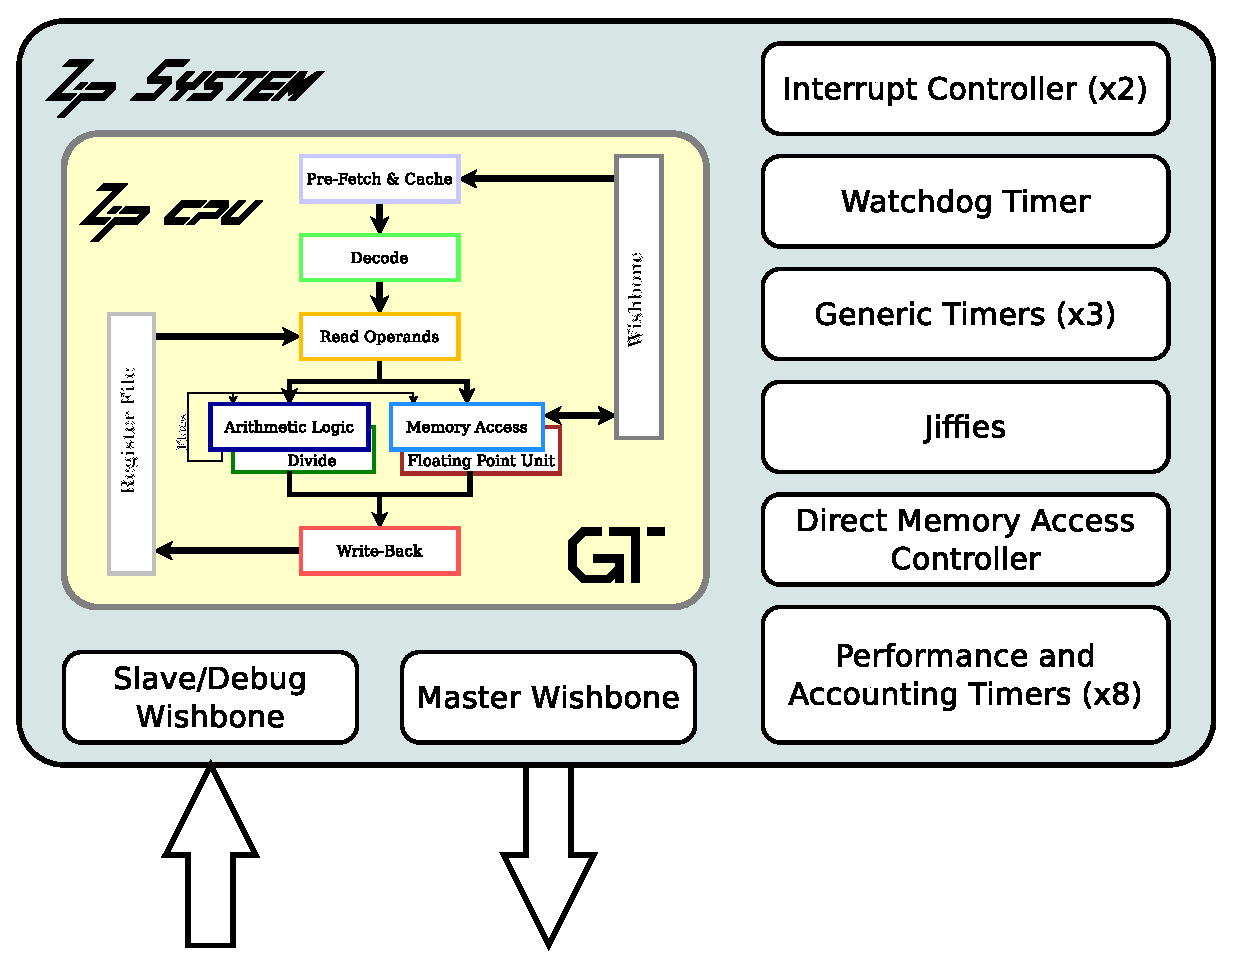
\includegraphics[width=3.5in]{../gfx/system.eps}
\caption{ZipSystem Peripherals}\label{fig:zipsystem}
\end{center}\end{figure}
and described here.  They are designed to make
the ZipCPU more useful in an Embedded Operating System environment.

\subsubsection{Interrupt Controller}\label{sec:pic}

Perhaps the most important peripheral within the ZipSystem is the interrupt
controller.  While the ZipCPU itself can only handle one interrupt, and has
only the one interrupt state: disabled or enabled, the interrupt controller
can make things more interesting.

The ZipSystem interrupt controller module supports up to 15 interrupts, all
controlled from one register.  Further, it has been designed so that individual
interrupts can be enabled or disabled individually without having any knowledge
of the rest of the controller setting.  To enable an interrupt, write to the
register with the high order global enable bit set and the respective interrupt
enable bit set.  No other bits will be affected.  To disable an interrupt,
write to the register with the high order global enable bit cleared and the
respective interrupt enable bit set.  To clear an interrupt, write a `1' to
that interrupt's status pin.  A zero written to the register has the sole
effect of disabling the master interrupt enable bit.

As an example, suppose you wished to enable interrupt \#4.  You would then
write to the register a {\tt 0x80100010} to enable interrupt \#4 and to clear
any past active state.  When you later wish to disable this interrupt, you would
write a {\tt 0x00100010} to the register.  This both disables the
interrupt and clears the active indicator.  This also has the side effect of
disabling all interrupts, so a second write of {\tt 0x80000000} may be necessary
to re-enable any other interrupts.

The ZipSystem hosts two interrupt controllers: a primary and a secondary.  The
primary interrupt controller is the one that interrupts the CPU.  It has
six local interrupt lines, the rest coming from external interrupt sources.
One of those interrupt lines to the primary controller comes from the secondary
interrupt controller.  This controller maintains an interrupt state for the
process accounting counters, and any other external interrupts that didn't fit
into the primary interrupt controller.

As a word of caution, because the interrupt controller is an external
peripheral, and because memory writes take place concurrently with any following
instructions, any attempt to clear interrupts on one instruction followed by
an immediate Return to Userspace ({\tt RTU}) instruction, may not have the
effect of having interrupts cleared before the {\tt RTU} instruction executes.

\subsubsection{Counter}

The Zip Counter is a very simple counter: it just counts.  It cannot be
halted.  When it rolls over, it issues an interrupt.  Writing a value to the
counter just sets the current value, and it starts counting again from that
value.

Eight counters are implemented in the ZipSystem for process accounting if
the {\tt INCLUDE\_ACCOUNTING\_COUNTERS} define is set within {\tt cpudefs.v}.
Four of those measure the performance of the system as a whole, four are
used for measuring user CPU usage.
This may change in the future, as nothing as yet uses these counters.

\subsubsection{Timer}

The Zip Timer is also very simple: it is a 31--bit counter that simply counts
down to zero.  When it transitions from a one to a zero it creates an interrupt.

Writing any non-zero value to the timer starts the timer.  If the high order
bit is set when writing to the timer, the timer becomes an interval timer and
reloads its last start time on any interrupt.  Hence, to mark seconds, one
might set the 31--bits of the timer to the number of clocks per second and the
top bit to one.  Ever after, the timer will interrupt the CPU once per
second--until a non--interrupt interval is set in the timer.  This reload
capability also limits the maximum timer value to $2^{31}-1$, rather than
$2^{32}-1$.

\subsubsection{Watchdog Timer}

The watchdog timer has only two differences from the of the other timers.
The first difference is that it is a one--shot timer.  The second difference,
though, is critical: the interrupt line from the watchdog timer is tied to the
reset line of the CPU.  Hence writing a `1' to the watchdog timer will always
reset the CPU.  To stop the Watchdog timer, write a `0' to it.  To start it,
write any other number to it---as with the other timers.


\subsubsection{Bus Watchdog}
There is an additional watchdog timer on the Wishbone bus of the ZipSystem. 
This timer,
however, is hardware configured and not software configured.  The timer is
reset at the beginning of any bus transaction, and only counts clocks during
such bus transactions.  If the bus transaction takes longer than the number
of counts the timer allots, it will raise a bus error flag to terminate the
transaction.  This is useful in the case of any peripherals that are
misbehaving.  If the bus watchdog terminates a bus transaction, the CPU may
then read from its port to find out which memory location created the problem.

Aside from its unusual configuration, the bus watchdog is just another
implementation of the fundamental timer described above--stripped down
for simplicity.

\subsubsection{Jiffies}

This peripheral is motivated by the Linux use of `jiffies' whereby a process
can request to be put to sleep until a certain number of `jiffies' have
elapsed.  Using this interface, the CPU can read the number of `jiffies'
from the peripheral (it only has the one location in address space), add the
sleep length to it, and write the result back to the peripheral.  The
{\tt zipjiffies}
peripheral will record the value written to it only if it is nearer the current
counter value than the last current waiting interrupt time.  If no other 
interrupts are waiting, and this time is in the future, it will be enabled.
(There is currently no way to disable a jiffie interrupt once set, other
than to disable the interrupt line in the interrupt controller.)  The processor
may then place this sleep request into a list among other sleep requests.
Once the timer expires, it would write the next Jiffy request to the peripheral
and wake up the process whose timer had expired.

Indeed, the Jiffies register is nothing more than a glorified counter with
an interrupt.  Unlike the other counters, the internal Jiffies counter can only
be read, never set.
Writes to the jiffies register create an interrupt time.  When the Jiffies
register later equals the value written to it, an interrupt will be asserted
and the register then continues counting as though no interrupt had taken
place.

Finally, if the new value written to the Jiffies register is within the past
$2^{31-1}$ clock ticks, the Jiffies register will immediately cause an interrupt
and otherwise ignore the new request.

The purpose of this register is to support alarm times within a CPU.  To
set an alarm for a particular process $N$ clocks in advance, read the current
Jiffies value, add $N$, and write it back to the Jiffies register.  The
O/S must also keep track of values written to the Jiffies register.  Thus,
when an `alarm' trips, it should be removed from the list of alarms, the list
should be resorted, and the next alarm in terms of Jiffies should be written
to the register--possibly for a second time.

\subsubsection{Direct Memory Access Controller}

The Direct Memory Access (DMA) controller can be used to either move memory
from one location to another, to read from a peripheral into memory, or to
write from a peripheral into memory all without CPU intervention.  Further,
since the DMA controller can issue (and does issue) pipeline wishbone accesses,
any DMA memory move will by nature be faster than a corresponding program
accomplishing the same move.  To put this to numbers, it may take a program
running on the CPU 18~clocks per word transferred, whereas this DMA controller
can move one word in eight clocks--provided it has bus
access\footnote{The pipeline cost of the DMA controller, including setup cost,
is a minimum of $14+2N$ clocks.} (The CPU gets priority over the bus, but once
bus access is granted to the DMA peripheral, it will not be revoked mid--read
or mid--write.)

The DMA controller supports only aligned word accesses.  It does not support
byte or half-word accesses.

When copying memory from one location to another, the DMA controller will
copy in units of a given transfer length--up to 1024 words at a time.  It will
read that transfer length into its internal buffer, and then write to the
destination address from that buffer.

When coupled with a peripheral, the DMA controller can be configured to start
a memory copy when any interrupt line goes high.  Further, the controller can
be configured to issue reads from (or to) the same address instead of
incrementing the address at each clock.  The DMA completes once the total
number of items specified (not the transfer length) have been transferred.

In each case, once the transfer is complete and the DMA unit returns to
idle, the DMA will issue an interrupt.

% \subsubsection{Memory Management Unit}

\section{Debug Interface}\label{sec:debug}

The ZipCPU supports an external debug port.  Access to the port is the
same as accessing a two register peripheral on a wishbone bus, so the basic
interface is fairly simple.  Using this interface, it is possible to both
control the CPU, as well as read register values and current status from the
CPU.

While a more detailed discussion will be reserved for Sec.~\ref{sec:reg-debug},
here we'll just discuss how it is put together.  The debug interface allows
a controller access to the CPU reset line, and a halt line.  By raising the
reset line, the CPU will be caused to clear it's cache, to clear any internal
exception or error conditions, and then to start execution at the
{\tt RESET\_ADDRESS}--just like a normal reboot.  In a similar fashion, the
debug interface allows you to control the {\tt cpu\_halt} line into the
CPU.  Holding this line high will hold the CPU in an externally halted state.
Toggling the line low for one clock allows one to step the CPU by one 
instruction.  Lowering the line causes the CPU to go.  A final control wire, 
controlled by the debug interface, will force the CPU to clear its cache.
All of these control wires are set or cleared from the debug control register.

The two debug command registers also make it possible to read and write
all 32 registers within the CPU.  In this fashion, a debugger can halt the
CPU, investigate its state, and even modify registers so as to have the
CPU restart from a different state.

Finally, without halting the CPU, the debug controller can read from any
single register, and it can see if the CPU is still actively running, whether
it is in user or supervisor modes, and whether or not it is sleeping.  This
alone is useful for detecting deadlocks or other difficult problems.

\chapter{Application Binary Interface}\label{chap:abi}

This chapter discusses not the CPU itself, but rather how the GCC and binutils
toolchains have been configured to support the ZipCPU.

% ELF Format
% Stack:
%	R13 is the stack register.
%	The stack grows downward.
%	Memory at the current stack pointer is allocated.
%	Hence, a PUSH is : SUB 1,SP; SW Rx,(SP)
% Heap:
%	In general, not yet implemented.  
%	A less than adequate Heap has been implemented as a pointer, from which
%	malloc requests simply decrement it.  Free's are NOOPs, leaving
%	allocated memory allocated forever.

\section{Executable File Format}\label{sec:abi-elf}
ZipCPU executable files are stored in the Executable and Linkable Format
(ELF), prior to being placed in flash, or whatever memory they will be
executed from.  

The ZipCPU described by this specification uses the 16-bits {\tt 16'hdad1}
to identify itself against other CPUs.  This is not an officially registered
number, and may change in the future.

The ZipCPU does not (yet) have a dynamic linker/loader.  All linking is
currently static, and done prior to run time.

\section{Stack}\label{sec:abi-stack}
Register {\tt R13} (also known as the {\tt SP} register) is the stack register.
The compiler generates code that grows the stack from
high addresses to lower addresses.  That means that the stack will usually
start out set to a very large value, such as one past the last RAM address,
and it will grow to lower and lower values--hopefully never mixing with the
heap.  Memory at the current stack position is assumed to be allocated.

When creating a stack frame for a function, the compiler will subtract
the size of the stack frame from the stack register.  It will then store
any registers used by the function, from {\tt R5} to {\tt R12} (including
the link register {\tt R0}) onto offsets given by the stack pointer plus a 
constant.  If a frame pointer is used, the compiler uses {\tt R12} (or
{\tt FP}) for this purpose.  The frame pointer is set by moving the stack
pointer plus an offset into {\tt FP}.  This {\tt MOV} instruction effectively
limits the size of any individual stack frame to $2^{12}-1$ octets.

Once a subroutine is complete, the frame is unwound.  If the frame pointer,
{\tt FP} was used, then {\tt FP} is copied directly to the stack pointer,
{\tt SP}.  Registers are restored, starting with {\tt R0} all the way to
{\tt R12} ({\tt FP}).  This also restores, and obliterates, the subroutine
frame pointer.  Once complete, a value is added to the stack pointer to
return it to its original value, and a jump is made to the value located
within {\tt R0}.

\section{Relocations}\label{sec:abi-reloc}

The ZipCPU binutils back end supports several types of relocations, although
the two most common are the 32--bit relocations for register load and long
jump.

The first of these is for loading an arbitrary 32--bit value into a register. 
Such instructions are broken into a pair of {\tt BREV} and {\tt LDILO}
instructions, and once the value of the parameter is known their immediate
values can be filled in.

The second type of 32--bit relocation is for jumps to arbitrary addresses.
These jumps are supported by the \hbox{\tt LW (PC),PC} instruction, followed
by the 32--bit address to be filled in later by the linker.  If the jump is
conditional, then a conditional \hbox{\tt LW.$x$ 4(PC),PC} instruction is
used, followed by a {\tt ADD 4,PC} and then the 32--bit relocation value.

If a branch distance is known and within reach, then it will be implemented
with an {\tt ADD \#,PC} instruction, possibly conditional, as necessary.

While other relocations are supported, they tend not to be used nearly as much
as these two.

\section{Call format}\label{sec:abi-jsr}

One unique of the ZipCPU is that it has no JSR instruction.  The assembler
attempts to minimize this problem by replacing a {\tt JSR}~{\em address}
instruction with a {\tt MOV \#(PC),R0} followed by a jump to the requested
address.  In this case, the offset to the PC for the {\tt MOV} instruction
is determined by whether or not the jump can be accomplished with a local
branch or a long jump.

While this works well in practice, this implementation prevents such things
as {\tt JSR}'s followed by {\tt BRA}'s from being combined together.

Finally, GCC will place first five operands passed to the subroutine into
registers R1--R5.  Any additional operands are placed upon the stack.

\section{Built-ins}\label{sec:abi-builtin}
The ZipCPU ABI supports the a number of built in functions.  The compiler
maps these functions directly to assembly language equivalents, essentially 
providing the C~programmer with access to several assembly language
instructions.  These are:
\begin{enumerate}
\item {\tt zip\_bitrev(int)} reverses the bits in the given integer, returning
	the result.  This utilizes the internal {\tt BREV} instruction, and is
	designed to be used with FFT's as necessary.
\item {\tt zip\_busy()} executes an {\tt ADD -4,PC} function, essentially
	forcing the CPU into a very tight infinite loop.
\item {\tt zip\_cc()} returns the value of the current CC register.  This may
	be used within both user and supervisor code to determine in which
	mode the CPU is within.
\item {\tt zip\_halt()} executes an \hbox{\tt OR \$SLEEP,CC} instruction to
	place the processor to sleep.  If the processor is in supervisor mode,
	this halt's the processor.
\item {\tt zip\_rtu()} executes an \hbox{\tt OR \$GIE,CC} instruction.  This
	will place the CPU into user mode, and has no effect if the CPU is
	already in user mode.
\item {\tt zip\_step()} executes an \hbox{\tt OR \$STEP|\$GIE,CC} instruction.
	This will place the CPU into user mode in order to step one instruction,
	and then return to supervisor mode.
	It has no effect if the CPU is already in user mode.
\item {\tt zip\_system()} executes an \hbox{\tt AND \textasciitilde\$GIE,CC}
	instruction to return the CPU to supervisor mode.  This essentially
	executes a trap, setting the trap bit for the supervisor to examine. 
	What this instruction does not do is arrange for the trap arguments to
	be placed into the  registers {\tt R1} through {\tt R5}.  Since this is
	a wholly inadequate solution, a function call may be made to an
	assembly routine that executes a trap if necessary.
\item {\tt zip\_wait()} executes a \hbox{\tt \$SLEEP|\$GIE,CC} instruction.
	Unlike {\tt zip\_halt()}, this {\tt zip\_wait()} instruction places
	the CPU into a wait state regardless of whether or not the CPU is
	in supervisor mode or not.   When this function, i.e. instruction,
	completes, it will leave the CPU in supervisor mode upon an interrupt
	having taken place.

	You may wish to set the user program counter prior to this instruction,
	as the prefetch unit will try to load instructions from the address
	contained within the user program counter.  Attempts to read from 
	addresses with sideeffects may not produce the desired outcome. 
	However, once that cache fails (or succeeds), the CPU will have been
	put to sleep and will do no more.

\item {\tt zip\_restore\_context(context *)} inserts the 32~assembly
	instructions necessary to copy all sixteen user registers to a memory
	region pointed to by the given context pointer, starting with {\tt uR0}
	on up to {\tt uPC}.

\item {\tt zip\_save\_context(context *)} inserts the 32~assembly instructions
	necessary to copy all sixteen user registers to a memory region pointed
	to by the given context pointer argument, starting
	with {\tt uR0} on up to {\tt uPC}.
\item {\tt zip\_ucc()}, returns the value of the user CC register.
\end{enumerate}

% Builtin functions:
%	zip_break();
%	zip_idle();
%	zip_syscall(a,b,c,d)
%
\section{Linker Scripts}\label{sec:ld}
The ZipCPU makes no assumptions about its memory layout.  The result, though,
is that the memory layout of a given project is board specific.  This
is accomplished via a board specific linker script.  This section will discuss
some of the specifics of a ZipCPU linker script.

Because the ZipCPU uses a modified binutils package as part of its tool chain,
the format for this linker script is defined by the GNU LD project within
binutils.  Further details on that format may be found within the GNU LD 
documentation within the binutils package.

This discussion will focus on those parts of the script specific to the ZipCPU.

\subsection{Memory Types}\label{sec:ld-mem}
Of the FPGA boards that the ZipCPU has been applied to, most of them have some
combination of three types of memory: flash, block RAM, and Synchronous 
Dynamic RAM (SDRAM).  Of these three, only the flash is non--volatile.  The
block RAM is the fastest, and the SDRAM the largest.  While other memory types
are available, such as files on an external media such as an SD card or a 
network drive, these three types have so far been sufficient for our purposes.

To support these memories, the linker script has three memory lines identifying
where each memory exists on the bus, the size of the memory, and any protections
associated with it.  For example,
\begin{eqnarray*}
\mbox{blkram (wx) : ORIGIN = 0x0008000, LENGTH = 0x0008000}
\end{eqnarray*}
specifies that there is a region of memory, called blkram, that can be read and
written, and that programs can execute from.  This section starts at address
{\tt 0x8000} and extends for another {\tt 0x8000} bytes.  The other memories
are defined in a similar manner, with names {\tt flash} and {\tt sdram}.

Following the memory section, three specific symbols are defined:
	{\tt \_flash}, defining the beginning of flash memory,
	{\tt \_blkram}, defining the beginning of on--chip block RAM,
	and
	{\tt \_sdram}, defining the beginning of SDRAM.
These symbols are used to make the bootloader's task easier.

\subsection{The Entry Function}\label{sec:ld-entry}
The ZipCPU has, as a parameter, a {\tt RESET\_ADDRESS}.  It is important
that this address contain a valid instruction (or more), since this is the
first instruction the ZipCPU will execute.  Traditionally, this address is also
the first address in instruction memory as well.

To make this happen, the ZipCPU defines two additional segments: the
{\tt .start} and the {\tt .boot} segments.  The {\tt  .start} segment is to 
have nothing in it but the very initial startup code.  This code needs to run 
from flash (or other ROM).  By placing this segment at the very beginning of
the ZipCPU's flash address space, and in particular at the first valid flash
address, the ZipCPU will boot from this address.  This is the purpose of the
{\tt .start} section.

The {\tt .boot} section has a similar purpose.  This section includes anything
associated with the bootloader.  It is a special section because, when loading
from flash, the bootloader {\em cannot} be placed in RAM, but must be placed
in flash--since it is the code that loads things from flash into RAM.

It may also make sense to place any code executed once only within flash as
well.  Such code may run slower than the main system code, but by leaving it in
flash it can be kept from consuming any higher speed RAM.  To do this, place
this other code into the {\tt .boot} section.

You may also find that large data structures that are best left in flash
can also be placed into this {\tt .boot} section as well for that purpose.

\subsection{Bootloader Tags}\label{sec:ld-boot}

The bootloader needs to know a couple things from the linker script.  It needs
to know what code/data to copy to block RAM from the flash, what code/data to
copy to SDRAM, and finally what initial data area needs to be zeroed.  Four
additional pointers, set within a linker script, can define these regions.

\begin{enumerate}
\item {\tt \_kernel\_image\_start}

	This is the first location in flash containing data that the bootloader
	needs to move.

\item {\tt \_kernel\_image\_end}

	This is a pointer to one past the last location in block RAM to place
	things into.  If this pointer is equal to {\tt \_kernel\_image\_start},
	then no information is placed into block RAM.

\item {\tt \_sdram\_image\_start}

	This should be equal to {\tt \_kernel\_image\_end}.  It is a pointer,
	within block RAM address space, of the first location to be moved
	into SDRAM.  By adding the difference between
	{\tt \_sdram\_image\_start} and {\tt \_blkram} to the flash address
	in {\tt \_kernel\_image\_start}, the actual source address within the
	flash of the code/data that needs to be copied into SDRAM can be
	determined.

\item {\tt \_sdram\_image\_end}

	This is the ending address of any code/data to be copied into SDRAM.
	The distance between this pointer and {\tt \_sdram} should be the 
	amount of data to be placed into SDRAM.

\item {\tt \_bss\_image\_end}

	The BSS segment contains data the starts with an initial value of
	zero.  Such data are usually not placed in the executable file, nor
	are they placed into any flash image.  This address points to the
	last location in SDRAM used by the BSS segment.  The bootloader
	is responsible then for clearing the SDRAM between
	{\tt \_sdram\_image\_end} and {\tt \_bss\_image\_end}.

	The bootloader must also be robust enough to handle the cases where
	1) there is no SDRAM, 2) there is no block RAM, and 3) where there
	is non requirement to move memory at all---such as when the program
	is placed into memory and started from there.
\end{enumerate}
\subsection{Other required linker symbols}\label{sec:ld-other}

Two other symbols need to be defined in the linker script, which are used
by the startup code.  These are:
\begin{enumerate}
\item {\tt \_top\_of\_stack}

	This is the address that the startup code will set the stack pointer
	to point to.  It may be one past the last location of a RAM memory,
	whether block RAM or SDRAM.

\item {\tt \_top\_of\_heap}

	This is the first location past the end of the {\tt .bss} segment.
	Equivalently, this is the address of the first unused piece of
	memory, or the location from whence to start any dynamic memory
	subsystem.
\end{enumerate}

All of these symbols need to reference word aligned addresses.

\section{Loading ZipCPU Programs}
There are two basic ways to load a ZipCPU program, depending upon whether or
not the ZipCPU is active within the current configuration.  If the ZipCPU
is not a part of the current FPGA configuration, one need only write the 
flash and then switch configurations.  It will be the CPU's responsibility
to place itself in RAM then. 

The more practical alternative is a little more involved, and there are
several steps to it.
\begin{enumerate}
\item Halt the CPU by writing 0x0440 to the CPU control register.  This
	both halts and resets the CPU.  It then prevents both bus contention,
	while writing the new instructions to memory, as well as preventing the
	CPU from running some instructions from one program and other
	instructions from another.
\item Load the program into memory.  For many programs this will involve
	loading the program into flash, and necessitate having and using a 
	flash controller.  The ZipCPU also supports being loaded straight into
	RAM address as well, as though the bootloader had completed
	it's task.
\item You may optionally, at this point, clear all of the CPUs registers,
	to make certain the reboot is clean.
\item Set the sPC register to the starting address. 
\item Clear the instruction cache in order to force the CPU to reload its
	cache upon start.
\item Release the CPU by writing to the CPU debug control register a number
	between 0 and 31.  This number will correspond to the register number
	of the register that can be ``peeked'' at while the CPU is running.
\end{enumerate}

%
\section{Starting a ZipCPU program}
\subsection{CRT0}

Most computers have a section of code, conventionally called {\tt crt0}, which
loads a program into memory.  On the ZipCPU, this code starts at {\tt \_start}.
It is responsible for setting the stack pointer, calling the boot loader,
and then calling the main entry function, {\tt entry()}.

Because {\tt \_start} {\em must} be the first symbol in a program, and because
that first symbol is located at the boot address for the CPU, the {\tt \_start}
is placed into the {\tt .start} segment.  It is the only routine placed there.

On those CPU's that don't have enough logic space for a debugger, it may be
useful to place a routine to dump any registers, stack values and/or kernel
traces to an output routine at this time.  That way, on any kernel fault, the
kernel can be brought back up with a debug trace.  This works because rebooting
the CPU doesn't reset any register values save the {\tt sCC} and {\tt sPC}.

\subsection{The Bootloader}

As discussed in Sec.~\ref{sec:ld-boot}, the bootloader must be placed into 
flash if it is used.  It can be a small C program (it need not be assembly,
like {\tt \_start}), and it only needs to copy memory.  First, it copies any
memory from flash to block RAM.  Second, it copies any necessary memory from
flash to SDRAM.  Then, it zeros any memory necessary in SDRAM (or block RAM,
if there is no SDRAM).

These memory copies may be done with the DMA, or they may be done one--at--a
time for a performance penalty.

\subsection{Kernel Entry}

After calling the boot loader, execution returns to the {\tt \_start} routine
which then calls the main program entry function, {\tt entry()}.  No
requirements are laid upon this entry function regarding where it must reside.
The simplest place to put it is in Block RAM--and just to put all code and
variables there.  In reality, this entry function may easily be left in flash.
It often doesn't need to run particularly fast, since there may easily be
one--time setup functions that are independent of the programs main loop.

\subsection{Kernel Main}

If the kernel entry function, {\tt entry()}, is placed in flash, it should call
a separate function to run the main while loop once it has been set up.  In
this fashion, the main while loop may be kept in the fastest memory necessary
(that it will fit within), to ensure good performance.

\chapter{Operation}\label{chap:ops}

This chapter will explore how to perform common tasks with the ZipCPU,
offering examples in both C and assembly for those tasks.

\section{CRT0}

Of course, the one task that every CPU must do is start the CPU for other
tasks.  The ZipCPU is no different.  This is the one ZipCPU task that must
take place in assembly, since no assumptions can be made about the state of
the ZipCPU upon entry.  In particular, the stack pointer, SP, needs to be
loaded with a valid memory location before any higher level language can work.
Once that has taken place, it is then possible to call other higher level
routines.

Table.~\ref{tbl:op-init}
\begin{table}\begin{center}
\begin{tabbing}
{\em ; By starting our loader in the .start section, we guarantee through our}\\
{\em ; linker script that these are the very first instructions the CPU sees.}\\
\hbox to 0.25in{}\={\tt .section .start} \\
\>	{\tt .global \_start} \\
{\em ; \_start is to be placed at our reboot/reset address, so it will be}\\
{\em ; called upon any reboot.}\\
{\tt \_start:} \\
\> {\em ; The most important step: creating a stack pointer.  The value}\\
\> {\em ; {\tt \_top\_of\_stack} is created by the linker based upon the linker script.}\\
\>	{\tt LDI \_top\_of\_stack,SP} \\
\> {\em ; We then call the bootloader to load our code into memory.}\\
\>	{\tt MOV \_after\_bootloader(PC),R0} \\
\>	{\tt BRA bootloader} \\
{\tt \_after\_bootloader:} \\
\>	{\em ; Just in case the bootloader messed up the stack, we'll reset it here.}\\
\>	{\tt LDI \_top\_of\_stack,SP} \\
\>	{\em ; Finally, we call the entry function for the entire design.}\\
\>	{\tt MOV \_kernel\_exit(PC),R0}\\
\>	{\tt BRA entry}\\
{\em ; The {\tt \_kernel\_exit} routine that follows isn't strictly necessary,}\\
{\em ; since the CPU should never return from the {\tt entry()} function.  However,}\\
{\em ; since returning from such a function is valid C code, and just in case}\\
{\em ; it does return, we provide this function as a fail safe to make sure}\\
{\em ; the kernel halts upon completion.}\\
{\tt \_kernel\_exit:}\\
\> {\tt HALT}\\
\> {\tt BRA \_kernel\_exit}
\end{tabbing}
\caption{Setting up a stack frame and starting the CPU}\label{tbl:op-init}
\end{center}\end{table}
presents an example of one such initialization routine
that first sets up the stack, then calls a bootloader routine.  Upon completion,
the initialization routine then calls the main entry point for the CPU.  Should
that main entry point ever return, a short routine following halts the CPU.

The example also highlights one optimization that didn't take place.  Instead
of placing the {\tt \_after\_bootloader} address into {\tt R0}, this script
could have placed the {\tt entry()} address into {\tt R0}.  Had it done so, the
CPU would not have suffered the pipeline stalls associated with two long jumps:
the first to {\tt R0}, and the second to {\tt entry}.  Instead, it would have
suffered such stalls only once: when jumping to {\tt entry()}.

% \section{Example bootloader}

\section{System High}
The easiest and simplest way to run the ZipCPU is in the system high mode.
In this mode, the CPU runs your program in supervisor mode from reboot to
power down, and is never interrupted.  You will need to poll the interrupt
controller to determine when any external condition has become active.  This
mode is incredibly useful, and can handle many microcontroller--type tasks. 

Even better, in system high mode, all of the user registers are available
to the system high program as variables.  Accessing these registers can be
done in a single clock cycle, which would move them to the active register
set or move them back.  While this may seem like a load or store instruction,
none of these register accesses will suffer from memory delays.

The one thing that cannot be done in supervisor mode is a wait for interrupt
instruction.  This, however, is easily rectified by jumping to a user task
within the supervisors memory space, such as Tbl.~\ref{tbl:shi-idle}.
\begin{table}\begin{center}
\begin{tabbing}
{\tt supervisor\_idle:} \\
\hbox to 0.25in{}\={\em ; While not strictly required, the following move helps to} \\
\>	{\em ; ensure that the prefetch doesn't try to fetch an instruction} \\
\>	{\em ; outside of the CPU's address space when it switches to user} \\
\>	{\em ; mode.} \\
\>	{\tt MOV supervisor\_idle\_continue,uPC} \\
\>	{\em ; Put the processor into user mode and to sleep in the same} \\
\>	{\em ; instruction. } \\
\>	{\tt OR \$SLEEP|\$GIE,CC} \\
{\tt supervisor\_idle\_continue:} \\
\>	{\em ; Now, if we haven't done this inline, we need to return} \\
\>	{\em ; to whatever function called us.} \\
\>	{\tt RETN} \\
\end{tabbing}
\caption{Executing an idle from supervisor mode}\label{tbl:shi-idle}
\end{center}\end{table}

There are some problems with this model, however.  For example, even though
the user registers can be accessed in a single cycle, there is currently
no way to do so other than with assembly instructions.

An alternative to this approach is to use the {\tt zip\_wait()} built--in
function.  This places the ZipCPU into an idle/sleep mode to wait for
interrupts.  Because the supervisor puts the CPU to sleep, rather than the
user, no user context needs to be set up.

\section{A Programmable Delay}

One common task in microcontrollers, whether in a user task or supervisor
task, is to wait for a programmable amount of time.  Using the ZipSystem,
there are several peripherals that can be used to create such a delay.
It can be done with one of the three timers, the jiffies, or even an off-chip
ZipCounter.

Here, in Tbl.~\ref{tbl:shi-timer},
\begin{table}\begin{center}
\begin{tabbing}
{\tt \#define EINT(A) (0x80000000|(A<<16))} \= {\em // Enable interrupt A}\\
{\tt \#define DINT(A) (A<<16)} \>{\em // Just disable the interrupts in A}\\
{\tt \#define DISABLEALL 0x7fff0000} \>{\em // Disable all interrupts}\\
{\tt \#define CLEARPIC 0x7fff7fff} \>{\em // Clears and disables all interrupts}\\
{\tt \#define SYSINT\_TMA 0x10} \>{\em // The Timer--A interrupt mask}\\
\\
{\tt void timer\_delay(int nclocks) \{} \\
\hbox to 0.25in{}\= {\em // Clear the PIC.  We want to exit from here on timer counts alone}\\
	\> {\tt zip->pic = DISABLEALL|SYSINT\_TMA;}\\
	\> {\tt if (nclocks > 10) \{}\\
	\> \hbox to 0.25in{}\= {\em // Set our timer to count down the given number of counts}\\
	\> \> {\tt zip->tma = nclocks;} \\
	\> \> {\tt zip->pic = EINT(SYSINT\_TMA);} \\
	\> \> {\tt zip\_wait();} \\
	\> \> {\tt zip->pic = CLEARPIC;} \\
	\> {\tt \} }{\em // else anything less has likely already passed} \\
{\tt \}}\\
\end{tabbing}
\caption{Waiting on a timer}\label{tbl:shi-timer}
\end{center}\end{table}
we present one means of waiting for a programmable amount of time using a
timer.  If exact timing is important, you may wish to calibrate the method
by subtracting from the counts number the counts it takes to actually do the
routine.  Otherwise, the timer is guaranteed to at least {\tt counts}
ticks.

Notice that the routine clears the PIC early on.  While one might expect
that this could be done in the instruction immediately before {\tt zip\_rtu()},
this isn't the case.  The reason is a race condition created by the fact that
the write to the PIC completes after the {\tt zip\_rtu()} instruction.  As a
result, you might find yourself with a zero delay simply because the timer
had tripped some time earlier.

The routine is also careful not to clear any other interrupts beyond the timer
interrupt, lest some other condition trip that the user was also waiting on.

\section{Traditional Interrupt Handling}
Although the ZipCPU does not have a traditional interrupt architecture,
it is possible to create the more traditional interrupt approach via software.
In this mode, the programmable interrupt controller is used together with the
supervisor state to create the illusion of more traditional interrupt handling.

To set this up, upon reboot the supervisor task:
\begin{enumerate}
\item Creates a (single) user context, a user stack, and sets the user
	program counter to the entry of the user task
\item Creates a task table of ISR entries
\item Enables the master interrupt enable via the interrupt controller, albeit
	without enabling any of the fifteen potential underlying interrupts.
\item Switches to user mode, as the first part of the while loop in 
	Tbl.~\ref{tbl:traditional-isr}.
\end{enumerate}
\begin{table}\begin{center}
\begin{tabbing}
{\tt while(true) \{} \\
\hbox to 0.25in{}\= {\tt zip\_rtu();}\\
	\> {\tt if (zip\_ucc() \& CC\_TRAPBIT) \{} {\em // Here, we allow users to install ISRs, or} \\
	\>\hbox to 0.25in{}\= {\em // whatever else they may wish to do in supervisor mode.} \\
	\>\> {\tt \ldots} \\
	\> {\tt \} else (zip\_ucc() \& (CC\_BUSERR|CC\_FPUERR|CC\_DIVERR)) \{}\\
	\>\> {\em // Here we handle any faults that the CPU may have
		encountered }\\
	\>\> {\em // The easiest solution is often to print a trace and reboot}\\
	\>\> {\em // the CPU.}\\
	\>\> {\tt \_start();} \\
	\> {\tt \} else \{} \\
	\> \> {\em // At this point, we know an interrupt has taken place:  Ask the programmable}\\
	\> \> {\em // interrupt controller (PIC) which interrupts are enabled and which are active.}\\
	\> \>	{\tt int	picv = zip->pic;}\\
	\> \>	{\em // Turn off all active interrupts}\\
	\> \>	{\em // Globally disable interrupt generation in the process}\\
	\> \>	{\tt int	active = (picv >> 16) \& picv \& 0x07fff;}\\
	\> \>	{\tt zip->pic = (active<<16);}\\
	\> \>	{\em // We build a mask of interrupts to re-enable in picv.}\\
	\> \>	{\tt picv = 0;}\\
	\> \>	{\tt for(int i=0,msk=1; i<15; i++, msk<<=1) \{}\\
	\> \>\hbox to 0.25in{}\={\tt if ((active \& msk)\&\&(isr\_table[i])) \{}\\
	\> \>\>\hbox to 0.25in{}\={\em // Here we call our interrupt service routine.}\\
	\> \>\>\hbox to 0.25in{}\= {\tt tmp = (isr\_table[i])(); }\\
	\> \>\>\>	{\em // The tricky part is that, because of how the PIC is built, the ISR cannot}\\
	\>\>\>\>	{\em // re-enable its own interrupts without re-enabling all interrupts.  Hence, we}\\
	\>\>\>\>	{\em // look at the return value from the ISR to know if an interrupt needs to be }\\
	\> \>\>\>	{\em // re-enabled. }\\
	\> \>\>\>	{\tt if (tmp)} \\
	\> \>\>\>	\hbox to 0.25in{}\={\tt picv |= msk; }\\
	\> \>\>		{\tt \} }\\
	\> \>	{\tt \} }\\
	\> \>	{\em // Re-activate, but do not clear, all (requested) interrupts }\\
	\> \>	{\tt zip->pic = picv | 0x80000000; }\\
	\>{\tt \} }\\
{\tt \}}\\
\end{tabbing}
\caption{Traditional Interrupt handling}\label{tbl:traditional-isr}
\end{center}\end{table}

We can work through the interrupt handling process by examining
Tbl.~\ref{tbl:traditional-isr}.  First, remember, the CPU is always running
either the user or the supervisor context.  Once the supervisor switches to
user mode, control does not return until either an interrupt, a trap, or an
exception has taken place.  Therefore, if neither the trap bit nor any of the
exception bits have been set, then we know an interrupt has taken place.

It is also possible that an interrupt will occur coincident with a trap or
exception.  If this is the case, the subsequent {\tt zip\_rtu()} instruction
will return immediately, since the interrupt has yet to be cleared.

As Sec.~\ref{sec:pic} discusses, the top of the PIC register stores which 
interrupts are enabled, and the bottom stores which have tripped.  (Interrupts
may trip without being enabled, they just will not generate an interrupt to the
CPU.)  Our first step is to query the register to find out our interrupt
state, and then to disable any interrupts that have tripped.  To do
that, we write a one to the enable half of the register while also clearing
the top bit (master interrupt enable).  This has the consequence of disabling
any and all further interrupts, not just the ones that have tripped.  Hence,
upon completion, we re--enable the master interrupt bit again.   Finally,
we keep track of which interrupts have tripped.

Using the bit mask of interrupts that have tripped, we walk through all fifteen
possible interrupts.  If there is an ISR installed, we simply call it here.  The
ISR, however, cannot re--enable its interrupt without re-enabling the master
interrupt bit.  Thus, to keep things simple, when the ISR is finished it returns
a boolean into R0 to indicate whether or not the interrupt needs to be
re-enabled.  Put together, this tells the kernel which interrupts to re--enable.
As a final instruction, interrupts are re--enabled before returning continuing
the while loop.

There you have it: the ZipCPU, with its non-traditional interrupt architecture,
can still process interrupts in a very traditional fashion. 

\section{Idle Task}
One task every operating system needs is the idle task, the task that takes
place when nothing else can run.  On the ZipCPU, this task is quite simple,
and it is shown in assembly in Tbl.~\ref{tbl:idle-asm},
\begin{table}\begin{center}
\begin{tabbing}
{\tt idle\_task:} \\
\hbox to 0.25in{}\= {\em ; Wait for the next interrupt, then switch to supervisor task} \\
\>        {\tt WAIT} \\
\>        {\em ; When we come back, it's because the supervisor wishes to} \\
\>        {\em ; wait for an interrupt again, so go back to the top.} \\
\>        {\tt BRA idle\_task} \\
\end{tabbing}
\caption{Example Idle Task in Assembly}\label{tbl:idle-asm}
\end{center}\end{table}
or equivalently in C in Tbl.~\ref{tbl:idle-c}.
\begin{table}\begin{center}
\begin{tabbing}
{\tt void idle\_task(void) \{} \\
\hbox to 0.25in{}\={\tt while(true) \{} {\em // Never exit}\\
\> {\em // Wait for the next interrupt, then switch to supervisor task} \\

\> {\tt zip\_wait();} \\
\> {\em // } \\
\> {\em // When we come back, it's because the supervisor wishes to} \\
\> {\em // wait for an interrupt again, so go back to the top.} \\
\> {\tt \}} \\
{\tt \}}
\end{tabbing}
\caption{Example Idle Task in C}\label{tbl:idle-c}
\end{center}\end{table}

When this task runs, the CPU will fill up all of the pipeline stages up the
ALU.  The {\tt WAIT} instruction, upon leaving the ALU, places the CPU into
a sleep state where nothing more moves.  Then, once an interrupt takes place,
control passes to the supervisor task to handle the interrupt.  When control
passes back to this task, it will be on the next instruction.  Since that next
instruction sends us back to the top of the task, the idle task thus does
nothing but wait for an interrupt.

This should be the lowest priority task, the task that runs when nothing else
can.  It will help lower the FPGA power usage overall---at least its dynamic
power usage.

For those highly interested in reducing power consumption, the clock could
even be disabled at this time--requiring only some small modifications to the
core.

\section{Memory Copy}
One common operation is that of a memory move or copy.  This section will
present several methods available to the ZipCPU for performing a memory
copy, starting with the C code shown in Tbl.~\ref{tbl:memcp-c}.
\begin{table}\begin{center}
\parbox{4in}{\begin{tabbing}
{\tt void} \= {\tt memcpy(char *dest, char *src, int len) \{} \\
	\> {\tt for(int i=0; i<len; i++)} \\
	\> \hspace{0.2in} {\tt *dest++ = *src++;} \\
\}
\end{tabbing}}
\caption{Example Memory Copy code in C}\label{tbl:memcp-c}
\end{center}\end{table}
Each successive example will further speed up the memory copying process.

This memory copy code can be translated in Zip Assembly as shown in
Tbl.~\ref{tbl:memcp-asm}.
\begin{table}\begin{center}
\begin{tabbing}
memcpy: \\
\hbox to 0.35in{}\={\em ; R0 = return address, R1 = *dest, R2 = *src, R3 = LEN} \\
\>	{\em ; The following will operate in 6 ($N=0$), or $2+12N$ clocks ($N\neq 0$).} \\
\>	{\tt CMP 0,R3} \\ % 8 clocks per setup
\>	{\tt RETN.Z} \hbox to 0.3in{}\= {\em ; A conditional return }\\
\>	{\em ; No stack frame needs to be set up to use {\tt R4}, since the compiler}\\
\>	{\em  ; assumes {\tt R1}-{\tt R4} may be used and changed by any subroutine} \\
memcpy\_loop: \\ % 12 clocks per loop
\>	{\tt LB (R2),R4} \\
\>	{\em ; (4 stalls, cannot be scheduled away)} \\
\>	{\tt SB R4,(R1)} \> {\em ; (4 schedulable stalls, has no impact now)} \\
\>	{\em ; Update our count of the number of remaining values to copy}\\
\>	{\tt SUB 1,R3}	\> {\em ; This will be zero when we have copied our last}\\
\>	{\tt RETN.Z}	\> {\em ; + 4 stalls, if taken}\\
\>	{\tt ADD 1,R1}	\> {\em ; Implement the destination pointer }\\
\>	{\tt ADD 1,R2}	\> {\em ; Implement the source pointer }\\
\>	{\tt BRA memcpy\_loop} \\
\>	{\em ; (1 stall on a BRA instruction)} \\
\end{tabbing}
\caption{Example Memory Copy code in Zip Assembly, Unoptimized}\label{tbl:memcp-asm}
\end{center}\end{table}
This example points out several things associated with the ZipCPU.  First,
a straightforward implementation of a for loop is not the fastest loop
structure.  For this reason, we have placed the test to continue at the
end.  Second, notice that we can use {\tt R4} without storing it, since the
C~ABI allows for subroutines to use {\tt R1}--{\tt R4} without saving them. 
This means that we can return from this subroutine using conditional jumps to
{\tt R0}.

Still, there's more that could be done.  Suppose we wished to use the pipeline
bus capability?  We might then write something closer to
Tbl.~\ref{tbl:memcp-opt}.
\begin{table}\begin{center}\scalebox{0.8}{\parbox{\textwidth}{%
\begin{tabbing}
% 27 cycles for 0
% 52 cycles for 3
{\em ; Upon entry, R0 = return address, R1 = *dest, R2 = *src, R3 = LEN} \\
{\em ; Achieves roughly $32+17\left\lfloor\frac{N}{4}\right\rfloor$ clocks,
	after the initial pipeline delay}\\
memcpy\_opt: \\
\hbox to 0.35in{}\=\hbox to 1.4in{\tt CMP 4,R3}\= {\em ; Check for small short lengths, len $<$ 4}\\
\>	{\tt BC \_memcpy\_finish}	\> {\em ; Jump to the end if so}\\
\hbox to 0.35in{}\=\hbox to 1.4in{\tt SUB 12,SP}\= {\em ; Otherwise, create a stack frame, storing the registers}\\
\>	{\tt SW R5,(SP)}	\> {\em ; we will be using.  Note that this is a pipelined store, so}\\
\>	{\tt SW R6,4(SP)}	\> {\em ; subsequent stores only cost 1 clock.}\\
\>	{\tt SW R7,8(SP)}\\
\>	{\tt ADD 4,R2}		\> {\em ; Pre-Increment our pointers, for a 4-stage pipeline.  This}\\
\>	{\tt ADD 4,R1}		\> {\em ; also fills up the 3 of the 4 stall states following the}\\
\>	{\tt SUB 5,R3}		\> {\em ; stores.  Also, leave {\tt R3} as the number left minus one.}\\
\>	{\tt LB -4(R2),R4}	\> {\em ; Load the first four values into }\\
\>	{\tt LB -3(R2),R5}	\> {\em ; registers, using pipelined loads.}\\
\>	{\tt LB -2(R2),R6}\\
\>	{\tt LB -1(R2),R7}\\
{\tt \_mcopy\_next\_four\_chars:} \>\> {\em ; Here's the top of our copy loop}\\
\>	{\tt SB  R4,-4(R1)}	\> {\em ; Store four values, using a burst memory operation.}\\
\>	{\tt SB  R5,-3(R1)}	\> {\em ; One clock for subsequent stores.}\\
\>	{\tt SB  R6,-2(R1)}	\> {\em ; None of these effect the flags, that were set when}\\
\>	{\tt SB  R7,-1(R1)}	\> {\em ; we last adjusted {\tt R3}}\\
\>	{\tt BC  \_preend\_memcpy} \> {\em ; +4 stall cycles, but only when taken}\\
\>	{\tt ADD  4,R1}	\> {\em ; ALU ops don't stall during stores, so}\\
\>	{\tt ADD  4,R2}	\> {\em ; increment our pointers here.} \\
\>	{\tt SUB  4,R3} \> {\em ; Calculate whether or not we have a next round}\\
\>	{\tt LB  -4(R2),R4} \>	{\em ; Preload the values for the next round}\\
\>	{\tt LB  -3(R2),R5}\>	{\em ; Notice that these are also pipelined}\\
\>	{\tt LB  -2(R2),R6}\>	{\em ; loads, as before.}\\
\>	{\tt LB  -1(R2),R7}\>  {\em ; The four stall cycles, though, are concurrent w/ the branch.}\\
\>	{\tt BRA  \_mcopy\_next\_four\_chars}\hspace{0.25in} {\em ; Early branching avoids the full memory pipeline stall} \\
{\tt \_preend\_memcpy:}\\
\>	{\tt ADD  1,R3}	\>{\em ; R3 is now the remaining length, rather than one less than it}\\
\>	{\tt LW (SP),R5}  \> {\em ; Restore our saved registers, since the remainder of the routine}\\
\>	{\tt LW 4(SP),R6} \> {\em ; doesn't use these registers}\\
\>	{\tt LW 8(SP),R7} \> {\em ;}\\
\>	{\tt ADD 12,SP}	\>{\em ; Adjust the stack pointer back to what it was}\\
{\tt \_memcpy\_finish:}\>\>{\em ; At this point, there are $0\leq$ {\tt R3}$<4$ words left}\\
\>	{\tt CMP 1,R3} \> {\em ; Check if any ops are remaining }\\
\>	{\tt RETN.LT} \> {\em ; Return now if nothing is left}\\
\>	{\tt LB (R1),R4} \> {\em ; Load and store the first item}\\
\>	{\tt SB R4,(R1)} \> {\em ;}\\
\>	{\tt RETN.Z}	\> {\em ; Return if that was our only value}\\
\>	{\tt LB 1(R1),R4}\>{\em; Load and store the second item (if necessary)} \\
\>	{\tt SB R4,1(R1)}\\
\>	{\tt CMP 2, R3}\\
\>	{\tt RETN.LT}\\
\>	{\tt LB 2(R1),R4}\>{\em; Load and store the second item (if necessary)} \\
\>	{\tt SB R4,2(R1)}\>{\em; {\tt LW}, {\tt SW}, {\tt RETN} will cost 10 cycles}\\
\>	{\tt RETN} \> {\em ; Finally, we return}\\
\end{tabbing}}}
\caption{Example Memory Copy code in Zip Assembly, Hand Optimized}\label{tbl:memcp-opt}
\end{center}\end{table}
This pipeline memory example, though, provides some neat things to discuss
about optimizing code using the ZipCPU.

First, note that all of the loads and stores, except the three following
{\tt memcpy\_finish}, are pipelined.  To do this, we needed to unroll the
copy loop by a factor of four.  This means that each time through the loop,
we can read and store four values.  At 17~clocks to copy four values, that's
roughly three times faster than our previous example.  The down side, though,
is that the loop now needs a final cleanup section where the last 0--3 values
will be copied.

Second, note that we used our remaining length minus one as our loop variable.
This was done so that the conditions set by subtracting four from our loop
variable could be used without a separate compare.  Speaking of the compare,
note that we have chosen to use a branch if carry ({\tt BC}) comparison, which
is equivalent to a less--than unsigned comparison. 

Third, notice how we packed four ALU instructions, two adds, a subtract, and a
conditional branch, after the four store instructions.  These instructions can
complete while the memory unit is busy, preparing us to start the subsequent
load without any further stalls (unless the memory is particularly slow.)

Next, you may wish to notice that the four memory loads within the loop are
followed by the early branching instruction.  As a result, the branch costs
no extra clocks, and the time between the loads at the bottom of the loop
is dominated by the load to store time frame.

Finally, notice how the comparison at the end has been stacked.  By comparing
against one, we can return when there are zero items left, or one item left,
without needing a new comparison.  Hence, zero to three separate values can be 
copied using only two compares.

However, this discussion wouldn't be complete without an example of how
this memory operation would be made even simpler using the direct memory
access controller.  In that case, we can return to the C language with the
code in Tbl.~\ref{tbl:memcp-dmac}.
\begin{table}\begin{center}
\begin{tabbing}
{\tt \#define DMACOPY 0x0fed0000} {\em // Copy memory, largest chunk at a time possible} \\
\\
{\tt void} \= {\tt memcpy\_dma(void *dest, void *src, int len) \{} \\
	\> {\em // This assumes we have access to the DMA, that the DMA is not}\\
	\> {\em // busy, and that we are running in system high mode ...}\\
	\> {\tt zip->dma.len = len;} \= {\em // Set up the DMA }\\
	\> {\tt zip->dma.rd  = src;}\\
	\> {\tt zip->dma.wr  = dst;}\\
	\> {\em // Command the DMA to start copying} \\
	\> {\tt zip->dma.ctrl= DMACOPY;} \\
	\> {\em // Note that we take two clocks to set up our PIC.  This is }\\
	\> {\em // required because the PIC takes at least a clock cycle to clear.} \\
	\> {\tt zip->pic = DISABLEALL|SYSINT\_DMA;} \\
	\> {\em // Now that our PIC is actually clear, with no more DMA }\\
	\> {\em // interrupt within it, now we enable the DMA interrupt, and}\\
	\> {\em // only the DMA interrupt.}\\
	\> {\tt zip->pic = EINT(SYSINT\_DMA);}\\
	\> {\em // And wait for the DMA to complete.} \\
	\> {\tt zip\_wait();}\\
{\tt \}}
\end{tabbing}
\caption{Example Memory Copy code using the DMA}\label{tbl:memcp-dmac}
\end{center}\end{table}
The DMA, however, will only work with an integer number of 32--bit aligned
words.  Still, for large memory amounts, the cost of this approach will scale
at roughly 2~clocks per word transferred.

Notice how much simpler this memory copy has become to write by using the DMA. 
But also consider, the system has only one direct memory access controller. 
What happens if one task tries to use the controller when it is already in use
by another task?  The result is that the direct memory access controller may
need some special protections to make certain that only one task uses it at a 
time---much like any other hardware peripheral.

\section{Memset}
Another example worth discussing is the {\tt memset()} library function.
A straightforward implementation of this function in C might look like
Tbl.~\ref{tbl:memset-c}.
\begin{table}\begin{center}
\begin{tabbing}
\hbox to 0.4in{\tt void} \= {\tt *memset(char *s, int c, size\_t n) \{} \\
	\> {\tt for(size\_t i=0; i<n; i++)} \\
	\> \hspace{0.4in} {\tt *s++ = c;} \\
	\> {\tt return s;}\\
{\tt \}}
\end{tabbing}
\caption{Example Memset code}\label{tbl:memset-c}
\end{center}\end{table}
The function is simple enough to handle compile into the assembling listing in
Tbl.~\ref{tbl:memset-unop}.
\begin{table}\begin{center}
\begin{tabbing}
{\em ; Upon entry, R0 = return address, R1 = s, R2 = c, R3 = len}\\
{\em ; Cost: Roughly $4+6N$ clocks}\\
{\tt memset:}\\
\hbox to 0.25in{}\=\hbox to 1in{\tt TST R3}\={\em ; Return immediately if len (R3) is zero}\\
\>	{\tt RETN.Z}\\
\>	{\tt MOV R1,R4} \> {\em ; Keep our return value in R1, use R4 as a local}\\
{\tt memset\_loop:}\>\> {\em ; Here, we know we have at least one more to go}\\
\>	{\tt SB R2,(R4)} \> {\em	; Store one value (no pipelining)} \\
\>	{\tt SUB 1,R3} \> {\em; Subtract during the store}\\
\>	{\tt RETN.Z} \> {\em; Return (during store) if all done}\\
\>	{\tt ADD 1,R4} \> {\em; Otherwise increment our pointer}\\
\>	{\tt BRA memset\_loop} {\em ; and repeat}\\
\end{tabbing}
\caption{Example Memset code, minimally optimized}\label{tbl:memset-unop}
\end{center}\end{table}
Note that we grab {\tt R4} as a local variable, so that we can maintain the
source pointer in {\tt R1} as our result upon return.  This is valid, since the
compiler assumes that {\tt R1}--{\tt R4} will be clobbered upon any function
call and so they are not saved.

You can also see that this straight forward implementation costs about
six clocks per value to be set.

Were we to pipeline the memory accesses, we might choose to unroll the loop
and do something more like Tbl.~\ref{tbl:memset-pipe}.
\begin{table}\begin{center}
\begin{tabbing}
{\em ; Upon entry, R0 = return address, R1 = s, R2 = c, R3 = len}\\
{\em ; Cost: roughly $20+9\left\lfloor\frac{N}{4}\right\rfloor$}\\
{\tt memset\_pipe:}\\
\hbox to 0.25in{}\=\hbox to 0.6in{\tt MOV}\=\hbox to 1.0in{\tt R1,R4}\={\em ; Make a local copy of *s, so we can return R1}\\
\>	{\tt CMP}\>{\tt 4,R3}\>{\em ; Jump to non--unrolled section}\\
\>	{\tt JMP.C}\>{\tt memset\_pipe\_tail}\\
\>	{\tt SUB}\>{\tt 1,R3}\> {\em ; R3 is now one less than the number to finish}\\
{\tt memset\_pipe\_unrolled:}\>\>\> {\em ; Here, we know we have at least four more to go}\\
\>	{\tt SB}\>{\tt R2,(R4)} \> {\em  ; Store our four values, pipelining our}\\
\>	{\tt SB}\>{\tt R2,1(R4)} \> {\em ; access across the bus }\\
\>	{\tt SB}\>{\tt R2,2(R4)} \\
\>	{\tt SB}\>{\tt R2,3(R4)} \\
\>	{\tt SUB}\>{\tt 4,R3} \> {\em; If there are zero left, this will be a -1 result}\\
\>	{\tt BC}\>{\tt prememset\_pipe\_tail}\> \hbox to 0.5in{}\= {\em; So we can use our LT condition}\\
\>	{\tt ADD}\>{\tt 4,R4} \> {\em ; Otherwise increment our pointer}\\
\>	{\tt BRA}\>{\tt memset\_pipe\_unrolled} {\em ; and repeat using an early branchable instruction}\\
{\tt prememset\_pipe\_tail:} \\
\>    {\tt ADD}\>{\tt 1,R3}\>{\em ; Return our counts left to the run number}\\
{\tt memset\_pipe\_tail:}\>\>\>{\em ; At this point, we have R3=0-3 remaining}\\
\>	{\tt CMP}\>{\tt 1,R3}	\> {\em ; If there's less than one left}\\
\>	{\tt RETN.C}\>	\> {\em ; then return early.}\\
\>	{\tt SB}\>{\tt R2,(R4)} \> {\em ; If we've got one left, store it}\\
\>	{\tt SB.GT}\>{\tt R2,1(R4)} \> {\em ; if two, do a burst store}\\
\>	{\tt CMP}\>{\tt 3,R3}	\> {\em ; Check if we have another left}\\
\>	{\tt SB.Z}\>{\tt R2,2(R4)}	\> {\em ; and store it if so.}\\
\>	{\tt RETN}\>		\> {\em ; Return now that we are complete.}
\end{tabbing}
\caption{Example Memset after loop unrolling, using pipelined memory ops}\label{tbl:memset-pipe}
\end{center}\end{table}
Note that, in this example as with the {\tt memcpy} example, our loop variable
is one less than the number of operations remaining.  This is because the
ZipCPU has no less than or equal comparison, but only a less than comparison. 
By subtracting one from the loop variable, that's all our comparison needs to
be--at least, until the end of the loop.  For that, we jump to a section one
instruction earlier and return our counts value to the true remaining length. 

You may also notice that, despite the four possibilities in the end game, we
can carefully rearrange the logic to only use two compares.  The first compare
tests against less than one and returns if there are no more sets left.  Using
the same compare, though, we can also know if we have one or more stores left.
Hence, we can create a burst memory operation with one or two stores.  

The three examples given so far discuss and demonstrate solutions appropriate
for memory accesses that are not necessarily aligned.  Were the accesses
aligned, the operation could be done about four times faster.  To do this,
the {\tt LB} and {\tt SB} instructions would need to be replaced by {\tt LW}
and {\tt SW} instructions.

Still, if all accesses were able to be aligned, then we might also use the
DMA for this operation.  Hence, the DMA makes our final example in
Tbl.~\ref{tbl:memset-dma}.
\begin{table}\begin{center}
\begin{tabbing}
{\tt \#define DMA\_CONSTSRC 0x20000000} {\em // Don't increment the source address}
\\
{\tt int *} \= {\tt memset\_dma(int *s, int c, size\_t len) \{} \\
	\> {\em // As before, this assumes we have access to the DMA, and that}\\
	\> {\em // we are running in system high mode ...}\\
	\> {\tt zip->dma.len = len;} \= {\em // Set up the DMA }\\
	\> {\tt zip->dma.rd  = \&c;}\\
	\> {\tt zip->dma.wr  = s;}\\
	\> {\em // Command the DMA to start copying, but not to increment the} \\
	\> {\em // source address during the copy.} \\
	\> {\tt zip->dma.ctrl= DMACOPY|DMA\_CONSTSRC;} \\
	\> {\em // Note that we take two clocks to set up our PIC.  This is }\\
	\> {\em // required because the PIC takes at least a clock cycle to clear.} \\
	\> {\tt zip->pic = DISABLEALL|SYSINT\_DMA;} \\
	\> {\em // Now that our PIC is actually clear, with no more DMA }\\
	\> {\em // interrupt within it, now we enable the DMA interrupt, and}\\
	\> {\em // only the DMA interrupt.}\\
	\> {\tt zip->pic = EINT(SYSINT\_DMA);}\\
	\> {\em // And wait for the DMA to complete.} \\
	\> {\tt zip\_wait();}\\
	\> {\em // Return the original source pointer, so as to} \\
	\> {\em // match the library definition.} \\
	\> {\tt return s;}\\
{\tt \}}
\end{tabbing}
\caption{Example Memset code, only this time with the DMA}\label{tbl:memset-dma}
\end{center}\end{table}
This is almost identical to the {\tt memcpy} function above that used the
DMA, save that the pointer for the value read is given to be the address
of c, and that the DMA is instructed not to increment its source pointer.
The DMA will still do {\tt len} reads, so the asymptotic performance will never
be less than $2N$ clocks per transfer.


\section{Context Switch}

Fundamental to any multiprocessing system is the ability to switch from one
task to the next.  In the ZipSystem, this is accomplished in one of a couple of
ways.  The first step is that an interrupt, trap, or exception takes place.
This will pull the CPU out of user mode and into supervisor mode.  At this
point, the CPU needs to execute the following tasks:
\begin{enumerate}
\item Check for the reason, why did we return from user mode?  Did the user
	execute a trap instruction, or did some other user exception such as a
	break, bus error, division by zero error, or floating point exception
	occur.  That is, if the user process needs attending then we may not
	wish to adjust the context, check interrupts, or call the scheduler. 
	Tbl.~\ref{tbl:trap-check}
\begin{table}\begin{center}
\begin{tabbing}
{\tt while(true) \{} \\
	\hbox to 0.25in{}\={\em // The instruction before the context switch processing must} \\
\>	{\em // be the RTU instruction that enacted user mode in the first} \\
\>	{\em // place.  We show it here just for reference.} \\
\>	{\tt zip\_rtu();} \\
\\
\>	{\tt if (zip\_ucc() \& (CC\_FAULT)) \{} \\
\>	\hbox to 0.25in{}\={\em // The user program has experienced an unrecoverable fault and must die.}\\
\>\>	{\em // Do something here to kill the task, recover any resources} \\
\>\>		{\em // it was using, and report/record the problem.}\\
\>\>		\ldots \\
\>	{\tt \} else if (zip\_ucc() \& (CC\_TRAPBIT)) \{} \\
\>\>		{\em // Handle any user request} \\
\>\>		{\tt zip\_restore\_context(userregs);} \\
\>\>		{\em // If the request ID is in uR1, that is now userregs[1]}\\
\>\>		{\tt switch(userregs[1]) \{} \\
\>\>		{\tt case $x$:} {\em // Perform some user requested function} \\
\>\>		\hbox to 0.25in{}\= {\tt break;}\\
\>\>		{\tt \}} \\
\>	{\tt \}}\\
\\
{\tt \}}
\end{tabbing}
\caption{Checking for whether the user task needs our attention}\label{tbl:trap-check}
\end{center}\end{table}
	shows the rudiments of this code, while showing nothing of how the
	actual trap would be implemented.
	
You may also wish to note that the instruction before the first instruction
in our context swap {\em must be} a return to userspace instruction. 
Remember, the supervisor process is re--entered where it left off.  This is
different from many other processors that enter interrupt mode at some vector
or other.  In this case, we always enter supervisor mode right where we last
left.

\item Capture user accounting counters.  If the operating system is keeping
	track of system usage via the accounting counters, those counters need
	to be copied and accumulated into some master counter at this point.

\item Preserve the old context.  This involves recording all of the user
	registers to some supervisor memory structure, such as is shown in
	Tbl.~\ref{tbl:context-out}.
\begin{table}\begin{center}
\begin{tabbing}
{\tt save\_context:} \\
\hbox to 0.25in{}\={\tt SUB 4,SP}\hbox to 0.5in{}\= {\em ; Function prologue: create a stack}\\
\>        {\tt SW R5,(SP)}	\> {\em ; frame and save R5.  (R1-R4 are assumed}\\
\>        {\tt MOV uR0,R2}	\> {\em ; to be used and in need of saving.  Then}\\
\>        {\tt MOV uR1,R3}	\> {\em ; copy the user registers, four at a time to }\\
\>        {\tt MOV uR2,R4}	\> {\em ; supervisor registers, where they can be}\\
\>        {\tt MOV uR3,R5}	\> {\em ; stored, while exploiting memory pipelining}\\
\>        {\tt SW R2,(R1)}	\>{\em ; Exploit memory pipelining: }\\
\>        {\tt SW R3,4(R1)}	\>{\em ; All instructions write to same base memory}\\
\>        {\tt SW R4,8(R1)}	\>{\em ; All offsets increment by one }\\
\>        {\tt SW R5,12(R1)} \\
\>	\ldots {\em ; Need to repeat for all user registers} \\
\>        {\tt MOV uR12,R2}	\> {\em ; Finish copying ... } \\
\>        {\tt MOV uSP,R3} \\
\>        {\tt MOV uCC,R4} \\
\>        {\tt MOV uPC,R5} \\
\>        {\tt SW R2,48(R1)}	\> {\em ; and saving the last registers.}\\
\>        {\tt SW R3,52(R1)}	\> {\em ; Note that even the special user registers }\\
\>        {\tt SW R4,56(R1)}	\> {\em ; are saved just like any others. }\\
\>        {\tt SW R5,60(R1)} \\
\>        {\tt LW (SP),R5}	\> {\em ; Restore our one saved register}\\
\>        {\tt ADD 4,SP}		\> {\em ; our stack frame,} \\
\>        {\tt RETN}		\> {\em ; and return }\\
\end{tabbing}
\caption{Example Storing User Task Context}\label{tbl:context-out}
\end{center}\end{table}
Since this task is so fundamental, the ZipCPU compiler back end provides
the {\tt zip\_save\_context(int *)} function.  

\item Reset the watchdog timer.  If you are using the watchdog timer, it should
	be reset on a context swap, to know that things are still working.

\item Interrupt handling.  How you handle interrupts on the ZipCPU are up to
	you.  You can activate a sleeping task if you like, or for smaller
	faster interrupt routines, such as copying a character to or from a 
	serial port or providing a sample to an audio port, you might choose
	to do the task within the kernel main loop.  The difference may 
	depend upon how you have your hardware set up, and how fast the
	kernel main loop is.

\item Calling the scheduler.  This needs to be done to pick the next task
	to switch to.  It may be an interrupt handler, or it may  be a normal
	user task.  From a priority standpoint, it would make sense that the
	interrupt handlers all have a higher priority than the user tasks,
	and that once they have been called the user tasks may then be called
	again.  If no task is ready to run, run the idle task to wait for an
	interrupt.

	This suggests a minimum of four task priorities:
	\begin{enumerate}
	\item Interrupt handlers, executed with their interrupts disabled
	\item Device drivers, executed with interrupts re-enabled
	\item User tasks
	\item The idle task, executed when nothing else is able to execute
	\end{enumerate}

%	For our purposes here, we'll just assume that a pointer to the current
%	task is maintained in {\tt R12}, that a {\tt JSR scheduler} is 
%	called, and that the next current task is likewise placed into
%	{\tt R12}.

\item Restore the new tasks context.  Given that the scheduler has returned a
	task that can be run at this time, the user registers need to be
	read from the memory at the user context pointer and then placed into
	the user registers.  An example of this is shown in
	Tbl.~\ref{tbl:context-in},
\begin{table}\begin{center}
\begin{tabbing}
{\tt restore\_context:} \\
\hbox to 0.25in{}\= {\tt SUB 4,SP}\hbox to 0.4in{}\={\em ; Set up a stack frame} \\
\>	{\tt SW R5,(SP)} \> {\em ; and store a local register onto it.}\\
\\
\>	{\tt LW (R1),R2} \> {\em ; By doing four loads at a time, we are }\\
\>	{\tt LW 4(R1),R3} \> {\em ; making sure we are using our pipelined}\\
\>	{\tt LW 8(R1),R4} \> {\em ; memory capability. }\\
\>	{\tt LW 12(R1),R5} \\
\>	{\tt MOV R2,uR1} \> {\em ; Once the registers are loaded, copy them }\\
\>	{\tt MOV R3,uR2} \> {\em ; into the user registers that they need to}\\
\>	{\tt MOV R4,uR3} \> {\em ; be placed within.} \\
\>	{\tt MOV R5,uR4} \\
	\> \ldots {\em ; Need to repeat for all user registers} \\
\>	{\tt LW 48(R1),R2} \> {\em ; Now for our last four registers ...}\\
\>	{\tt LW 52(R5),R3} \\
\>	{\tt LW 56(R5),R4} \\
\>	{\tt LW 60(R5),R5} \\
\>	{\tt MOV R2,uR12} \> {\em ; These are the special purpose ones, restored }\\
\>	{\tt MOV R3,uSP} \> {\em ; just like any others.}\\
\>	{\tt MOV R4,uCC} \\
\>	{\tt MOV R5,uPC} \\

\>	{\tt LW (SP),R5} \> {\em ; Restore our saved register, } \\
\>	{\tt ADD 4,SP}	\> {\em ; and the stack frame, }\\
\>	{\tt RETN}	\> {\em ; and return to where we were called from.}\\
\end{tabbing}
\caption{Example Restoring User Task Context}\label{tbl:context-in}
\end{center}\end{table}
	Because this is such an important task, the ZipCPU GCC provides a
	built--in function, {\tt zip\_restore\_context(int *)}, which can be
	used for this task.  

\item Clear the userspace accounting registers.  In order to keep track of
	per process system usage, these registers need to be cleared before
	reactivating the userspace process.  That way, upon the next
	interrupt, we'll know how many clocks the userspace program has
	encountered, and how many instructions it was able to issue in
	those many clocks. 

\item Return back to the top of our loop in order to execute {\tt zip\_rtu()}
	again.
\end{enumerate}


\chapter{Registers}\label{chap:regs}
This chapter covers the definitions and locations of the various registers
associated with both the ZipSystem, and the ZipCPU contained within it.
These registers fall into two separate categories: the registers belonging
to the ZipSystem, and then the two debug port registers belonging to the CPU
itself.  In this chapter, we'll discuss the ZipSystem peripheral registers
first, followed by the two ZipCPU registers.


\section{ZipSystem Peripheral Registers}
The ZipSystem maintains currently maintains 20 register locations, as shown
in Tbl.~\ref{tbl:zpregs}.
\begin{table}[htbp]
\begin{center}\begin{reglist}
PIC   & \scalebox{0.8}{\tt 0xff000000} & 32 & R/W & Primary Interrupt Controller \\\hline
WDT   & \scalebox{0.8}{\tt 0xff000004} & 32 & R/W & Watchdog Timer \\\hline
WBU   &\scalebox{0.8}{\tt 0xff000008} & 32 & R & Address of last bus timeout error\\\hline
CTRIC & \scalebox{0.8}{\tt 0xff00000c} & 32 & R/W & Secondary Interrupt Controller \\\hline
TMRA  & \scalebox{0.8}{\tt 0xff000010} & 32 & R/W & Timer A\\\hline
TMRB  & \scalebox{0.8}{\tt 0xff000014} & 32 & R/W & Timer B\\\hline
TMRC  & \scalebox{0.8}{\tt 0xff000018} & 32 & R/W & Timer C\\\hline
JIFF  & \scalebox{0.8}{\tt 0xff00001c} & 32 & R/W & Jiffies \\\hline
MTASK & \scalebox{0.8}{\tt 0xff000020} & 32 & R/W & Master Task Clock Counter \\\hline
MMSTL & \scalebox{0.8}{\tt 0xff000024} & 32 & R/W & Master Stall Counter \\\hline
MPSTL & \scalebox{0.8}{\tt 0xff000028} & 32 & R/W & Master Pre--Fetch Stall Counter \\\hline
MICNT & \scalebox{0.8}{\tt 0xff00002c} & 32 & R/W & Master Instruction Counter\\\hline
UTASK & \scalebox{0.8}{\tt 0xff000030} & 32 & R/W & User Task Clock Counter \\\hline
UMSTL & \scalebox{0.8}{\tt 0xff000034} & 32 & R/W & User Stall Counter \\\hline
UPSTL & \scalebox{0.8}{\tt 0xff000038} & 32 & R/W & User Pre--Fetch Stall Counter \\\hline
UICNT & \scalebox{0.8}{\tt 0xff00003c} & 32 & R/W & User Instruction Counter\\\hline
DMACTRL& \scalebox{0.8}{\tt 0xff000040} & 32 & R/W & DMA Control Register\\\hline
DMALEN & \scalebox{0.8}{\tt 0xff000044} & 32 & R/W & DMA total transfer length\\\hline
DMASRC & \scalebox{0.8}{\tt 0xff000048} & 32 & R/W & DMA source address\\\hline
DMADST & \scalebox{0.8}{\tt 0xff00004c} & 32 & R/W & DMA destination address\\\hline
\end{reglist}
\caption{ZipSystem Internal/Peripheral Registers}\label{tbl:zpregs}
\end{center}\end{table}
These registers are all 32-bit registers.  Writes of less than 32--bits
may have unexpected results.  Further, they are located in a reserved location
within the CPU's address space.  As a result, references to these locations
by a ZipBones based system will generate a bus error.

Here in this section, we'll walk through the definition of each of these
registers in turn, together with any bit fields that may be associated with 
them, and how to set those fields.

\subsection{Interrupt Controller(s)}
Any CPU with only a single interrupt line, such as the ZipCPU, really needs an
interrupt controller to give it access to more than the single interrupt.  The
ZipCPU is no different.  When the ZipCPU is built as part of the ZipSystem,
this interrupt controller comes integrated into the system. 

Looking into the bits that define this controller, you can see from
Tbl.~\ref{tbl:picbits},
\begin{table}\begin{center}
\begin{bitlist}
31 & R/W & Master Interrupt Enable\\\hline
30\ldots 16 & R/W & Interrupt Enable lines\\\hline
15 & R & Current Master Interrupt State\\\hline
15\ldots 0 & R/W & Input Interrupt states, write `1' to clear\\\hline
\end{bitlist}
\caption{Interrupt Controller Register Bits}\label{tbl:picbits}
\end{center}\end{table}
that the ZipCPU Interrupt controller has four different types of bits.
The high order bit, or bit--31, is the master interrupt enable bit.  When this
bit is set, then any time an interrupt occurs the CPU will be interrupted and
will switch to supervisor mode, etc.  

Bits 30~\ldots 16 are interrupt enable bits.  Should the interrupt line ever be
high while enabled, an interrupt will be generated.  Further, interrupts are
level triggered.  Hence, if the interrupt is cleared while the line feeding
the controller remains high, then the interrupt will re--trip.  To set one of
these interrupt enable bits, one needs to write the master interrupt enable
while writing a `1' to this the bit.  To clear, one need only write a `0' to
the master interrupt enable, while leaving this line high.  

Bits 15\ldots 0 are the current state of the interrupt vector.  Interrupt lines
trip whenever they are high, and remain tripped until the input is lowered and
the interrupt is acknowledged.  Thus, if the interrupt line is high when the
controller receives a clear request, then the interrupt will not clear.
The incoming line must go low again before the status bit can be cleared.

As an example, consider the following scenario where the ZipCPU supports four
interrupts, 3\ldots0.
\begin{enumerate}
\item The Supervisor will first, while in the interrupts disabled mode,
	write a {\tt 32'h800f000f} to the controller.  The supervisor may then
	switch to the user state with interrupts enabled.
\item When an interrupt occurs, the supervisor will switch to the interrupt
	state.  It will then cycle through the interrupt bits to learn which
	interrupt handler to call.
\item If the interrupt handler expects more interrupts, it will clear its
	current interrupt when it is done handling the interrupt in question.
	To do this, it will write a `1' to the low order interrupt mask,
	such as writing a {\tt 32'h0000\_0001}.
\item If the interrupt handler does not expect any more interrupts, it will
	instead clear the interrupt from the controller by writing a 
	{\tt 32'h0001\_0001} to the controller.
\item Once all interrupts have been handled, the supervisor will write a
	{\tt 32'h8000\_0000} to the interrupt register to re-enable interrupt
	generation.
\item The supervisor should also check the user trap bit, and possible soft
	interrupt bits here, but this action has nothing to do with the
	interrupt control register.
\item The supervisor will then leave interrupt mode, possibly adjusting
	whichever task is running, by executing a return from interrupt
	command.
\end{enumerate}

\subsection{Timer Register}\label{sec:reg-timer}

Leaving the interrupt controller, we show the timer registers bit definitions
in Tbl.~\ref{tbl:tmrbits}.
\begin{table}\begin{center}
\begin{bitlist}
31 & R/W & Auto-Reload\\\hline
30\ldots 0 & R/W & Current timer value\\\hline
\end{bitlist}
\caption{Timer Register Bits}\label{tbl:tmrbits}
\end{center}\end{table}
As you may recall, the timer just counts down to zero and then trips an
interrupt.  Writing to the current timer value sets that value, and reading
from it returns that value.  Writing to the current timer value while also
setting the auto--reload bit will send the timer into an auto--reload mode.
In this mode, upon setting its interrupt bit for one cycle, the timer will
also reset itself back to the value of the timer that was written to it when
the auto--reload option was written to it.  To clear and stop the timer, 
just simply write a `32'h00' to this register.

\subsection{Jiffies}\label{sec:reg-jiffies}

The Jiffies register is first and foremost a counter.  It counts up one on
every clock.  Reads from this register, as shown in Tbl.~\ref{tbl:jiffybits},
\begin{table}\begin{center}
\begin{bitlist}
31\ldots 0 & R & Current jiffy value\\\hline
31\ldots 0 & W & Value/time of next interrupt\\\hline
\end{bitlist}
\caption{Jiffies Register Bits}\label{tbl:jiffybits}
\end{center}\end{table}
always return the time value contained in the register. 

The register accepts writes as well.  Writes to the register set the time of
the next Jiffy interrupt.  If the next interrupt is between 0~and $2^{31}$
clocks in the past, the peripheral will immediately create an interrupt.
Otherwise, the register will compare the new value against the currently
stored interrupt value.  The value nearest in time to the current jiffies value
will be kept, and so the jiffies register will trip at that value.  Prior
values are forgotten.

When the Jiffy counter value equals the value in its trigger register, then
the jiffies peripheral will trigger an interrupt.  At this point, the internal
register is cleared.  It will create no more interrupts unless a new value
is written to it.

\subsection{Performance Counters}

The ZipCPU also supports several counter peripherals, mostly for the purpose of
process accounting.  These counters each contain a single register, as shown
in Tbl.~\ref{tbl:ctrbits}.
\begin{table}\begin{center}
\begin{bitlist}
31\ldots 0 & R/W & Current counter value\\\hline
\end{bitlist}
\caption{Counter Register Bits}\label{tbl:ctrbits}
\end{center}\end{table}
Writes to this register set the new counter value.  Reads read the current
counter value.  

These counters can be configured to count upwards upon any event.  Using this
capability, eight counters have been assigned the task of performance counting.
Two sets of four registers are available for keeping track of performance.
The first set tracks master performance, including both supervisor as well as
user CPU statistics.  The second set tracks user statistics only, and will not
count in supervisor mode.

Of the four registers in each set, the first is a task counter that just counts
clock ticks.  The second counter is a prefetch stall counter, then an master
stall counter.  These allow the CPU to be evaluated as to how efficient it is. 
The fourth and final counter in each set is an instruction counter, which
counts how many instructions the CPU has issued.

It is envisioned that these counters will be used as follows: First, every time
a master counter rolls over, the supervisor (Operating System) will record
the fact.  Second, whenever activating a user task, the Operating System will
set the four user counters to zero.  When the user task has completed, the
Operating System will read the timers back off, to determine how much of the
CPU the process had consumed.  To keep this accurate, the user counters will
only increment when the GIE bit is set to indicate that the processor is
in user mode.

\subsection{DMA Controller}\label{sec:reg-dmac}

The final peripheral to discuss is the DMA controller.  This controller
has four registers.  Of these four, the length, source and destination address
registers should need no further explanation.  They are full 32--bit registers
specifying the entire transfer length, the starting address to read from, and
the starting address to write to.  The registers can be written to when the
DMA is idle, and read at any time.  The control register, however, will need
some more explanation.

The bit allocation of the control register is shown in Tbl.~\ref{tbl:dmacbits}.
\begin{table}\begin{center}
\begin{bitlist}
31 & R & DMA Active\\\hline
30 & R & Wishbone error, transaction aborted.  This bit is cleared the next
	time this register is written to.\\\hline
29 & R/W & Set to `1' to prevent the controller from incrementing the source
	address, `0' for normal memory copy. \\\hline
28 & R/W & Set to `1' to prevent the controller from incrementing the
	destination address, `0' for normal memory copy. \\\hline
27 \ldots 16 & W & The DMA Key.  Write a 12'hfed to these bits to start the
	activate any DMA transfer.  \\\hline
27 & R & Always reads `0', to force the deliberate writing of the key. \\\hline
26 \ldots 16 & R & Indicates the number of items in the transfer buffer that
	have yet to be written. \\\hline
15 & R/W & Set to `1' to trigger on an interrupt, or `0' to start immediately
	upon receiving a valid key.\\\hline
14\ldots 10 & R/W & Select among one of 32~possible interrupt lines.\\\hline
9\ldots 0 & R/W & Intermediate transfer length.  Thus, to transfer
	one item at a time set this value to 1. To transfer the maximum number,
	1024, at a time set it to 0.\\\hline
\end{bitlist}
\caption{DMA Control Register Bits}\label{tbl:dmacbits}
\end{center}\end{table}
This control register has been designed so that the common case of memory
access need only set the key and the transfer length.  Hence, writing a
\hbox{32'h0fed0000} to the control register will start any memory transfer.  
On the other hand, if you wished to read from a serial port (constant address)
and put the result into a buffer every time a word was available, you 
might wish to write \hbox{32'h2fed8001}--this assumes, of course, that you
have a serial port wired to the zero bit of this interrupt control.  (The
DMA controller does not use the interrupt controller, and cannot clear
interrupts.)  As a third example, if you wished to write to an external
FIFO anytime it was less than half full (had fewer than 512 items), and
interrupt line 3 indicated this condition, you might wish to issue a
\hbox{32'h1fed8dff} to this port.

\section{Debug Port Registers}\label{sec:reg-debug}
Accessing the ZipSystem via the debug port isn't as straight forward as
accessing the system via the wishbone bus.  The debug port itself has been
reduced to two addresses, as outlined earlier in Tbl.~\ref{tbl:dbgregs}.
\begin{table}[htbp]
\begin{center}\begin{reglist}
ZIPCTRL & 0 & 32 & R/W & Debug Control Register \\\hline
ZIPDATA & 4 & 32 & R/W & Debug Data Register \\\hline
\end{reglist}
\caption{ZipSystem Debug Registers}\label{tbl:dbgregs}
\end{center}\end{table}

Access to the ZipSystem begins with the Debug Control register, shown in 
Tbl.~\ref{tbl:dbgctrl}.
\begin{table}\begin{center}
\begin{bitlist}
31\ldots 14 & R & External interrupt state.  Bit 14 is valid for one
	interrupt only, bit 15 for two, etc.\\\hline
13 & R & CPU GIE setting\\\hline
12 & R & CPU is sleeping\\\hline
11 & W & Command clear PF cache\\\hline
10 & R/W & Command HALT, Set to `1' to halt the CPU\\\hline
9 & R & Stall Status, `1' if CPU is busy (i.e., not halted yet)\\\hline
8 & R/W & Step Command, set to `1' to step the CPU, also sets the halt bit\\\hline
7 & R & Interrupt Request Pending\\\hline
6 & R/W & Command RESET \\\hline
5\ldots 0 & R/W & Debug Register Address \\\hline
\end{bitlist}
\caption{Debug Control Register Bits}\label{tbl:dbgctrl}
\end{center}\end{table}

The first step in debugging access is to determine whether or not the CPU
is halted, and to halt it if not.  To do this, first write a `1' to the
Command HALT bit.  This will halt the CPU and place it into debug mode.
Once the CPU is halted, the stall status bit will drop to zero.  Thus,
if bit 10 is high and bit 9 low, the debug port is open to examine the 
internal state of the CPU.

At this point, the external debugger may examine internal state information
from within the CPU.  To do this, first write again to the command register
a value (with command halt still high) containing the address of an internal
register of interest in the bottom 6~bits.  Internal registers that may be
accessed this way are listed in Tbl.~\ref{tbl:dbgaddrs}.
\begin{table}\begin{center}
\begin{reglist}
sR0 & 0 & 32 & R/W & Supervisor Register R0 \\\hline
sR1 & 0 & 32 & R/W & Supervisor Register R1 \\\hline
sSP & 13 & 32 & R/W & Supervisor Stack Pointer\\\hline
sCC & 14 & 32 & R/W & Supervisor Condition Code Register \\\hline
sPC & 15 & 32 & R/W & Supervisor Program Counter\\\hline
uR0 & 16 & 32 & R/W & User Register R0 \\\hline
uR1 & 17 & 32 & R/W & User Register R1 \\\hline
uSP & 29 & 32 & R/W & User Stack Pointer\\\hline
uCC & 30 & 32 & R/W & User Condition Code Register \\\hline
uPC & 31 & 32 & R/W & User Program Counter\\\hline
PIC & 32 & 32 & R/W & Primary Interrupt Controller \\\hline
WDT & 33 & 32 & R/W & Watchdog Timer\\\hline
WBUS & 34 & 32 & R & Last Bus Error\\\hline
CTRIC & 35 & 32 & R/W & Secondary Interrupt Controller\\\hline
TMRA & 36 & 32 & R/W & Timer A\\\hline
TMRB & 37 & 32 & R/W & Timer B\\\hline
TMRC & 38 & 32 & R/W & Timer C\\\hline
JIFF & 39 & 32 & R/W & Jiffies peripheral\\\hline
MTASK & 40 & 32 & R/W & Master task clock counter\\\hline
MMSTL & 41 & 32 & R/W & Master memory stall counter\\\hline
MPSTL & 42 & 32 & R/W & Master Pre-Fetch Stall counter\\\hline
MICNT & 43 & 32 & R/W & Master instruction counter\\\hline
UTASK & 44 & 32 & R/W & User task clock counter\\\hline
UMSTL & 45 & 32 & R/W & User memory stall counter\\\hline
UPSTL & 46 & 32 & R/W & User Pre-Fetch Stall counter\\\hline
UICNT & 47 & 32 & R/W & User instruction counter\\\hline
DMACMD & 48 & 32 & R/W & DMA command and status register\\\hline
DMALEN & 49 & 32 & R/W & DMA transfer length\\\hline
DMARD & 50 & 32 & R/W & DMA read address\\\hline
DMAWR & 51 & 32 & R/W & DMA write address\\\hline
\end{reglist}
\caption{Debug Register Addresses}\label{tbl:dbgaddrs}
\end{center}\end{table}
Primarily, these ``registers'' include access to the entire CPU register
set, as well as the internal peripherals.  To read one of these registers
once the address is set, simply issue a read from the data port.  To write
one of these registers or peripheral ports, simply write to the data port
after setting the proper address.

In this manner, all of the CPU's internal state may be read and adjusted.

As an example of how to use this, consider what would happen in the case
of an external break point.  If and when the CPU hits a break point that
causes it to halt, the Command HALT bit will activate on its own, the CPU
will then raise an external interrupt line and wait for a debugger to examine
its state.  After examining the state, the debugger will need to remove
the breakpoint by writing a different instruction into memory and by writing
to the command register while holding the clear cache, command halt, and
step CPU bits high, (32'hd00).  The debugger may then replace the breakpoint
now that the CPU has gone beyond it, and clear the cache again (32'h500).

To leave this debug mode, simply write a `32'h0' value to the command register.

\chapter{Wishbone Datasheets}\label{chap:wishbone}
The ZipSystem supports two wishbone ports, a slave debug port and a master
port for the system itself.  These are shown in Tbl.~\ref{tbl:wishbone-slave}
\begin{table}[htbp]
\begin{center}
\begin{wishboneds}
Revision level of wishbone & WB B4 spec \\\hline
Type of interface & Slave, Read/Write, single words only \\\hline
Address Width & 1--bit \\\hline
Port size & 32--bit \\\hline
Port granularity & 32--bit \\\hline
Maximum Operand Size & 32--bit \\\hline
Data transfer ordering & (Irrelevant) \\\hline
Clock constraints & Works at 100~MHz on a Basys--3 board, and 80~MHz on a
		XuLA2--LX25\\\hline
Signal Names & \begin{tabular}{ll}
		Signal Name & Wishbone Equivalent \\\hline
		{\tt i\_clk} & {\tt CLK\_I} \\
		{\tt i\_dbg\_cyc} & {\tt CYC\_I} \\
		{\tt i\_dbg\_stb} & {\tt (CYC\_I)\&(STB\_I)} \\
		{\tt i\_dbg\_we} & {\tt WE\_I} \\
		{\tt i\_dbg\_addr} & {\tt ADR\_I} \\
		{\tt i\_dbg\_data} & {\tt DAT\_I} \\
		{\tt o\_dbg\_ack} & {\tt ACK\_O} \\
		{\tt o\_dbg\_stall} & {\tt STALL\_O} \\
		{\tt o\_dbg\_data} & {\tt DAT\_O}
		\end{tabular}\\\hline
\end{wishboneds}
\caption{Wishbone Datasheet for the Debug Interface}\label{tbl:wishbone-slave}
\end{center}\end{table}
and Tbl.~\ref{tbl:wishbone-master} respectively.
\begin{table}[htbp]
\begin{center}
\begin{wishboneds}
Revision level of wishbone & WB B4 spec \\\hline
Type of interface & Master, Read/Write, pipelined\\\hline
Address Width & (ZipSystem parameter, up to 30~bits) \\\hline
Port size & 32--bit \\\hline
Port granularity & 8--bit \\\hline
Maximum Operand Size & 32--bit \\\hline
Data transfer ordering & Big--Endian \\\hline
Clock constraints & Works at 100~MHz on a Basys--3 board, and 80~MHz on a
		XuLA2--LX25\\\hline
Signal Names & \begin{tabular}{ll}
		Signal Name & Wishbone Equivalent \\\hline
		{\tt i\_clk} & {\tt CLK\_O} \\
		{\tt o\_wb\_cyc} & {\tt CYC\_O} \\
		{\tt o\_wb\_stb} & {\tt (CYC\_O)\&(STB\_O)} \\
		{\tt o\_wb\_we} & {\tt WE\_O} \\
		{\tt o\_wb\_addr} & {\tt ADR\_O} \\
		{\tt o\_wb\_data} & {\tt DAT\_O} \\
		{\tt o\_wb\_sel} & {\tt SEL\_O} \\
		{\tt i\_wb\_ack} & {\tt ACK\_I} \\
		{\tt i\_wb\_stall} & {\tt STALL\_I} \\
		{\tt i\_wb\_data} & {\tt DAT\_I} \\
		{\tt i\_wb\_err} & {\tt ERR\_I}
		\end{tabular}\\\hline
\end{wishboneds}
\caption{Wishbone Datasheet for the CPU as Master}\label{tbl:wishbone-master}
\end{center}\end{table}
I do not recommend that you connect these together through the interconnect,
since 1) it doesn't make sense that the CPU should be able to halt itself,
and 2) it helps to be able to reboot the CPU in case something has gone
terribly wrong and the CPU is stalling the entire interconnect.
Rather, the debug port of the CPU should be accessible regardless of the state
of the master bus.

You may wish to notice that neither the {\tt LOCK} nor the {\tt RTY} (retry)
wires have been connected to the CPU's master interface.  If necessary, a
rudimentary {\tt LOCK} may be created by tying this wire to the {\tt wb\_cyc}
line.  As for the {\tt RTY}, all the CPU recognizes at this point are bus
errors---it cannot tell the difference between a temporary and a permanent bus
error.  Therefore, one might logically OR the bus error and bus retry flags on
input to the CPU if necessary.

The final simplification made of the standard wishbone bus B4 specification, is
that the strobe lines are assumed to be zero in any slave if {\tt CYC\_I} is
zero, and the master is responsible for ensuring that {\tt STB\_O} is never
true when {\tt CYC\_O} is true in order to make this work.  All of the ZipCPU
and ZipSystem masters and peripherals have been created with this assumption.
Converting peripherals that have made this assumption to work with masters
that don't guarantee this property is as simple as anding the slave's
{\tt CYC\_I} and {\tt STB\_I} lines together.  No change needs to be made to
any ZipCPU master, however, in order to access any peripheral that hasn't been
so simplified.

\chapter{Clocks}\label{chap:clocks}

This core has now been tested and proven on the Xilinx Spartan~6 FPGA as well
as the Artix--7 FPGA.  
\begin{table}[htbp]
\begin{center}
\begin{clocklist}
i\_clk & External & 100~MHz & & System clock, Artix--7/35T\\\hline
 & & 80~MHz & & System clock, Spartan 6\\\hline
\end{clocklist}
\caption{List of Clocks}\label{tbl:clocks}
\end{center}\end{table}
I hesitate to suggest that the core can run faster than 100~MHz, since I have
had struggled with various timing violations to keep it at 100~MHz.  So, for 
now, I will only state that it can run at 100~MHz.

On a SPARTAN 6, the clock can run successfully at 80~MHz.

A second Artix--7 design on the Digilent's Arty board is limited to 81.25~MHz
by the memory interface generated core used to access SDRAM.

\chapter{I/O Ports}\label{chap:ioports}
This chapter presents and outlines the various I/O lines in and out of the
ZipSystem.  Since the ZipCPU needs to be a component of such a larger part,
this makes sense. 

The I/O ports to the ZipSystem may be grouped into three categories.  The first
is that of the master wishbone used by the CPU, then the slave wishbone used
to command the CPU via a debugger, and then the rest.  The first two of these
were already discussed in the wishbone chapter.  They are listed here
for completeness in Tbl.~\ref{tbl:iowb-master}
\begin{table}
\begin{center}\begin{portlist}
{\tt o\_wb\_cyc}   &  1 & Output & Indicates an active Wishbone cycle\\\hline
{\tt o\_wb\_stb}   &  1 & Output & WB Strobe signal\\\hline
{\tt o\_wb\_we}    &  1 & Output & Write enable\\\hline
{\tt o\_wb\_addr}  & 30 & Output & Bus address \\\hline
{\tt o\_wb\_data}  & 32 & Output & Data on WB write\\\hline
{\tt o\_wb\_sel}   &  4 & Output & Select lines\\\hline
{\tt i\_wb\_ack}   &  1 & Input  & Slave has completed a R/W cycle\\\hline
{\tt i\_wb\_stall} &  1 & Input  & WB bus slave not ready\\\hline
{\tt i\_wb\_data}  & 32 & Input  & Incoming bus data\\\hline
{\tt i\_wb\_err}   &  1 & Input  & Bus Error indication\\\hline
\end{portlist}\caption{CPU Master Wishbone I/O Ports}\label{tbl:iowb-master}\end{center}\end{table}
and~\ref{tbl:iowb-slave} respectively.
\begin{table}
\begin{center}\begin{portlist}
{\tt i\_dbg\_cyc}   &  1 & Input & Indicates an active Wishbone cycle\\\hline
{\tt i\_dbg\_stb}   &  1 & Input & WB Strobe signal\\\hline
{\tt i\_dbg\_we}    &  1 & Input & Write enable\\\hline
{\tt i\_dbg\_addr}  &  1 & Input & Bus address, command or data port \\\hline
{\tt i\_dbg\_data}  & 32 & Input & Data on WB write\\\hline
{\tt o\_dbg\_ack}   &  1 & Output  & Slave has completed a R/W cycle\\\hline
{\tt o\_dbg\_stall} &  1 & Output  & WB bus slave not ready\\\hline
{\tt o\_dbg\_data}  & 32 & Output  & Incoming bus data\\\hline
\end{portlist}\caption{CPU Debug Wishbone I/O Ports}\label{tbl:iowb-slave}\end{center}\end{table}

There are only four other lines to the CPU: the external clock, external
reset, incoming external interrupt line(s), and the outgoing debug interrupt
line.  These are shown in Tbl.~\ref{tbl:ioports}.
\begin{table}
\begin{center}\begin{portlist}
{\tt i\_clk} & 1 & Input & The master CPU clock \\\hline
{\tt i\_rst} & 1 & Input &  Active high reset line \\\hline
{\tt i\_ext\_int} & 1\ldots 16 & Input &  Incoming external interrupts, actual
		value set by implementation parameter.  This is only ever one
		for the ZipBones implementation.\\\hline
{\tt o\_ext\_int} & 1 & Output & CPU Halted interrupt \\\hline
\end{portlist}\caption{I/O Ports}\label{tbl:ioports}\end{center}\end{table}
The clock line was discussed briefly in Chapt.~\ref{chap:clocks}.  The reset
line is an active high reset.  When
asserted, the CPU will start running again from its {\tt RESET\_ADDRESS} in
memory.  Further, depending upon how the CPU is configured and specifically 
based upon how the {\tt START\_HALTED} parameter is set, the CPU may or may
not start running automatically following a reset.  The {\tt i\_ext\_int}
bus is for set of external interrupt lines to the ZipSystem.  This line may
actually be as wide as 16~external interrupts, depending upon the setting of
the {\tt EXTERNAL\_INTERRUPTS} parameter.  Finally, the ZipSystem produces one
external interrupt whenever the entire CPU halts to wait for the debugger.

The I/O lines to the ZipBones package are identical to those of the ZipSystem,
with the only exception that the ZipBones package has only a single interrupt
line input.  This means that the ZipBones implementation practically depends
upon an external interrupt controller.

\chapter{Initial Assessment}\label{chap:assessment}

Having now worked with the ZipCPU for a while, it is worth offering an
honest assessment of how well it works and how well it was designed. At the
end of this assessment, I will propose some changes that may take place in a
later version of this ZipCPU to make it better.

\section{The Good}
\begin{itemize}
\item The ZipCPU was designed to be a simple and light weight CPU.  It has
	achieved this end nicely.  The proof of this is the full multitasking
	operating system built for Digilent's CMod S6 board, based around
	a very small Spartan~6/LX4 FPGA. 

	As a result, the ZipCPU also makes a good starting point for anyone
	who wishes to build a general purpose CPU and then to experiment with
	building and adding particular features.  Modifications should be
	simple enough. 

	Indeed, a non--pipelined version of the bare ZipBones (with no
	peripherals) has been built that only uses 1.3k~6--LUTs.  When using
	pipelining, the full cache, and all of the peripherals, the ZipSystem
	can take up to 4.5~k LUTs.  Where it fits in between is a function of
	your needs.

	A new implementation using an iCE40 FPGA suggests that the ZipCPU
	will fit within the 4k~4--way LUTs of the iCE40 HK4X FPGA, but only
	just barely.

\item The ZipCPU was designed to be an implementable soft core that could be
	placed within an FPGA, controlling actions internal to the FPGA.  This
	version of the CPU in particular has been updated so that it would
	support a more general purpose CPU, since as of version~2.0 the ZipCPU
	now supports octet level access across the bus. 

	Still, it fits this role rather nicely.  Other capabilities common
	to more general purpose CPUs, such as 
	double--precision floating point capability, vector registers and
	vector operations have been left out.  However, it was never designed
	to be such a general purpose CPU but rather a system within a chip.  

\item The extremely simplified instruction set of the ZipCPU was a good
	choice. Although it does not have many of the commonly used
	instructions, PUSH, POP, JSR, and RET among them, the simplified
	instruction set has demonstrated an amazing versatility. I will contend
	therefore and for anyone who will listen, that this instruction set
	offers a full and complete capability for whatever a user might wish
	to do with the only exception being accelerated floating-point support.
\item The burst load/store approach using the wishbone pipelining mode is
	novel, and can be used to greatly increase the speed of the processor.
\item The novel approach to interrupts greatly facilitates the development of
	interrupt handlers from within high level languages.

	The approach involves a single interrupt ``vector'' only, and simply
	switches the CPU back to the instruction it left off at.  By using
	this approach, interrupt handlers no longer need careful assembly
	language scripting in order to save their context upon any interrupt.

	At the same time, if most modern systems handle interrupt vectoring in
	software anyway, why maintain complicated hardware support for it?

\item Both GCC and binutils back ends exist for the ZipCPU.
\item As of this version of the CPU, a newlib veresion of the C--library
	now exists.
\end{itemize}

\section{The Not so Good}
\begin{itemize}
\item The ZipCPU does not (yet) support a data cache.  One is currently under
	development.

	The ZipCPU compensates for this lack via its burst memory capability.
	Further, performance tests using Dhrystone suggest that the ZipCPU is
	no slower than other processors containing a data cache.

\item Many other instruction sets offer three operand instructions, whereas
	the ZipCPU only offers two operand instructions. This means that it
	may take the ZipCPU more instructions to do many of the same operations.
	The good part of this is that it gives the ZipCPU a greater amount of
	flexibility in its immediate operand mode, although that increased
	flexibility isn't necessarily as valuable as one might like.

	The impact of this lack of three operand instructions is application
	dependent, but does not appear to be too severe.

\item The ZipCPU doesn't support out of order execution.

	I suppose it could be modified to do so, but then it would no longer
	be the ``simple'' and low LUT count CPU it was designed to be.

\item Although switching to an interrupt context in the ZipCPU design doesn't
	require a tremendous swapping of registers, in reality it still
	does--since any task swap (such as swapping to a task waiting on an
	interrupt) still requires saving and restoring all 16~user registers.
	That's a lot of memory movement just to service an interrupt.

	This isn't nearly as bad as it sounds, however, since most RISC
	architectures have 32~registers that will need to be swapped upon any
	context swap.

\item The ZipCPU is by no means generic: it will never handle addresses
	larger than 32-bits (4GB) without a complete and total redesign.
	This may limit its utility as a generic CPU in the future, although
	as an embedded CPU within an FPGA this isn't really much of a
	restriction.

\item While a toolchain does exist for the ZipCPU, it isn't yet fully featured.
	The ZipCPU does not yet have any support for soft floating point
	arithmetic, nor does it have gdb support.  These may be provided
	in future versions.
\end{itemize}

\section{The Next Generation}
This section could also be labeled as my ``To do'' list.  It outlines where
you may expect features in the future.  Currently, there are five primary
items on my to do list:
\begin{enumerate}
\item Soft Floating Point capability

	The lack of any floating point capability, either hard or soft, makes
	porting math software to the ZipCPU difficult.  Simply building a 
	soft floating point library will solve this problem.

\item A data cache

	A preliminary data cache implemented as a write through cache has
	been developed.  Adding this into the CPU should require few changes
	internal to the CPU.  I expect future versions of the CPU will permit
	this as an option.

\item A Memory Management Unit

	The first version of such an MMU has already been written.  It is 
	available for examination in the ZipCPU repository.  This MMU exists
	as a peripheral of the ZipCPU.  Integrating this MMU into the ZipCPU
	will involve slowing down memory stores so that they can be
	accomplished synchronously, as well as determining how and when
	particular cache lines need to be invalidated.

\item An integrated floating point unit (FPU)

	Why a small scale CPU needs a hefty floating point unit, I'm not
	certain, but many application contexts require the ability to do
	floating point math.
\end{enumerate}


\end{document}

%
%
% Symbol table relocation types:
%
% Only 3-types of instructions truly need relocations: those that modify the
% PC register, and those that access memory.
%
% -	LDI	Addr,Rx		// Load's an absolute address into Rx, 24 bits
%
% -	LDILO	Addr,Rx		// Load's an absolute address into Rx, 32 bits
%	LDIHI	Addr,Rx		//   requires two instructions
%
% -	JMP	Rx		// Jump to any address in Rx
%			// Can be prefixed with two instructions to load Rx
%			// from any 32-bit immediate
% -	JMP	#Addr		// Jump to any 24'bit (signed) address, 23'b uns
%
% -	ADD	x,PC		// Any PC relative jump (20 bits)
%
% -	ADD.C	x,PC		// Any PC relative conditional jump (20 bits)
%
% -	LDIHI	Addr,Rx		// Load from any 32-bit address, clobbers Rx,
%	LW	Addr(Rx),Rx	//    unconditional, requires second instruction
%
% - 	LW.C	Addr(Ry),Rx	// Any 16-bit relative address load, poss. cond
%
% -	SW.C	Rx,Addr(Ry)	// Any 16-bit rel addr, Rx and Ry must be valid
%
% -	FARJMP	#Addr:		// Arbitrary 32-bit jumps require a jump table
%	BRA	+1		// memory address.  The BRA +1 can be skipped,
%	.WORD	Addr		// but only if the address is placed at the end
%	LW	-2(PC),PC	// of an executable section
%
